% Options for packages loaded elsewhere
\PassOptionsToPackage{unicode}{hyperref}
\PassOptionsToPackage{hyphens}{url}
\PassOptionsToPackage{dvipsnames,svgnames,x11names}{xcolor}
%
\documentclass[
  12pt,
  11pt]{article}

\usepackage{amsmath,amssymb}
\usepackage{iftex}
\ifPDFTeX
  \usepackage[T1]{fontenc}
  \usepackage[utf8]{inputenc}
  \usepackage{textcomp} % provide euro and other symbols
\else % if luatex or xetex
  \usepackage{unicode-math}
  \defaultfontfeatures{Scale=MatchLowercase}
  \defaultfontfeatures[\rmfamily]{Ligatures=TeX,Scale=1}
\fi
\usepackage{lmodern}
\ifPDFTeX\else  
    % xetex/luatex font selection
\fi
% Use upquote if available, for straight quotes in verbatim environments
\IfFileExists{upquote.sty}{\usepackage{upquote}}{}
\IfFileExists{microtype.sty}{% use microtype if available
  \usepackage[]{microtype}
  \UseMicrotypeSet[protrusion]{basicmath} % disable protrusion for tt fonts
}{}
\makeatletter
\@ifundefined{KOMAClassName}{% if non-KOMA class
  \IfFileExists{parskip.sty}{%
    \usepackage{parskip}
  }{% else
    \setlength{\parindent}{0pt}
    \setlength{\parskip}{6pt plus 2pt minus 1pt}}
}{% if KOMA class
  \KOMAoptions{parskip=half}}
\makeatother
\usepackage{xcolor}
\setlength{\emergencystretch}{3em} % prevent overfull lines
\setcounter{secnumdepth}{5}
% Make \paragraph and \subparagraph free-standing
\ifx\paragraph\undefined\else
  \let\oldparagraph\paragraph
  \renewcommand{\paragraph}[1]{\oldparagraph{#1}\mbox{}}
\fi
\ifx\subparagraph\undefined\else
  \let\oldsubparagraph\subparagraph
  \renewcommand{\subparagraph}[1]{\oldsubparagraph{#1}\mbox{}}
\fi


\providecommand{\tightlist}{%
  \setlength{\itemsep}{0pt}\setlength{\parskip}{0pt}}\usepackage{longtable,booktabs,array}
\usepackage{calc} % for calculating minipage widths
% Correct order of tables after \paragraph or \subparagraph
\usepackage{etoolbox}
\makeatletter
\patchcmd\longtable{\par}{\if@noskipsec\mbox{}\fi\par}{}{}
\makeatother
% Allow footnotes in longtable head/foot
\IfFileExists{footnotehyper.sty}{\usepackage{footnotehyper}}{\usepackage{footnote}}
\makesavenoteenv{longtable}
\usepackage{graphicx}
\makeatletter
\def\maxwidth{\ifdim\Gin@nat@width>\linewidth\linewidth\else\Gin@nat@width\fi}
\def\maxheight{\ifdim\Gin@nat@height>\textheight\textheight\else\Gin@nat@height\fi}
\makeatother
% Scale images if necessary, so that they will not overflow the page
% margins by default, and it is still possible to overwrite the defaults
% using explicit options in \includegraphics[width, height, ...]{}
\setkeys{Gin}{width=\maxwidth,height=\maxheight,keepaspectratio}
% Set default figure placement to htbp
\makeatletter
\def\fps@figure{htbp}
\makeatother

\addtolength{\oddsidemargin}{-.5in}%
\addtolength{\evensidemargin}{-1in}%
\addtolength{\textwidth}{1in}%
\addtolength{\textheight}{1.7in}%
\addtolength{\topmargin}{-1in}%
\usepackage{bm}
\usepackage{mathptmx}
\usepackage[margin = 2cm]{geometry}
\allowdisplaybreaks
\sloppy
\usepackage[onlyrefs]{mathtools}
\setlength{\tabcolsep}{0.11cm}
\usepackage{threeparttable}
\makeatletter
\g@addto@macro\TPT@defaults{\linespread{1}\selectfont}
\makeatother
\usepackage{booktabs}
\usepackage{longtable}
\usepackage{array}
\usepackage{multirow}
\usepackage{wrapfig}
\usepackage{float}
\usepackage{colortbl}
\usepackage{pdflscape}
\usepackage{tabu}
\usepackage{threeparttable}
\usepackage{threeparttablex}
\usepackage[normalem]{ulem}
\usepackage{makecell}
\usepackage{xcolor}
\makeatletter
\makeatother
\makeatletter
\makeatother
\makeatletter
\@ifpackageloaded{caption}{}{\usepackage{caption}}
\AtBeginDocument{%
\ifdefined\contentsname
  \renewcommand*\contentsname{Table of contents}
\else
  \newcommand\contentsname{Table of contents}
\fi
\ifdefined\listfigurename
  \renewcommand*\listfigurename{List of Figures}
\else
  \newcommand\listfigurename{List of Figures}
\fi
\ifdefined\listtablename
  \renewcommand*\listtablename{List of Tables}
\else
  \newcommand\listtablename{List of Tables}
\fi
\ifdefined\figurename
  \renewcommand*\figurename{Figure}
\else
  \newcommand\figurename{Figure}
\fi
\ifdefined\tablename
  \renewcommand*\tablename{Table}
\else
  \newcommand\tablename{Table}
\fi
}
\@ifpackageloaded{float}{}{\usepackage{float}}
\floatstyle{ruled}
\@ifundefined{c@chapter}{\newfloat{codelisting}{h}{lop}}{\newfloat{codelisting}{h}{lop}[chapter]}
\floatname{codelisting}{Listing}
\newcommand*\listoflistings{\listof{codelisting}{List of Listings}}
\makeatother
\makeatletter
\@ifpackageloaded{caption}{}{\usepackage{caption}}
\@ifpackageloaded{subcaption}{}{\usepackage{subcaption}}
\makeatother
\makeatletter
\@ifpackageloaded{tcolorbox}{}{\usepackage[skins,breakable]{tcolorbox}}
\makeatother
\makeatletter
\@ifundefined{shadecolor}{\definecolor{shadecolor}{rgb}{.97, .97, .97}}
\makeatother
\makeatletter
\makeatother
\makeatletter
\makeatother
\ifLuaTeX
  \usepackage{selnolig}  % disable illegal ligatures
\fi
\usepackage[]{natbib}
\bibliographystyle{agsm}
\IfFileExists{bookmark.sty}{\usepackage{bookmark}}{\usepackage{hyperref}}
\IfFileExists{xurl.sty}{\usepackage{xurl}}{} % add URL line breaks if available
\urlstyle{same} % disable monospaced font for URLs
\hypersetup{
  pdftitle={Optimal forecast reconciliation with time series selection},
  pdfauthor={Xiaoqian Wang; Rob J Hyndman; Shanika L Wickramasuriya},
  pdfkeywords={Coherent, Hierarchical time series, Grouped time series,
Linear forecast reconciliation, Optimization problem},
  colorlinks=true,
  linkcolor={blue},
  filecolor={Maroon},
  citecolor={Blue},
  urlcolor={Blue},
  pdfcreator={LaTeX via pandoc}}


\begin{document}


\def\spacingset#1{\renewcommand{\baselinestretch}%
{#1}\small\normalsize} \spacingset{1}

\renewcommand*{\arraystretch}{0.5} % Specify row height in a table globally

%%%%%%%%%%%%%%%%%%%%%%%%%%%%%%%%%%%%%%%%%%%%%%%%%%%%%%%%%%%%%%%%%%%%%%%%%%%%%%

\date{December 6, 2023}
\title{\bf Optimal forecast reconciliation with time series selection}
\author{
Xiaoqian Wang\thanks{Corresponding author.}\\
and\\Rob J Hyndman\\
and\\Shanika L Wickramasuriya\\
Department of Econometrics \& Business Statistics, Monash University\\
}
\maketitle

\bigskip
\bigskip
\begin{abstract}
Forecast reconciliation ensures forecasts of time series in a hierarchy
adhere to aggregation constraints, enabling aligned decision making.
While forecast reconciliation can improve overall forecast accuracy in
hierarchical or grouped structures, the most substantial improvements
occur in series with initially poor base forecasts, and some series may
still experience a deterioration in reconciled forecasts. However, in
practice, some series in a structure often have poor base forecasts due
to model misspecification or low forecastability. To address this, we
propose two categories of forecast reconciliation methods that
incorporate time series selection based on out-of-sample and in-sample
information, respectively. Our methods keep ``poor'' base forecasts of
some series unused in forming reconciled forecasts, preventing their
negative influence on the reconciled forecasts. This process adjusts the
weights allocated to the remaining series accordingly when generating
bottom-level reconciled forecasts. Additionally, our methods can reduce
disparities arising from using different estimates of the base forecast
error covariance matrix, thus alleviating the challenge of estimator
selection. We evaluate the proposed methods through two simulation
studies and two empirical applications using Australian labour force
data and domestic tourism data, showing improved accuracy compared to
alternative methods, especially for aggregation levels, longer forecast
horizons, and under model misspecification.
\end{abstract}

\noindent%
{\it Keywords:} Coherent, Hierarchical time series, Grouped time series,
Linear forecast reconciliation, Optimization problem
\vfill

\newpage
\spacingset{1.8} % DON'T change the spacing!\ifdefined\Shaded\renewenvironment{Shaded}{\begin{tcolorbox}[interior hidden, breakable, enhanced, sharp corners, boxrule=0pt, borderline west={3pt}{0pt}{shadecolor}, frame hidden]}{\end{tcolorbox}}\fi

\spacingset{1.65}

\hypertarget{sec-introduction}{%
\section{Introduction}\label{sec-introduction}}

Forecast reconciliation is a post-processing method that ensures
forecasts of multivariate time series adhere to known linear constraints
\citep{Hyndman2011-sd, Wickramasuriya2019-fc}. For example, the sum of
regional unemployment forecasts should be equal to the national
unemployment forecast.

\citet{Hyndman2011-sd} introduced optimal forecast reconciliation,
whereby''base'' forecasts of all series are generated independently.
These are then adjusted to satisfy the constraints, leading to a set of
coherent reconciled forecasts. Subsequent research has extended and
developed the idea in the context of cross-sectional data
\citep{Hyndman2016-cz, Wickramasuriya2019-fc, Panagiotelis2021-mf},
temporal data \citep{Athanasopoulos2017-jj, Nystrup2020-di}, and
cross-temporal data \citep{Di_Fonzo2023-vo}. Please refer to
\citet{Athanasopoulos2023-sm} for a comprehensive introduction to the
forecast reconciliation literature.

Reconciliation is known to improve overall forecast accuracy in
collections of time series with aggregation constraints. On average,
when the base forecasts are unbiased, the mean squared reconciled
forecast error from the minimum trace reconciliation method
\citep{Wickramasuriya2019-fc} is lower than that from the base forecasts
\citep{Wickramasuriya2021-am}. Most of the improvements attributed to
reconciliation are observed in series with initially poor-performing
base forecasts \citep{Athanasopoulos2017-jj}. In practice, it is not
uncommon for some series to have poor base forecasts due to challenges
such as model misspecification or low signal-to-noise ratio. In such
cases, it may be advantageous to exclude the worst base forecasts when
performing reconciliation. This is the motivation for our proposed
methods.

First, we propose forecast reconciliation methods that incorporate time
series selection based on out-of-sample information, assuming unbiased
base forecasts. We formulate this as an optimization problem, using
different penalty functions designed to control the number of nonzero
column entries in the weighting matrix for linear forecast
reconciliation. We show that the number of selected time series is at
least equal to the number of series at the bottom level, and we can
reconstruct the full hierarchical structure by
aggregating/disaggregating the selected series. Second, we relax the
unbiasedness assumption and introduce another reconciliation method with
selection, utilizing in-sample observations and their fitted values.
This allows us to use the in-sample reconciliation performance for
selection purposes. In this case, it may happen that fewer than the
number of series at the bottom level are used for reconciliation. We
carry out simulation experiments and two empirical applications, showing
that our proposed methods guarantee coherent forecasts that outperform
or match their respective benchmark methods. The improvements are
particularly pronounced when focusing on higher aggregation levels,
longer forecast horizons, and model misspecification. A remarkable
feature of the proposed methods is their ability to reduce the
disparities arising from using different estimates of the base forecast
error covariance matrix, thereby mitigating the challenges associated
with estimator selection, which is a prominent issue in the field of
forecast reconciliation research.

The remainder of the paper is structured as follows.
Section~\ref{sec-preliminaries} presents the notations and a review of
linear forecast reconciliation methods. Section~\ref{sec-methodology}
introduces our proposed methods to achieve time series selection in
reconciliation, and provides some theoretical insights.
Section~\ref{sec-simulations} and Section~\ref{sec-applications} show
the results from simulations and two real-world datasets, respectively,
followed by concluding remarks in Section~\ref{sec-conclusion}. The R
code for reproducing the results is available at LINK.

\hypertarget{sec-preliminaries}{%
\section{Preliminaries}\label{sec-preliminaries}}

\hypertarget{notation}{%
\subsection{Notation}\label{notation}}

A \emph{hierarchical time series} is an \(n\)-dimensional multivariate
time series that adheres to known linear constraints. Let
\(\bm{y}_t \in \mathbb{R}^n\) be a vector comprising observations from
all time series in the hierarchy at time \(t\), and
\(\bm{b}_t \in \mathbb{R}^{n_b}\) be a vector comprising observations of
only the most disaggregated (``bottom-level'') time series at time
\(t\). The full hierarchy at time \(t\) can be written as \[
\bm{y}_t = \bm{S}\bm{b}_t,
\] for \(t=1,2,\ldots,T\), where \(T\) is the length of the time series,
and \(\bm{S}\) is an \(n \times n_b\) \emph{summing matrix} that defines
the aggregation constraints. We can write the summing matrix as
\(\bm{S} = \left[\begin{array}{c}\bm{A} \\ \bm{I}_{n_b}\end{array}\right]\),
where \(\bm{A}\) is an \(n_a \times n_b\) \emph{aggregation matrix} with
\(n = n_a + n_b\), and \(\bm{I}_{n_b}\) is an \(n_b\)-dimensional
identity matrix.

\begin{figure}

{\centering 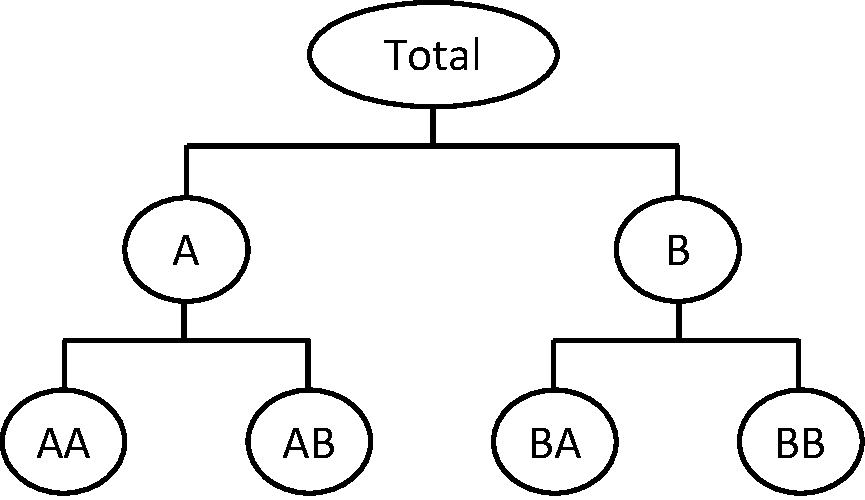
\includegraphics[width=0.4\textwidth,height=\textheight]{figs/hts_example.pdf}

}

\caption{\label{fig-hts}An example of a two-level hierarchical time
series.}

\end{figure}

For example, Figure~\ref{fig-hts} shows a simple hierarchy with
\(n = 7\), \(n_b = 4\), \(n_a = 3\),
\(\bm{y}_t = [y_{\text{Total},t}, y_{\text{A},t}, y_{\text{B},t}, y_{\text{AA},t}, y_{\text{AB},t}, y_{\text{BA},t}, y_{\text{BB},t}]^{\prime}\),
\(\bm{b}_t = [y_{\text{AA},t}, y_{\text{AB},t}, y_{\text{BA},t}, y_{\text{BB},t}]^{\prime}\),
and \[
\bm{S} = \left[
\begin{array}{cccc}
1 & 1 & 1 & 1 \\
1 & 1 & 0 & 0 \\
0 & 0 & 1 & 1 \\
\multicolumn{4}{c}{\bm{I}_4}
\end{array}\right].
\] The notation is general enough to include aggregation constraints
that are non-hierarchical. Please refer to \citet{Hyndman2021-fo} for
further details.

\hypertarget{linear-forecast-reconciliation}{%
\subsection{Linear forecast
reconciliation}\label{linear-forecast-reconciliation}}

Let \(\hat{\bm{y}}_{T+h \mid T} \in \mathbb{R}^n\) be a vector of
\(h\)-step-ahead \emph{base forecasts} for all time series in the
structure, given observations up to and including time \(T\), and
stacked in the same order as \(\bm{y}_t\). We can use any method to
generate these forecasts, but in general they will not be coherent
(i.e., they won't satisfy the constraints). Let
\(\tilde{\bm{y}}_{T+h \mid T} \in \mathbb{R}^n\) denote a vector of
\(h\)-step-ahead \emph{reconciled forecasts} given by
\begin{equation}\protect\hypertarget{eq-lr}{}{
\tilde{\bm{y}}_{T+h \mid T} = \bm{S}\bm{G}_h\hat{\bm{y}}_{T+h \mid T},
}\label{eq-lr}\end{equation} where \(\bm{G}_h\) is an \(n_b \times n\)
weighting matrix and \(\bm{S}\) is an \(n \times n_b\) summing matrix
\citep{Wickramasuriya2019-fc}.

\hypertarget{minimum-trace-reconciliation}{%
\subsubsection*{Minimum trace
reconciliation}\label{minimum-trace-reconciliation}}
\addcontentsline{toc}{subsubsection}{Minimum trace reconciliation}

Let the \(h\)-step-ahead in-sample \emph{base forecast errors} be
defined as
\(\hat{\bm{e}}_{t+h \mid t} = \bm{y}_{t+h} - \hat{\bm{y}}_{t+h \mid t}\),
and the \(h\)-step-ahead \emph{reconciled forecast errors} be given by
\(\tilde{\bm{e}}_{t+h \mid t} = \bm{y}_{t+h} - \tilde{\bm{y}}_{t+h \mid t}\)
for \(t = 1,2,\ldots,T-h\). \citet{Wickramasuriya2019-fc} formulated the
reconciliation problem as minimizing the trace (MinT) of the
\(h\)-step-ahead covariance matrix of the reconciled forecast errors,
\(\operatorname{Var}(\tilde{\bm{e}}_{t+h \mid t})\). Assuming the base
forecasts are unbiased, and that we want the reconciled forecasts to be
unbiased, the unique solution of the minimization problem is given by
\begin{equation}\protect\hypertarget{eq-mint}{}{
\bm{G}_h=\left(\bm{S}^{\prime} \bm{W}_h^{-1} \bm{S}\right)^{-1} \bm{S}^{\prime} \bm{W}_h^{-1},
}\label{eq-mint}\end{equation} where \(\bm{W}_h\) is the positive
definite covariance matrix of the \(h\)-step-ahead base forecast errors.

The trace minimization problem can be reformulated as a least squares
problem with linear constraints:
\begin{equation}\protect\hypertarget{eq-mint_op}{}{
 \min _{\tilde{\bm{y}}_{T+h \mid T}} \quad \frac{1}{2}(\hat{\bm{y}}_{T+h \mid T}-\tilde{\bm{y}}_{T+h \mid T})^{\prime} \bm{W}_{h}^{-1}(\hat{\bm{y}}_{T+h \mid T}-\tilde{\bm{y}}_{T+h \mid T})
 \qquad \text{s.t.} \quad \tilde{\bm{y}}_{T+h \mid T}=\bm{S}\tilde{\bm{b}}_{T+h \mid T},
}\label{eq-mint_op}\end{equation} where
\(\tilde{\bm{b}}_{T+h \mid T} \in \mathbb{R}^{n_b}\) comprises the
\(h\)-step-ahead bottom-level reconciled forecasts, made at time \(T\).
The intuition behind MinT reconciliation is that \textbf{the larger the
estimated variance of the base forecast errors, the larger the range of
adjustments permitted for forecast reconciliation}.

It is challenging to estimate \(\bm{W}_h\), especially for \(h > 1\).
Therefore, it is common to assume \(\bm{W}_h = k_h\bm{W}_1\),
\(\forall h\), where \(k_h > 0\); then the MinT solution of \(\bm{G}\)
does not change with the forecast horizon, \(h\). Hence, we will drop
the subscript \(h\) for ease of exposition. The most popularly used
candidate estimators for \(\bm{W}\) are listed in Table \ref{tbl-bench}.

\begin{table}[!h]
\caption{Forecast reconciliation methods for which different estimators of $\bm{W}$ are used.}\label{tbl-bench}
\centering
\begin{threeparttable}
\begin{tabular}{p{0.7\linewidth}r}
\toprule
Reconciliation method & $\bm{W}_h \propto$\\
\midrule
\textbf{OLS} \citep{Hyndman2011-sd} & $\bm{I}$\\
\textbf{WLSs} \citep{Athanasopoulos2017-jj} & $\operatorname{diag}(\bm{S} \bm{1})$\\
\textbf{WLSv} \citep{Hyndman2016-cz} & $\operatorname{Diag}(\hat{\bm{W}}_1)$\\
\textbf{MinT} \citep{Wickramasuriya2019-fc} & $\hat{\bm{W}}_1$\\
\textbf{MinTs} \citep{Wickramasuriya2019-fc} & $\lambda\operatorname{Diag}(\hat{\bm{W}}_1) + (1-\lambda)\hat{\bm{W}}_1$\\
\bottomrule
\end{tabular}
\begin{tablenotes}[para]
\item Note: $\bm{1}$ is a vector of 1s of size $n_b$, $\operatorname{diag}(\cdot)$ constructs a diagonal matrix using a given vector, $\hat{\bm{W}}_1$ denotes the unbiased covariance estimator based on the in-sample one-step-ahead base forecast errors (i.e., residuals), and $\operatorname{Diag}(\cdot)$ forms a diagonal matrix using the diagonal elements of the input matrix.
\end{tablenotes}
\end{threeparttable}
\end{table}

\hypertarget{relaxation-of-the-unbiasedness-assumptions}{%
\subsubsection*{Relaxation of the unbiasedness
assumptions}\label{relaxation-of-the-unbiasedness-assumptions}}
\addcontentsline{toc}{subsubsection}{Relaxation of the unbiasedness
assumptions}

Both \citet{Hyndman2011-sd} and \citet{Wickramasuriya2019-fc} impose
unbiasedness conditions on the base forecasts and the reconciled
forecasts. \citet{Ben_Taieb2019-be} proposed a reconciliation method
relaxing the assumption of unbiasedness. Specifically, by expanding the
training window incrementally, one observation at a time, they
formulated the reconciliation problem as a regularized empirical risk
minimization (RERM) problem given by \[
\min _{\bm{G}_h} \frac{1}{(T-T_1-h+1)n}\left\|\bm{Y}_{h}^{*}-\hat{\bm{Y}}_{h}^{*} \bm{G}_{h}^{\prime} \bm{S}^{\prime}\right\|_F^2+\lambda\|\operatorname{vec}( \bm{G}_h)\|_1,
\] where \(T_1\) denotes the minimum number of observations used for
model training, \(\left\| \cdot \right\|_F\) is the Frobenius norm,
\(\|\cdot\|_1\) is the \(L_1\) norm, \(\operatorname{vec}(\cdot)\)
denotes the vectorization of a matrix (stacking the columns of the
matrix),
\(\bm{Y}_{h}^{*}=\left[\bm{y}_{T_1+h}, \ldots, \bm{y}_T\right]^{\prime}\),
\(\hat{\bm{Y}}_{h}^{*}=\left[\hat{\bm{y}}_{T_1+h \mid T_1}, \ldots, \hat{\bm{y}}_{T \mid T-h}\right]^{\prime}\),
and \(\lambda \geq 0\) is a regularization parameter.

When \(\lambda = 0\), the problem reduces to an empirical risk
minimization (ERM) problem without regularization. Assuming that the
series in the structure are jointly weakly stationary and
\(\hat{\bm{Y}}_{h}^{*\prime}\hat{\bm{Y}}_{h}^{*}\) is invertible, it has
a closed-form solution given by \[
\hat{\bm{G}}_h = \bm{B}_{h}^{*\prime}\hat{\bm{Y}}_{h}^{*}\left(\hat{\bm{Y}}_{h}^{*\prime}\hat{\bm{Y}}_{h}^{*}\right)^{-1},
\] where
\(\bm{B}_{h}^{*}=\left[\bm{b}_{T_1+h}, \ldots, \bm{b}_T\right]^{\prime}\).
If \(\hat{\bm{Y}}_{h}^{*\prime}\hat{\bm{Y}}_{h}^{*}\) is not invertible,
\citet{Ben_Taieb2019-be} suggested using a generalized inverse. When
\(\lambda > 0\), imposing the \(L_1\) penalty on \(\bm{G}_h\) will
introduce sparsity and reduce estimation variance, albeit at the cost of
introducing some bias.

\citet{Wickramasuriya2021-am} proposed an empirical MinT
(\textbf{EMinT}) solution without the unbiasedness constraint by
minimizing the trace of the covariance matrix of the reconciled forecast
errors, \(\operatorname{Var}(\tilde{\bm{e}}_{T+h \mid T})\). Assuming
the series are jointly weakly stationary, she derived the solution \[
\hat{\bm{G}}_{h} = \bm{B}_{h}^{\prime}\hat{\bm{Y}}_{h}\left(\hat{\bm{Y}}_{h}^{\prime}\hat{\bm{Y}}_{h}\right)^{-1},
\] where
\(\bm{B}_{h}=\left[\bm{b}_{h}, \ldots, \bm{b}_T\right]^{\prime}\), and
\(\hat{\bm{Y}}_{h}=\left[\hat{\bm{y}}_{h \mid 0}, \ldots, \hat{\bm{y}}_{T \mid T-h}\right]^{\prime}\).

The difference between EMinT and ERM lies in the data sources, as EMinT
uses in-sample observations and base forecasts, while ERM relies on
observations and base forecasts from a holdout validation set. Both ERM
and EMinT consider an estimate of \(\bm{G}\) that changes over the
forecast horizon, which is why we keep the subscript \(h\) here.

A challenge in forecast reconciliation arises when some base forecasts
perform poorly, as the role of the weighting matrix \(\bm{G}\) is to
assimilate \emph{all} base forecasts and map them into bottom-level
disaggregated forecasts, which are subsequently summed by \(\bm{S}\).
While the RERM method proposed by \citet{Ben_Taieb2019-be} introduces
sparsity by shrinking some elements of \(\bm{G}\) towards zero, it
remains incapable of mitigating the adverse impact of underperforming
base forecasts. Moreover, the method is time-consuming because it uses
expanding windows to recursively generate out-of-sample base forecasts.

We therefore propose two new forecast reconciliation methods involving
time series selection: constrained out-of-sample (under the unbiasedness
assumption) and unconstrained in-sample (without the unbiasedness
assumption). These methods aim to address the negative effect of some
poor base forecasts on the overall performance of the reconciled
forecasts. Additionally, through the incorporation of regularization in
the objective function, our method improves reconciliation outcomes
produced with a ``poor'' choice of \(\bm{W}\).

\hypertarget{sec-methodology}{%
\section{Forecast reconciliation with time series
selection}\label{sec-methodology}}

In this section, we introduce our methods for keeping forecasts of an
automatically selected set of series, identified as harmful to
reconciliation, unused in forming reconciled forecasts, i.e., forecast
reconciliation with time series selection. Section~\ref{sec-constrained}
introduces constrained reconciliation methods with selection that
formulate the problem based on out-of-sample base forecasts, while
Section~\ref{sec-unconstrained} presents an unconstrained reconciliation
method with selection, where we formulate the problem based on in-sample
observations and base forecasts.

\hypertarget{sec-constrained}{%
\subsection{Series selection with unbiasedness
constraint}\label{sec-constrained}}

As \(\bm{S}\) is fixed and \(\hat{\bm{y}}_{T+h \mid T}\) is given, once
we get the estimation of \(\bm{G}\), the linear reconciliation
performance is determined, as shown in Equation~\ref{eq-lr}. In this
section, the subscript \(h\) is dropped as we assume \(\bm{W}\) and
\(\bm{G}\) do not vary with the forecast horizon. A natural way to keep
forecasts of some series unused in reconciliation is through controlling
the number of nonzero column entries in \(\bm{G}\). This leads to a
generalization of the MinT optimization problem by applying an
additional penalty to the objective function. More precisely, let
\(\hat{\bm{y}}:=\hat{\bm{y}}_{T+1 \mid T}\), we consider the
optimization problem given by
\begin{equation}\protect\hypertarget{eq-op_u}{}{
\min _{\bm{G}} \quad \frac{1}{2}\left(\hat{\bm{y}}-\bm{SG}\hat{\bm{y}}\right)^{\prime} \bm{W}^{-1}\left(\hat{\bm{y}}-\bm{SG}\hat{\bm{y}}\right)
+ \lambda\mathfrak{g}(\bm{G}) \qquad \text{s.t.} \quad \bm{GS}=\bm{I},
}\label{eq-op_u}\end{equation} where \(\mathfrak{g}(\cdot)\) is defined
as an exterior penalty function designed to penalize the columns of
\(\bm{G}\) towards zero, with \(\lambda\) is the corresponding penalty
coefficient. Thus, this can be considered as \emph{a grouped variable
selection problem}, with each group corresponding to a column of
\(\bm{G}\). Obviously, these groups are not overlapped. The constraint,
\(\bm{GS}=\bm{I}\), reflects the assumption that base forecasts and
reconciled forecasts are unbiased. When \(\lambda = 0\), \(\forall h\),
the problem reduces to the MinT optimization problem in
Equation~\ref{eq-mint_op} with a closed-form solution given by
Equation~\ref{eq-mint}.

\textbf{Proposition 1.} \emph{Under the assumption of unbiasedness, the
count of nonzero column entries of} \(\bm{G}\) (\emph{i.e., the number
of time series selected for reconciliation}), \emph{derived through
solving Equation~\ref{eq-op_u}, is at least equal to the number of time
series at the bottom level. In addition, we can restore the full
hierarchical structure by aggregating/disaggregating the selected time
series.}

\emph{Proof}. According to the unbiasedness constraint
\(\bm{GS}=\bm{I}\), we have \[
\min \left(\operatorname{rank}(\bm{G}), \operatorname{rank}(\bm{S})\right) \geq \operatorname{rank}(\bm{I}_{n_b})=n_b,
\] which indicates that the count of nonzero column entries of
\(\bm{G}\) is at least equal to \(n_b\).

Let \(\bm{X}_{\cdot \mathbb{S}} \in \mathbb{R}^{r \times |\mathbb{S}|}\)
denote the submatrix of the \(r \times c\) matrix \(\bm{X}\) with column
indices forming a set \(\mathbb{S}\) (and when \(\mathbb{S} = \{j\}\),
we simply use \(\bm{X}_{\cdot j}\)), where \(|\mathbb{S}|\) denotes the
size of the set \(\mathbb{S}\). Similarly, let
\(\bm{X}_{\mathbb{S}\cdot} \in \mathbb{R}^{|\mathbb{S}| \times c}\)
denote the submatrix of \(\bm{X}\) whose rows are indexed by a set
\(\mathbb{S}\) (and when \(\mathbb{S} = \{i\}\), we simply use
\(\bm{X}_{i\cdot}\)). Assuming that the set \(\mathbb{S}\) consists of
the indices of nonzero columns in the solution of
Equation~\ref{eq-op_u}, \(\hat{\bm{G}}\), the following equations hold:
\[
\bm{G}\bm{S} = \hat{\bm{G}}_{\cdot \mathbb{S}}\bm{S}_{\mathbb{S}\cdot} = \bm{I},
\qquad\text{and}\qquad
\min \left(\operatorname{rank}(\hat{\bm{G}}_{\cdot \mathbb{S}}), \operatorname{rank}(\bm{S}_{\mathbb{S}\cdot})\right) \geq \operatorname{rank}(\bm{I}_{n_b})=n_b.
\] Additionally, we have
\(\operatorname{rank}(\bm{S}_{\mathbb{S}\cdot}) \leq n_b\) as \(\bm{S}\)
has \(n_b\) columns. Therefore, we can conclude that
\(\operatorname{rank}(\bm{S}_{\mathbb{S}\cdot}) = n_b\). Moreover, we
have \[
\bm{y}_t = \bm{S}\bm{b}_t = \bm{S}\bm{G}\bm{S}\bm{b}_t=\bm{S}\hat{\bm{G}}_{\cdot\mathbb{S}}\bm{S}_{\mathbb{S}\cdot}\bm{b}_t=\bm{S}\hat{\bm{G}}_{\cdot \mathbb{S}}(\bm{y}_t)_{\mathbb{S}},
\] which implies that the hierarchical structure can be fully restored
by aggregating/disaggregating the selected time series denoted by
\((\bm{y}_{t})_{\mathbb{S}}\).

For example, consider the simple hierarchy shown in
Figure~\ref{fig-hts}, it is not possible for our constrained
reconciliation methods with selection to simultaneously zero out columns
of \(\bm{G}\) associated with series AA and AB. However, it is possible
to zero out columns related to series AA and BA simultaneously.

\textbf{Proposition 2.} \emph{The optimization problem in
Equation~\ref{eq-op_u} can be reformulated as a least squares problem
with regularization and linear equality constraint as follows:}
\begin{equation}\protect\hypertarget{eq-op_u_reg}{}{
\begin{aligned}
& \min _{\operatorname{vec}(\bm{G})} \quad \frac{1}{2}\left(\hat{\bm{y}}-\left(\hat{\bm{y}}^{\prime} \otimes \bm{S}\right) \operatorname{vec}(\bm{G})\right)^{\prime} \bm{W}^{-1}\left(\hat{\bm{y}}-\left(\hat{\bm{y}}^{\prime} \otimes \bm{S}\right) \operatorname{vec}(\bm{G})\right) + \lambda\mathfrak{g}\left(\operatorname{vec}(\bm{G})\right) \\
& \text{s.t.} \quad \left(\bm{S}^{\prime} \otimes \bm{I}_{n_b}\right) \operatorname{vec}(\bm{G})=\operatorname{vec}(\bm{I}_{n_b}),
\end{aligned}
}\label{eq-op_u_reg}\end{equation} \emph{which is characterized as a
high-dimensional problem in which the number of features, denoted as}
\(p = n_b \times n\)\emph{, is much larger than the number of
observations,} \(n\)\emph{.}

\emph{Proof.} We have \[
\begin{aligned}
& \operatorname{vec}\left(\hat{\bm{y}}\right) = \hat{\bm{y}}, \\
& \operatorname{vec}\left(\bm{SG}\hat{\bm{y}}\right) = \left(\hat{\bm{y}}^{\prime} \otimes \bm{S}\right) \operatorname{vec}(\bm{G}), \\
& \operatorname{vec}\left(\bm{GS}\right) = \operatorname{vec}\left(\bm{I}_{n_b}\bm{GS}\right) = \left(\bm{S}^{\prime} \otimes \bm{I}_{n_b}\right) \operatorname{vec}(\bm{G}).
\end{aligned}
\] Substituting the terms in Equation~\ref{eq-op_u} with these
expressions, the previous problem now takes the form of a regression
problem with an additional regularization term and an equality
constraint on the coefficients, as shown in Equation~\ref{eq-op_u_reg}.

Moving forward, we present three classes of regularizations we use to
establish forecast reconciliation with series selection, resulting in
the consideration of three optimization problems: (i) group best-subset
selection with ridge regularization, (ii) intuitive method with \(L_0\)
regularization, and (iii) group lasso method.

\hypertarget{sec-subset}{%
\subsubsection{Group best-subset selection with ridge
regularization}\label{sec-subset}}

In high-dimensional regime with \(p \gg n\), a common desiderata is to
assume that the true regression coefficient (i.e.,
\(\operatorname{vec}(\bm{G})\) in our problem) is sparse. We propose to
apply a combination of \(L_0\) and \(L_2\) regularization as the
exterior penalty function to control the nonzero column entries in
\(\bm{G}\): \begin{align}
\min _{\operatorname{vec}(\bm{G})} \quad & \frac{1}{2}\left(\hat{\bm{y}}-\left(\hat{\bm{y}}^{\prime} \otimes \bm{S}\right) \operatorname{vec}(\bm{G})\right)^{\prime} \bm{W}^{-1}\left(\hat{\bm{y}}-\left(\hat{\bm{y}}^{\prime} \otimes \bm{S}\right) \operatorname{vec}(\bm{G})\right) + \lambda_0 \sum_{j=1}^n 1\left(\bm{G}_{\cdot j} \neq \bm{0}\right) + \lambda_2 \left\|\operatorname{vec}\left(\bm{G}\right)\right\|_2^2 \nonumber\\
\text{s.t.} \quad & \left(\bm{S}^{\prime} \otimes \bm{I}_{n_b}\right) \operatorname{vec}(\bm{G})=\operatorname{vec}(\bm{I}_{n_b}), \label{eq-subset}
\end{align} where \(1(\cdot)\) is the indicator function,
\(\lambda_0 \geq 0\) controls the number of nonzero columns of
\(\bm{G}\) selected, \(\lambda_2 \geq 0\) controls the strength of the
ridge regularization, and \(\|\cdot\|_2\) is the \(L_2\) norm. In a
hierarchical or grouped time series context, the parameter of interest
in Equation \ref{eq-subset}, \(\operatorname{vec}(\bm{G})\), has an
inherent non-overlapping grouping structure, wherein each group
corresponds to a single column of \(\bm{G}\), each with a size of
\(n_b\). Therefore, we refer to this reconciliation method as
\emph{group best-subset selection with ridge regularization}. In the
results that follow, we label the \textbf{Subset} method differently
based on various estimators for \(\bm{W}\), referring to them as
\textbf{OLS-subset}, \textbf{WLSs-subset}, \textbf{WLSv-subset},
\textbf{MinT-subset}, and \textbf{MinTs-subset}, respectively.

The inclusion of the ridge term in Equation \ref{eq-subset} is motivated
by earlier work on best-subset selection
\citep[e.g.,][]{Hazimeh2020-xd, Mazumder2022-hx}, which suggests that
additional ridge regularization can mitigate the poor predictive
performance of best-subset selection method in the low signal-to-noise
ratio (SNR) regimes.

We present a Big-M based mixed integer programming (MIP) formulation for
problem in Equation \ref{eq-subset} given by
\begin{align} \label{eq-subset_mip}
\min _{\operatorname{vec}(\bm{G}), \bm{z}, \check{\bm{e}}, \bm{g}^{+}} & \frac{1}{2}\check{\bm{e}}^{\prime} \bm{W}^{-1}\check{\bm{e}} + \lambda_0 \sum_{j=1}^n z_j + \lambda_2 \bm{g}^{+\prime}\bm{g}^{+} \\
\text{s.t.} \quad & \left(\bm{S}^{\prime} \otimes \bm{I}_{n_b}\right) \operatorname{vec}(\bm{G})=\operatorname{vec}\left(\bm{I}_{n_b}\right)\nonumber \\
& \hat{\bm{y}}-\left(\hat{\bm{y}}^{\prime} \otimes \bm{S}\right)\operatorname{vec}(\bm{G}) = \check{\bm{e}} \nonumber\\
& \sum_{i=1}^{n_b} g_{i + (j-1) n_b}^{+} \leqslant \mathcal{M} z_j, \quad j \in[n] \nonumber\\
& \bm{g}^{+} \geqslant \operatorname{vec}(\bm{G}) \nonumber\\
& \bm{g}^{+} \geqslant-\operatorname{vec}(\bm{G}) \nonumber\\
& z_j \in\{0,1\}, \quad j \in[n],
\end{align} where \(\mathcal{M}\) is a Big-M parameter (a-priori
specified) that is sufficiently large such that some optimal solution,
say \(\bm{g}^{+*}\), to Equation \ref{eq-subset_mip} satisfies
\(\max _{j \in [n]}\sum_{i=1}^{n_b} g_{i + (j-1) n_b}^{+} \leqslant \mathcal{M}\),
the binary variable \(z_j\) controls whether all the regression
coefficients, \(\operatorname{vec}(\bm{G})\), in group \(j\) are zero or
not, i.e., \(z_j=0\) implies that \(\bm{G}_{\cdot j}=\bm{0}\), and
\(z_j=1\) implies that
\(\sum_{i=1}^{n_b} g_{i + (j-1) n_b}^{+} \leqslant \mathcal{M}\). Such
Big-M formulations are commonly used in MIP problems to model relations
between discrete and continuous variables, and have been recently
explored in regression with \(L_0\) regularization
\citep{Bertsimas2016-ig}. The problem is a mixed integer quadratic
program (MIQP) that can be solved using commercial MIP solvers, e.g.,
Gurobi and CPLEX.

\textbf{Parameter tuning.} To avoid computationally-expensive
cross-validation, we tune the parameters to minimize the sum of squared
reconciled forecast errors on the truncated training set, comprising
only the \(\max\{h, s\}\) observations closest to the forecast origin,
where \(s\) is the seasonal period for seasonal data and \(s=T\) for
non-seasonal data. Let
\(\lambda_{0}^{1} = \frac{1}{2}\left(\hat{\bm{y}}-\tilde{\bm{y}}^{\text{bench}}\right)^{\prime} \bm{W}^{-1}\left(\hat{\bm{y}}-\tilde{\bm{y}}^{\text{bench}}\right)\)
that captures the scale of first term in the objective function, where
\(\tilde{\bm{y}}^{\text{bench}}\) is a vector of reconciled forecasts
obtained using Equation~\ref{eq-mint} with same estimator of \(\bm{W}\),
and define \(\lambda_{0}^{k} = 0.0001\lambda_{0}^{1}\). For the
parameter \(\lambda_0\), we consider a grid of \(k+1\) values,
\(\{\lambda_{0}^{1},\dots,\lambda_{0}^{k}, 0\}\), where
\(\lambda_{0}^{j} = \lambda_{0}^{1}\left(\lambda_{0}^{k} / \lambda_{0}^{1}\right)^{(j-1) / (k-1)}\)
for \(j \in [k]\). So \(\lambda_{0}^{1},\dots,\lambda_{0}^{k}\) is a
sequence decreasing on the log scale. We use a grid of six values for
the parameter \(\lambda_2\),
\(\{0, 10^{-2}, 10^{-1}, 10^{0}, 10^{1}, 10^{2}\}\). Therefore, we tune
over a two-dimensional grid of \((k+1) \times 6\) values to find the
optimal combination of \(\lambda_0\) and \(\lambda_2\).

\textbf{Computation details.} The MIQP problem in Equation
\ref{eq-subset_mip} is NP-Hard and computationally intensive.
\citet{Bertsimas2016-ig} showed that commercial MIP solvers are capable
of tackling problem instances for \(p\) up to a thousand. To address
larger instances, there has been impressive work on developing MIP-based
approches for solving \(L_0\)-regularized regression problem, e.g.,
\citet{Bertsimas2016-ig}, \citet{Hazimeh2020-xd}, and
\citet{Hazimeh2022-hc}. However, it is challenging to extend their
approaches to accommodate additional constraints within the optimization
problem. Despite the potential sluggishness of handling large instances
with commercial MIP solvers, in our experiments, we use Gurobi to solve
our problem in Equation \ref{eq-subset_mip} by configuring parameters
such as MIPGap = \(0.001\) and TimeLimit = \(600\) seconds for cases
with \(p > 1000\). This enables us to terminate the solver before
reaching the global optimum and return a suboptimal solution instead.
This strategy is motivated by our need to consider numerous parameter
candidates, and the final solution will be validated against the
training set, which prevents the utilization of a very poor estimate of
\(\bm{G}\).

\hypertarget{sec-intuitive}{%
\subsubsection{\texorpdfstring{Intuitive method with \(L_0\)
regularization}{Intuitive method with L\_0 regularization}}\label{sec-intuitive}}

Instead of estimating the entire matrix \(\bm{G}\) in
Section~\ref{sec-subset}, we leverage the MinT solution in
Equation~\ref{eq-mint} to streamline the optimization problem under
consideration. Specifically, we define \(\bar{\bm{S}} = \bm{A}\bm{S}\),
where \(\bm{A} = \operatorname{diag}(\bm{z})\) is an \(n \times n\)
diagonal matrix, and \(\bm{z}\) is an \(n\)-dimensional vector with
elements either equal to 0 or 1. Taking the MinT solution in
Equation~\ref{eq-mint}, we have
\(\bar{\bm{G}} = (\bm{S}^{\prime}\bm{A}^{\prime}\bm{W}^{-1}\bm{A}\bm{S})^{-1}\bm{S}^{\prime}\bm{A}^{\prime}\bm{W}^{-1}\).
Given fixed \(\bm{S}\) and estimation of \(\bm{W}\), \(\bar{\bm{G}}\) is
entirely determined by \(\bm{A}\). By this way, when the \(j\)th
diagonal element of \(\bm{A}\) equals zero, the \(j\)th column of
\(\bar{\bm{G}}\) becomes entirely composed of zeros. Therefore, the
optimization problem can be reduced to an integer quadratic programming
(IQP) problem in which all of the variables are restricted to be
integers: \begin{align*}
\min _{\bm{A}} \quad & \frac{1}{2}\left(\hat{\bm{y}}-\bm{S}\bar{\bm{G}}\hat{\bm{y}}\right)^{\prime} \bm{W}^{-1}\left(\hat{\bm{y}}-\bm{S}\bar{\bm{G}}\hat{\bm{y}}\right) + \lambda_0 \sum_{j=1}^n \bm{A}_{jj} \\
\text{s.t.} \quad & \bar{\bm{G}} = (\bm{S}^{\prime}\bm{A}^{\prime}\bm{W}^{-1}\bm{A}\bm{S})^{-1}\bm{S}^{\prime}\bm{A}^{\prime}\bm{W}^{-1} \qquad\text{and}\qquad \bar{\bm{G}}\bm{S} = \bm{I},
\end{align*} where \(\lambda_0 \geq 0\) controls the number of nonzero
diagonal elements in \(\bm{A}\), consequently affecting the number of
nonzero columns (i.e., selected time series) in \(\bm{G}\). We refer to
this reconciliation method as \emph{intuitive method with} \(L_0\)
\emph{regularization}. In the results that follow, we label the
\textbf{Intuitive} method differently based on various estimators for
\(\bm{W}\), referring to them as \textbf{OLS-intuitive},
\textbf{WLSs-intuitive}, \textbf{WLSv-intuitive},
\textbf{MinT-intuitive}, and \textbf{MinTs-intuitive}, respectively.

We should note that implementing grouped variable selection with this
optimization problem can be challenging because it imposes restrictions
on the parameter of interest (\(\bar{\bm{G}}\)) to ensure it adheres
rigorously to the analytical solution of MinT while making the
selection. Therefore, the resulting solution tends to be dense and may
not have zero columns.

To ensure the invertibility of
\(\bm{S}^{\prime}\bm{A}^{\prime}\bm{W}^{-1}\bm{A}\bm{S}\) and make the
problem compatible with Gurobi, we reformulate the problem as
\begin{equation}\protect\hypertarget{eq-intuitive_mip}{}{
\begin{aligned}
\min _{\bm{A},\bar{\bm{G}},\bm{C},\check{\bm{e}},\bm{z}} \quad & \frac{1}{2}\check{\bm{e}}^{\prime} \bm{W}^{-1}\check{\bm{e}} + \lambda_0 \sum_{j=1}^n z_j \\
\text{s.t.} \quad & \bar{\bm{G}}\bm{S} = \bm{I} \\
& \hat{\bm{y}}-\left(\hat{\bm{y}}^{\prime} \otimes \bm{S}\right)\operatorname{vec}(\bar{\bm{G}}) = \check{\bm{e}} \\
& \bar{\bm{G}}\bm{A}\bm{S} = \bm{I} \\
& \bar{\bm{G}} = \bm{C}\bm{S}^{\prime}\bm{A}^{\prime}\bm{W}^{-1} \\
& z_j \in\{0,1\}, \quad j \in[n].
\end{aligned}
}\label{eq-intuitive_mip}\end{equation}

\textbf{Parameter tuning.} Similarly to the setup in
Section~\ref{sec-subset}, we select the tuning parameter, \(\lambda_0\),
by minimizing the sum of squared reconciled forecast errors on a
truncated training set, comprising only the \(\max\{h, s\}\)
observations occurred prior to the forecast origin. Let
\(\lambda_{0}^{1} = \frac{1}{2}\left(\hat{\bm{y}}-\tilde{\bm{y}}^{\text{bench}}\right)^{\prime} \bm{W}^{-1}\left(\hat{\bm{y}}-\tilde{\bm{y}}^{\text{bench}}\right)\),
and \(\lambda_{0}^{k} = 0.0001\lambda_{0}^{1}\), the collection of
candidate values for \(\lambda_0\) we consider is
\(\{\lambda_{0}^{1},\dots,\lambda_{0}^{k}, 0\}\), where
\(\lambda_{0}^{j} = \lambda_{0}^{1}\left(\lambda_{0}^{k} / \lambda_{0}^{1}\right)^{(j-1) / (k-1)}\)
for \(j \in [k]\).

\textbf{Computation details.} Following a setup akin to that in
Section~\ref{sec-subset}, we employ Gurobi to solve
Equation~\ref{eq-intuitive_mip} by configuring parameters such as MIPGap
= \(0.001\) and TimeLimit = \(600\) seconds for problems with
\(p > 1000\).

\hypertarget{sec-lasso}{%
\subsubsection{Group lasso method}\label{sec-lasso}}

Lasso is another popular method for selection and estimation of
parameters in the context of linear regression. \citet{Yuan2006-mw}
introduced the group lasso method that can be used when there is a
grouped structure among the variables. Here, we consider \emph{a group
lasso problem under the unbiasedness assumption} given by
\begin{equation}\protect\hypertarget{eq-lasso}{}{
\begin{aligned}
\min _{\bm{G}} \quad & \frac{1}{2}\left(\hat{\bm{y}}-\left(\hat{\bm{y}}^{\prime} \otimes \bm{S}\right) \operatorname{vec}(\bm{G})\right)^{\prime} \bm{W}^{-1}\left(\hat{\bm{y}}-\left(\hat{\bm{y}}^{\prime} \otimes \bm{S}\right) \operatorname{vec}(\bm{G})\right) + \lambda \sum_{j=1}^n w_j \left\|\bm{G}_{\cdot j}\right\|_2 \\
\text{s.t.} \quad & \left(\bm{S}^{\prime} \otimes \bm{I}_{n_b}\right) \operatorname{vec}(\bm{G})=\operatorname{vec}\left(\bm{I}_{n_b}\right),
\end{aligned}
}\label{eq-lasso}\end{equation} where \(\lambda \geq 0\) is a tuning
parameter, \(w_j \neq 0\) is the penalty weight assigned in
\(\bm{G}_{\cdot j}\) to make model more flexible, and the second term in
the objective is the penalty function that is intermediate between the
\(L_1\)-penalty that is used in the lasso and the \(L_2\)-penalty that
is used in ridge regression. In the results that follow, we label the
\textbf{Lasso} method based on various estimators for \(\bm{W}\),
referring to them as \textbf{OLS-lasso}, \textbf{WLSs-lasso},
\textbf{WLSv-lasso}, \textbf{MinT-lasso}, and \textbf{MinTs-lasso},
respectively.

Next, we present the second order cone programming (SOCP) formulation
for the group lasso based estimators given by
\begin{equation}\protect\hypertarget{eq-lasso_socp}{}{
\begin{aligned}
\min _{\operatorname{vec}(\bm{G}), \check{\bm{e}}, \bm{g}^{+}} & \frac{1}{2}\check{\bm{e}}^{\prime} \bm{W}_h^{-1}\check{\bm{e}} + \lambda \sum_{j=1}^n w_j c_j \\
\text{s.t.} \quad & \left(\bm{S}^{\prime} \otimes \bm{I}_{n_b}\right) \operatorname{vec}(\bm{G})=\operatorname{vec}\left(\bm{I}_{n_b}\right) \\
& \hat{\bm{y}}-\left(\hat{\bm{y}}^{\prime} \otimes \bm{S}\right) \operatorname{vec}(\bm{G}) = \check{\bm{e}} \\
& c_j = \sqrt{\sum_{i=1}^{n_b} g_{i + (j-1) n_b}^{+2}}, \quad j \in[n].
\end{aligned}
}\label{eq-lasso_socp}\end{equation} Equation~\ref{eq-lasso_socp}
includes additional auxiliary variables \(c_j \in \mathbb{R}_{\geq 0}\),
\(j \in [n]\), and second order cone constraints,
\(c_j = \sqrt{\sum_{i=1}^{n_b} g_{i + (j-1) n_b}^{+2}}\) for
\(j \in[n]\).

Compared to the previous two methods we proposed, the group lasso method
is computationally friendlier. Nonetheless, \citet{Hazimeh2023-ie}
demonstrated, both empirically and theoretically, that group
\(L_0\)-regularized method exhibits advantages over its group lasso
counterpart across a range of regimes. Group lasso can either be highly
dense or possess non-zero coefficients that are overly shrunk. This
issue becomes more pronounced when the groups are correlated with each
other as group lasso tends to retain all correlated groups instead of
seeking a more concise model.

\textbf{Penalty weights and parameter tuning.} In the context of group
lasso, the default choice for the penalty weight, \(w_j\), is
\(\sqrt{p_j}\), where \(p_j\) is the size of each group (in our case,
\(p_j = n_b\)). In our experiments, we allocate different penalty
weights to each group using
\(w_j = 1/\left\|\bm{G}_{\cdot j}^{\text{bench}}\right\|_2\), which
allows us to account for variations in scale across different time
series in the structure.

We compute the group lasso over \(k+1\) values of the tuning parameter
\(\lambda\), and select the tuning parameter by optimizing the sum of
squared reconciled forecast errors on a truncated training set,
consisting only of \(\max\{h, s\}\) observations occurred prior to the
forecast origin. The collection of candidate values for \(\lambda\)
under consideration is \(\{\lambda^{1},\dots,\lambda^{k}, 0\}\), where
\(\lambda^{1} = \max _{j=1, \ldots, n}\left\|-\left(\left(\hat{\bm{y}}^{\prime} \otimes \bm{S}\right)_{\cdot j^{*}}\right)^{\prime} \bm{W}^{-1} \hat{\bm{y}}\right\|_2 / w_j\),
\(\lambda^{k} = 0.0001\lambda^{1}\), and
\(\lambda^{j} = \lambda^{1}\left(\lambda^{k} / \lambda^{1}\right)^{(j-1) / (k-1)}\)
for \(j \in [k]\).

\textbf{Proposition 3.} \emph{Ignoring the unbiasedness constraint, we
define} \(\lambda^{1}\) \emph{as the smallest} \(\lambda\) \emph{value
such that all predictors in the group lasso problem have zero
coefficients. Then we have} \[
\lambda^{1} = \max _{j=1, \ldots, n}\left\|-\left(\left(\hat{\bm{y}}^{\prime} \otimes \bm{S}\right)_{\cdot j^{*}}\right)^{\prime} \bm{W}^{-1} \hat{\bm{y}}\right\|_2 / w_j,
\] \emph{where} \(j^{*}\) \emph{denotes the column index of}
\(\hat{\bm{y}}^{\prime} \otimes \bm{S}\) \emph{that corresponds to the}
\(j\)\emph{th column of} \(\bm{G}\)\emph{.}

\emph{Proof.} Denote \(\bm{\beta} = \operatorname{vec}(\bm{G})\), and
the first term in the objective of Equation~\ref{eq-lasso} as
\(L\left(\bm{\beta} \mid \bm{D}\right)\), where \(\bm{D}\) is the
working data
\(\{\hat{\bm{y}} , \hat{\bm{y}}^{\prime} \otimes \bm{S}\}\). Ignoring
the unbiasedness constraint, we define \(\lambda^{1}\) as the smallest
\(\lambda\) value such that all predictors in the group lasso problem
have zero coefficients, i.e., the solution at \(\lambda^{1}\) is
\(\hat{\bm{\beta}}^{1}=\bm{0}\). (Note that there is no intercept in our
problem.) Under the Karush-Kuhn-Tucker conditions, we have \[
\lambda^{1}
 = \max _{j=1, \ldots, n}\left\|\left[\nabla L\left(\hat{\bm{\beta}}^{1} \mid \bm{D}\right)\right]^{(j)}\right\|_2 / w_j
 = \max _{j=1, \ldots, n}\left\|-\left(\left(\hat{\bm{y}}^{\prime} \otimes \bm{S}\right)_{\cdot j^{*}}\right)^{\prime} \bm{W}^{-1} \hat{\bm{y}}\right\|_2 / w_j.
\]

\textbf{Computation details.} Due to the incorporation of the
unbiasedness constraint, we can not directly use some open-source
packages designed for group lasso. Consequently, we employ Gurobi to
solve the SOCP problem, configuring it by setting OptimalityTol =
\(0.0001\).

\hypertarget{sec-unconstrained}{%
\subsection{Series selection method without unbiasedness
constraint}\label{sec-unconstrained}}

In this section, we relax the unbiasedness constraint,
\(\bm{GS} = \bm{I}\), and introduce a reconciliation method with
selection that relies on in-sample observations and fitted values. Let
\(\bm{Y} \in \mathbb{R}^{T \times n}\) denote a matrix comprising
observations from all time series on the training set in the structure,
and \(\hat{\bm{Y}} \in \mathbb{R}^{T \times n}\) denote a matrix of
in-sample one-step-ahead forecasts (i.e., fitted values) for all time
series. The proposed \emph{empirical group lasso} method considers the
optimization problem \[
\min _{\bm{G}} \quad \frac{1}{2 T} \left\|\bm{Y}-\hat{\bm{Y}} \bm{G}^{\prime} \bm{S}^{\prime}\right\|_F^2 + \lambda \sum_{j=1}^n w_j \left\|\bm{G}_{\cdot j}\right\|_2,
\] where \(\lambda \geq 0\) is a tuning parameter, \(w_j \neq 0\) is the
penalty weight assigned in \(\bm{G}_{\cdot j}\) to make a more flexible
model. We rewrite the problem as \[
\min _{\operatorname{vec}(\bm{G})} \quad \frac{1}{2 T} \left\|\operatorname{vec}(\bm{Y})-(\bm{S} \otimes \hat{\bm{Y}}) \operatorname{vec}\left(\bm{G}^{\prime}\right)\right\|_2^2 + \lambda \sum_{j=1}^n w_j \left\|\bm{G}_{\cdot j}\right\|_2,
\] which becomes a standard group lasso problem, with
\(\operatorname{vec}(\bm{Y})\) serving as the dependent variable and
\(\bm{S} \otimes \hat{\bm{Y}}\) as the covariate matrix. We denote this
as \textbf{Elasso} in the results that follow.

Upon relaxing the unbiasedness constraint, the number of non-zero column
entries in the solution for \(\bm{G}\) may be less than the number of
time series at the bottom level. This differs from the series selection
methods with an unbiasedness constraint that we introduced in
Section~\ref{sec-constrained}. In an extreme scenario, it can happen
that the solution takes the form of a top-down
\(\bm{G}_{TD}=[\bm{p} \mid \bm{O}_{n_b \times (n-1)}]\), where only the
column corresponding to the top level (most aggregated level) retains
non-zero values, and \(\bm{p} = (p_1, p_2, \ldots, p_{n_b})\) is a
proportionality vector obtained based on in-sample reconciled forecast
errors.

We also explored the empirical version of group best-subset selection
with ridge regularization and intuitive method with \(L_0\)
regularization in which we do not impose the unbiasedness constraint. It
is worth mentioning that \citet{Hazimeh2023-ie} presented a new
algorithmic framework for formulating the group \(L_0\) problem with
ridge regularization and provided the \textbf{L0Group} Python package
for implementation. However, our experiments showed that this algorithm
can not terminate within five hours for typical instances with
\(p \sim 10^4\). Therefore, in this paper, we only present the empirical
group lasso method for series selection without unbiasedness constraint.

\textbf{Penalty weights and parameter tuning.} Similarly to the setup in
Section~\ref{sec-lasso}, we assign different penalty weights to each
group by setting
\(w_j = 1/\left\|\bm{G}_{\cdot j}^{\text{OLS}}\right\|_2\), where
\(\bm{G}^{\text{OLS}}\) is the solution obtained by the OLS estimator of
\(\bm{W}\). Given a fixed tuning parameter value, we solve the target
optimization problem by considering the initial \(T-T_v\) observations,
where \(T_v = \max\{h, s\}\) for seasonal time series and
\(T_v = \lfloor \frac{1}{10}T \rfloor\) for non-seasonal time series.
Then we select the tuning parameter, \(\lambda\), by minimizing the sum
of squared reconciled forecast errors on a truncated training set,
comprising only the \(T_v\) observations closest to the forecast origin.
Specifically, we form the set of candidate values for \(\lambda\) as
\(\{\lambda^{1},\dots,\lambda^{k}, 0\}\), where
\(\lambda^{1} = \max _{j=1, \ldots, n}\left\|-\frac{1}{N}\left(\left(\bm{S} \otimes \hat{\bm{Y}}\right)_{\cdot j*}\right)^{\prime} \operatorname{vec}(\bm{Y})\right\|_2 / w_j\),
\(\lambda^{k} = 0.0001\lambda^{1}\), and
\(\lambda^{j} = \lambda^{1}\left(\lambda^{k} / \lambda^{1}\right)^{(j-1) / (k-1)}\)
for \(j \in [k]\). Following the same derivation as in the proof of
\textbf{Proposition 3}, \(\lambda^{1}\) is the smallest \(\lambda\)
value such that all predictors in the empirical group lasso problem have
zero coefficients, i.e., \(\bm{G} = \bm{O}\). Note that we need to
resolve the optimization problem based the whole training set by using
the optimal tuning parameter to obtain the final solution.

\textbf{Computation details.} While there are open-source packages
available for solving a group lasso problem, they are still relatively
slow when applied to large instance for practical usage. For example,
given a specific value for the parameter, \(\lambda\), our experiments
observed that, using the \textbf{gglasso} R package, we can not obtain a
solution within five hours for typical instances with \(p \sim 10^4\).
Instead, we use Gurobi to solve the problem based on the SOCP
formulation for the empirical group lasso which aligns with
Equation~\ref{eq-lasso_socp} but omits the unbiasedness constraint.

\hypertarget{sec-simulations}{%
\section{Monte Carlo simulations}\label{sec-simulations}}

To evaluate the performance of various reconciliation methods with time
series selection outlined in Section~\ref{sec-methodology}, we carry out
two simulations with different designs. In both simulations, we consider
a hierarchy comprising two levels of aggregation, as shown in
Figure~\ref{fig-hts}. Specifically, the structure has four series at the
bottom level, and seven series in total, i.e., \(n_b = 4\), and
\(n = 7\). The bottom-level series are first generated and then summed
appropriately to obtain aggregated series at higher levels.

Section~\ref{sec-sim1} considers a setup where the bottom-level series
are generated using a structural time series model, but model
misspecification exists for some series within the structure.
Section~\ref{sec-sim2} explores the impact of correlation between series
on the performance of reconciled forecasts.

\hypertarget{sec-sim1}{%
\subsection{Setup 1: Exploring the effect of model
misspecification}\label{sec-sim1}}

In this simulation design, we follow a simulation setup similar to
\citet{Wickramasuriya2019-fc}, assuming that the bottom-level time
series are generated using the basic structural time series model \[
\bm{b}_t=\bm{\mu}_t+\bm{\gamma}_t+\bm{\eta}_t,
\] where \(\bm{\mu}_t\), \(\bm{\gamma}_t\), and \(\bm{\eta}_t\) are
trend, seasonality, and error components, respectively. The trend and
seasonality components are defined by \begin{align*}
\bm{\mu}_t & =\bm{\mu}_{t-1}+\bm{v}_t+\bm{\varrho}_t, &&& \bm{\varrho}_t & \sim \mathcal{N}\left(\bm{0}, \sigma_{\varrho}^2 \bm{I}_4\right), \\
\bm{v}_t & =\bm{v}_{t-1}+\bm{\zeta}_t, &&& \bm{\zeta}_t & \sim \mathcal{N}\left(\bm{0}, \sigma_\zeta^2 \bm{I}_4\right), \\
\bm{\gamma}_t & =-\sum_{i=1}^{s-1} \bm{\gamma}_{t-i}+\bm{\omega}_t, &&& \bm{\omega}_t & \sim \mathcal{N}\left(\bm{0}, \sigma_\omega^2 \bm{I}_4\right),
\end{align*} where \(\bm{\varrho}_t\), \(\bm{\zeta}_t\), and
\(\bm{\omega}_t\) are error terms independent of each other and over
time. The error term \(\bm{\eta}_t\) is generated independently from an
\(\text{ARIMA}(p,0,q)\) process, where \(p\) and \(q\) take values of
\(0\) or \(1\) with equal probability. The coefficients for the AR and
MA components in the ARIMA process are sampled randomly from a uniform
distribution within the range \([0.5, 0.7]\), and the contemporaneous
error covariance matrix is given by \[
\left[\begin{array}{llll}
5 & 3 & 2 & 1 \\
3 & 4 & 2 & 1 \\
2 & 2 & 5 & 3 \\
1 & 1 & 3 & 4
\end{array}\right],
\] which enables correlations among time series in a hierarchical
structure.

We set \(s = 4\) for quarterly data with error variances
\(\sigma_{\varrho}^2=2\), \(\sigma_\zeta^2=0.007\), and
\(\sigma_\omega^2=7\), respectively. The initial values for
\(\bm{\mu}_0\), \(\bm{v}_0\), \(\bm{\gamma}_0\), \(\bm{\gamma}_1\), and
\(\bm{\gamma}_2\) are generated independently from a multivariate normal
distribution with zero mean and identity covariance matrix. For each
series at the bottom level, we generate a total of \(T+h = 180\)
observations, with the last \(h = 16\) observations serving as the test
set. Recall that the bottom-level series are aggregated to obtain the
data for the aggregated levels. This process is repeated \(500\) times.

We use ETS models to generate base forecasts for all time series in the
hierarchy, using the default settings as implemented in the
\textbf{forecast} R package \citep{Hyndman2023-fc}. To introduce model
misspecification into our experiment, we deliberately undermine the
quality of in-sample and out-of-sample forecasts (i.e., fitted values
and base forecasts) for some specific time series. Specifically, we
investigate three scenarios characterized by artificial model
misspecifications, where a 1.5 multiplier is applied to in-sample and
out-of-sample forecasts for a single series in each scenario, i.e.,
series AA at the bottom level, series A at the middle level, and series
Total at the top level, resulting in Scenario I, Scenario II, and
Scenario III, respectively.

The results for Scenarios I, II, and III are presented in
Table~\ref{tbl-s1-rmse}, Table~\ref{tbl-s2-rmse}, and
Table~\ref{tbl-s3-rmse}, respectively. Each table reports the average
root mean squared error (RMSE) for each level as well as the whole
structure (denoted as \emph{Average}). The \emph{Base} row shows the
average RMSE of base forecasts, while entries below this row reporting
the percentage decrease (negative) or increase (positive) in the average
RMSE of reconciled forecasts compared to base forecasts. For each
scenario considered, the largest improvements occur at the respective
hierarchical level where model misspecification is introduced, while
slightly deteriorating the performance of other levels.

\hypertarget{tbl-s1-rmse}{}
\begin{table}[!h]
\caption{\label{tbl-s1-rmse}Out-of-sample forecast results for the simulated data in Scenario I,
Setup 1. }\tabularnewline

\centering
\resizebox{\linewidth}{!}{
\fontsize{11}{13}\selectfont
\begin{threeparttable}
\begin{tabular}{lrrrrrrrrrrrrrrrr}
\toprule
\multicolumn{1}{c}{} & \multicolumn{4}{c}{Top} & \multicolumn{4}{c}{Middle} & \multicolumn{4}{c}{Bottom} & \multicolumn{4}{c}{Average} \\
\cmidrule(l{3pt}r{3pt}){2-5} \cmidrule(l{3pt}r{3pt}){6-9} \cmidrule(l{3pt}r{3pt}){10-13} \cmidrule(l{3pt}r{3pt}){14-17}
Method & h=1 & 1--4 & 1--8 & 1--16 & h=1 & 1--4 & 1--8 & 1--16 & h=1 & 1--4 & 1--8 & 1--16 & h=1 & 1--4 & 1--8 & 1--16\\
\midrule
Base & 9.6 & 10.7 & 12.6 & 15.6 & 6.3 & 7.3 & 8.6 & 10.8 & 6.4 & 7.5 & 8.3 & 9.8 & 6.8 & 7.9 & 9.0 & 10.9\\
BU & 57.8 & 68.5 & 53.7 & 38.9 & 58.2 & 61.8 & 48.1 & 34.4 & 0.0 & 0.0 & 0.0 & 0.0 & 27.0 & 29.6 & 23.8 & 17.7\\
\midrule
OLS & 0.6 & 2.2 & 1.8 & 1.4 & 7.1 & 6.4 & 4.6 & 3.1 & --7.6 & --8.6 & --8.2 & --7.3 & --2.1 & --2.5 & --2.7 & --2.6\\
\cellcolor[HTML]{e6e3e3}{OLS-subset} & \cellcolor[HTML]{e6e3e3}{0.6} & \cellcolor[HTML]{e6e3e3}{\textbf{ 1.8}} & \cellcolor[HTML]{e6e3e3}{\textbf{ 1.5}} & \cellcolor[HTML]{e6e3e3}{\textbf{ 1.3}} & \cellcolor[HTML]{e6e3e3}{7.2} & \cellcolor[HTML]{e6e3e3}{\textbf{ 5.2}} & \cellcolor[HTML]{e6e3e3}{\textbf{ 3.8}} & \cellcolor[HTML]{e6e3e3}{\textbf{ 2.6}} & \cellcolor[HTML]{e6e3e3}{\textbf{ --8.3}} & \cellcolor[HTML]{e6e3e3}{\textbf{--12.9}} & \cellcolor[HTML]{e6e3e3}{\textbf{--11.6}} & \cellcolor[HTML]{e6e3e3}{\textbf{ --9.9}} & \cellcolor[HTML]{e6e3e3}{\textbf{ --2.4}} & \cellcolor[HTML]{e6e3e3}{\textbf{ --5.2}} & \cellcolor[HTML]{e6e3e3}{\textbf{ --4.8}} & \cellcolor[HTML]{e6e3e3}{\textbf{ --4.1}}\\
\cellcolor[HTML]{e6e3e3}{OLS-intuitive} & \cellcolor[HTML]{e6e3e3}{0.8} & \cellcolor[HTML]{e6e3e3}{2.6} & \cellcolor[HTML]{e6e3e3}{2.1} & \cellcolor[HTML]{e6e3e3}{1.8} & \cellcolor[HTML]{e6e3e3}{7.5} & \cellcolor[HTML]{e6e3e3}{\textbf{ 6.1}} & \cellcolor[HTML]{e6e3e3}{\textbf{ 4.4}} & \cellcolor[HTML]{e6e3e3}{\textbf{ 3.0}} & \cellcolor[HTML]{e6e3e3}{\textbf{ --9.0}} & \cellcolor[HTML]{e6e3e3}{\textbf{--12.8}} & \cellcolor[HTML]{e6e3e3}{\textbf{--11.6}} & \cellcolor[HTML]{e6e3e3}{\textbf{ --9.9}} & \cellcolor[HTML]{e6e3e3}{\textbf{ --2.7}} & \cellcolor[HTML]{e6e3e3}{\textbf{ --4.8}} & \cellcolor[HTML]{e6e3e3}{\textbf{ --4.5}} & \cellcolor[HTML]{e6e3e3}{\textbf{ --3.8}}\\
\cellcolor[HTML]{e6e3e3}{OLS-lasso} & \cellcolor[HTML]{e6e3e3}{0.6} & \cellcolor[HTML]{e6e3e3}{2.2} & \cellcolor[HTML]{e6e3e3}{1.8} & \cellcolor[HTML]{e6e3e3}{1.6} & \cellcolor[HTML]{e6e3e3}{7.4} & \cellcolor[HTML]{e6e3e3}{6.7} & \cellcolor[HTML]{e6e3e3}{4.8} & \cellcolor[HTML]{e6e3e3}{3.2} & \cellcolor[HTML]{e6e3e3}{--7.6} & \cellcolor[HTML]{e6e3e3}{--8.5} & \cellcolor[HTML]{e6e3e3}{--8.1} & \cellcolor[HTML]{e6e3e3}{--7.2} & \cellcolor[HTML]{e6e3e3}{--2.0} & \cellcolor[HTML]{e6e3e3}{--2.4} & \cellcolor[HTML]{e6e3e3}{--2.6} & \cellcolor[HTML]{e6e3e3}{--2.5}\\
\midrule
WLSs & 7.3 & 10.6 & 8.1 & 5.9 & 15.6 & 16.0 & 11.8 & 8.0 & --6.9 & --7.8 & --7.4 & --6.4 & 1.9 & 2.0 & 1.0 & 0.2\\
\cellcolor[HTML]{e6e3e3}{WLSs-subset} & \cellcolor[HTML]{e6e3e3}{\textbf{ 5.0}} & \cellcolor[HTML]{e6e3e3}{\textbf{ 5.7}} & \cellcolor[HTML]{e6e3e3}{\textbf{ 4.6}} & \cellcolor[HTML]{e6e3e3}{\textbf{ 3.6}} & \cellcolor[HTML]{e6e3e3}{\textbf{12.3}} & \cellcolor[HTML]{e6e3e3}{\textbf{10.0}} & \cellcolor[HTML]{e6e3e3}{\textbf{ 7.5}} & \cellcolor[HTML]{e6e3e3}{\textbf{ 5.2}} & \cellcolor[HTML]{e6e3e3}{\textbf{ --7.6}} & \cellcolor[HTML]{e6e3e3}{\textbf{--10.5}} & \cellcolor[HTML]{e6e3e3}{\textbf{ --9.6}} & \cellcolor[HTML]{e6e3e3}{\textbf{ --8.2}} & \cellcolor[HTML]{e6e3e3}{\textbf{  0.2}} & \cellcolor[HTML]{e6e3e3}{\textbf{ --2.0}} & \cellcolor[HTML]{e6e3e3}{\textbf{ --2.1}} & \cellcolor[HTML]{e6e3e3}{\textbf{ --2.0}}\\
\cellcolor[HTML]{e6e3e3}{WLSs-intuitive} & \cellcolor[HTML]{e6e3e3}{\textbf{ 7.1}} & \cellcolor[HTML]{e6e3e3}{\textbf{ 9.2}} & \cellcolor[HTML]{e6e3e3}{\textbf{ 7.1}} & \cellcolor[HTML]{e6e3e3}{\textbf{ 5.2}} & \cellcolor[HTML]{e6e3e3}{16.5} & \cellcolor[HTML]{e6e3e3}{\textbf{15.5}} & \cellcolor[HTML]{e6e3e3}{\textbf{11.5}} & \cellcolor[HTML]{e6e3e3}{\textbf{ 7.9}} & \cellcolor[HTML]{e6e3e3}{--6.8} & \cellcolor[HTML]{e6e3e3}{\textbf{ --9.2}} & \cellcolor[HTML]{e6e3e3}{\textbf{ --8.4}} & \cellcolor[HTML]{e6e3e3}{\textbf{ --7.3}} & \cellcolor[HTML]{e6e3e3}{2.1} & \cellcolor[HTML]{e6e3e3}{\textbf{  0.9}} & \cellcolor[HTML]{e6e3e3}{\textbf{  0.1}} & \cellcolor[HTML]{e6e3e3}{\textbf{ --0.4}}\\
\cellcolor[HTML]{e6e3e3}{WLSs-lasso} & \cellcolor[HTML]{e6e3e3}{7.3} & \cellcolor[HTML]{e6e3e3}{\textbf{10.3}} & \cellcolor[HTML]{e6e3e3}{\textbf{ 8.0}} & \cellcolor[HTML]{e6e3e3}{5.9} & \cellcolor[HTML]{e6e3e3}{15.7} & \cellcolor[HTML]{e6e3e3}{16.1} & \cellcolor[HTML]{e6e3e3}{11.8} & \cellcolor[HTML]{e6e3e3}{8.1} & \cellcolor[HTML]{e6e3e3}{\textbf{ --7.0}} & \cellcolor[HTML]{e6e3e3}{--7.8} & \cellcolor[HTML]{e6e3e3}{--7.3} & \cellcolor[HTML]{e6e3e3}{--6.4} & \cellcolor[HTML]{e6e3e3}{1.9} & \cellcolor[HTML]{e6e3e3}{2.0} & \cellcolor[HTML]{e6e3e3}{1.0} & \cellcolor[HTML]{e6e3e3}{0.2}\\
\midrule
WLSv & 1.0 & 2.9 & 2.3 & 1.9 & 4.5 & 4.3 & 3.2 & 2.1 & --25.8 & --26.4 & --22.7 & --18.3 & --12.4 & --12.6 & --10.7 & --8.4\\
\cellcolor[HTML]{e6e3e3}{WLSv-subset} & \cellcolor[HTML]{e6e3e3}{\textcolor{blue}{\textbf{--1.0}}} & \cellcolor[HTML]{e6e3e3}{\textbf{ 0.3}} & \cellcolor[HTML]{e6e3e3}{\textbf{ 0.4}} & \cellcolor[HTML]{e6e3e3}{\textbf{ 0.5}} & \cellcolor[HTML]{e6e3e3}{\textbf{ 0.6}} & \cellcolor[HTML]{e6e3e3}{\textbf{ 0.6}} & \cellcolor[HTML]{e6e3e3}{\textbf{ 0.5}} & \cellcolor[HTML]{e6e3e3}{\textbf{ 0.3}} & \cellcolor[HTML]{e6e3e3}{\textbf{--32.3}} & \cellcolor[HTML]{e6e3e3}{\textbf{--32.2}} & \cellcolor[HTML]{e6e3e3}{\textbf{--27.3}} & \cellcolor[HTML]{e6e3e3}{\textbf{--21.7}} & \cellcolor[HTML]{e6e3e3}{\textbf{--17.3}} & \cellcolor[HTML]{e6e3e3}{\textbf{--17.3}} & \cellcolor[HTML]{e6e3e3}{\textbf{--14.2}} & \cellcolor[HTML]{e6e3e3}{\textbf{--10.9}}\\
\cellcolor[HTML]{e6e3e3}{WLSv-intuitive} & \cellcolor[HTML]{e6e3e3}{\textbf{--0.5}} & \cellcolor[HTML]{e6e3e3}{\textcolor{blue}{\textbf{ 0.2}}} & \cellcolor[HTML]{e6e3e3}{\textcolor{blue}{\textbf{ 0.3}}} & \cellcolor[HTML]{e6e3e3}{\textbf{ 0.5}} & \cellcolor[HTML]{e6e3e3}{\textbf{ 0.9}} & \cellcolor[HTML]{e6e3e3}{\textbf{ 0.7}} & \cellcolor[HTML]{e6e3e3}{\textbf{ 0.5}} & \cellcolor[HTML]{e6e3e3}{\textbf{ 0.3}} & \cellcolor[HTML]{e6e3e3}{\textbf{--32.3}} & \cellcolor[HTML]{e6e3e3}{\textbf{--32.3}} & \cellcolor[HTML]{e6e3e3}{\textbf{--27.4}} & \cellcolor[HTML]{e6e3e3}{\textbf{--21.7}} & \cellcolor[HTML]{e6e3e3}{\textbf{--17.1}} & \cellcolor[HTML]{e6e3e3}{\textbf{--17.3}} & \cellcolor[HTML]{e6e3e3}{\textbf{--14.2}} & \cellcolor[HTML]{e6e3e3}{\textbf{--10.9}}\\
\cellcolor[HTML]{e6e3e3}{WLSv-lasso} & \cellcolor[HTML]{e6e3e3}{\textbf{ 0.4}} & \cellcolor[HTML]{e6e3e3}{\textbf{ 1.5}} & \cellcolor[HTML]{e6e3e3}{\textbf{ 1.5}} & \cellcolor[HTML]{e6e3e3}{\textbf{ 1.4}} & \cellcolor[HTML]{e6e3e3}{\textbf{ 3.0}} & \cellcolor[HTML]{e6e3e3}{\textbf{ 2.5}} & \cellcolor[HTML]{e6e3e3}{\textbf{ 2.0}} & \cellcolor[HTML]{e6e3e3}{\textbf{ 1.3}} & \cellcolor[HTML]{e6e3e3}{\textbf{--28.5}} & \cellcolor[HTML]{e6e3e3}{\textbf{--29.2}} & \cellcolor[HTML]{e6e3e3}{\textbf{--24.9}} & \cellcolor[HTML]{e6e3e3}{\textbf{--19.9}} & \cellcolor[HTML]{e6e3e3}{\textbf{--14.4}} & \cellcolor[HTML]{e6e3e3}{\textbf{--14.9}} & \cellcolor[HTML]{e6e3e3}{\textbf{--12.3}} & \cellcolor[HTML]{e6e3e3}{\textbf{ --9.5}}\\
\midrule
MinT & --0.4 & 0.7 & 0.9 & 0.6 & 0.7 & 0.7 & 0.6 & 0.3 & --32.9 & --33.4 & --28.3 & --22.5 & --17.5 & --17.8 & --14.6 & --11.3\\
\cellcolor[HTML]{e6e3e3}{MinT-subset} & \cellcolor[HTML]{e6e3e3}{\textbf{--0.6}} & \cellcolor[HTML]{e6e3e3}{0.7} & \cellcolor[HTML]{e6e3e3}{\textbf{ 0.8}} & \cellcolor[HTML]{e6e3e3}{0.7} & \cellcolor[HTML]{e6e3e3}{\textbf{ 0.6}} & \cellcolor[HTML]{e6e3e3}{0.8} & \cellcolor[HTML]{e6e3e3}{0.6} & \cellcolor[HTML]{e6e3e3}{0.3} & \cellcolor[HTML]{e6e3e3}{\textbf{--33.0}} & \cellcolor[HTML]{e6e3e3}{--33.1} & \cellcolor[HTML]{e6e3e3}{--28.0} & \cellcolor[HTML]{e6e3e3}{--22.3} & \cellcolor[HTML]{e6e3e3}{\textbf{--17.6}} & \cellcolor[HTML]{e6e3e3}{--17.6} & \cellcolor[HTML]{e6e3e3}{--14.5} & \cellcolor[HTML]{e6e3e3}{--11.2}\\
\cellcolor[HTML]{e6e3e3}{MinT-intuitive} & \cellcolor[HTML]{e6e3e3}{--0.4} & \cellcolor[HTML]{e6e3e3}{0.7} & \cellcolor[HTML]{e6e3e3}{0.9} & \cellcolor[HTML]{e6e3e3}{0.6} & \cellcolor[HTML]{e6e3e3}{0.7} & \cellcolor[HTML]{e6e3e3}{0.7} & \cellcolor[HTML]{e6e3e3}{0.6} & \cellcolor[HTML]{e6e3e3}{0.3} & \cellcolor[HTML]{e6e3e3}{--32.9} & \cellcolor[HTML]{e6e3e3}{--33.4} & \cellcolor[HTML]{e6e3e3}{--28.3} & \cellcolor[HTML]{e6e3e3}{--22.5} & \cellcolor[HTML]{e6e3e3}{--17.5} & \cellcolor[HTML]{e6e3e3}{--17.8} & \cellcolor[HTML]{e6e3e3}{--14.6} & \cellcolor[HTML]{e6e3e3}{--11.3}\\
\cellcolor[HTML]{e6e3e3}{MinT-lasso} & \cellcolor[HTML]{e6e3e3}{\textbf{--0.7}} & \cellcolor[HTML]{e6e3e3}{\textbf{ 0.3}} & \cellcolor[HTML]{e6e3e3}{\textbf{ 0.6}} & \cellcolor[HTML]{e6e3e3}{\textcolor{blue}{\textbf{ 0.4}}} & \cellcolor[HTML]{e6e3e3}{\textcolor{blue}{\textbf{ 0.3}}} & \cellcolor[HTML]{e6e3e3}{\textcolor{blue}{\textbf{ 0.4}}} & \cellcolor[HTML]{e6e3e3}{\textcolor{blue}{\textbf{ 0.4}}} & \cellcolor[HTML]{e6e3e3}{\textcolor{blue}{\textbf{ 0.1}}} & \cellcolor[HTML]{e6e3e3}{\textcolor{blue}{\textbf{--33.2}}} & \cellcolor[HTML]{e6e3e3}{\textcolor{blue}{\textbf{--33.7}}} & \cellcolor[HTML]{e6e3e3}{\textcolor{blue}{\textbf{--28.5}}} & \cellcolor[HTML]{e6e3e3}{\textcolor{blue}{\textbf{--22.6}}} & \cellcolor[HTML]{e6e3e3}{\textcolor{blue}{\textbf{--17.8}}} & \cellcolor[HTML]{e6e3e3}{\textcolor{blue}{\textbf{--18.1}}} & \cellcolor[HTML]{e6e3e3}{\textcolor{blue}{\textbf{--14.8}}} & \cellcolor[HTML]{e6e3e3}{\textcolor{blue}{\textbf{--11.4}}}\\
\midrule
MinTs & --0.9 & 0.6 & 0.7 & 0.5 & 0.6 & 0.6 & 0.5 & 0.2 & --32.9 & --33.5 & --28.3 & --22.5 & --17.6 & --17.9 & --14.6 & --11.3\\
\cellcolor[HTML]{e6e3e3}{MinTs-subset} & \cellcolor[HTML]{e6e3e3}{--0.7} & \cellcolor[HTML]{e6e3e3}{0.9} & \cellcolor[HTML]{e6e3e3}{1.1} & \cellcolor[HTML]{e6e3e3}{1.0} & \cellcolor[HTML]{e6e3e3}{0.7} & \cellcolor[HTML]{e6e3e3}{0.8} & \cellcolor[HTML]{e6e3e3}{0.7} & \cellcolor[HTML]{e6e3e3}{0.4} & \cellcolor[HTML]{e6e3e3}{\textbf{--33.0}} & \cellcolor[HTML]{e6e3e3}{--33.1} & \cellcolor[HTML]{e6e3e3}{--27.9} & \cellcolor[HTML]{e6e3e3}{--22.2} & \cellcolor[HTML]{e6e3e3}{--17.6} & \cellcolor[HTML]{e6e3e3}{--17.5} & \cellcolor[HTML]{e6e3e3}{--14.3} & \cellcolor[HTML]{e6e3e3}{--11.0}\\
\cellcolor[HTML]{e6e3e3}{MinTs-intuitive} & \cellcolor[HTML]{e6e3e3}{--0.9} & \cellcolor[HTML]{e6e3e3}{0.6} & \cellcolor[HTML]{e6e3e3}{0.7} & \cellcolor[HTML]{e6e3e3}{0.5} & \cellcolor[HTML]{e6e3e3}{0.6} & \cellcolor[HTML]{e6e3e3}{0.6} & \cellcolor[HTML]{e6e3e3}{0.5} & \cellcolor[HTML]{e6e3e3}{0.2} & \cellcolor[HTML]{e6e3e3}{--32.9} & \cellcolor[HTML]{e6e3e3}{--33.5} & \cellcolor[HTML]{e6e3e3}{--28.3} & \cellcolor[HTML]{e6e3e3}{--22.5} & \cellcolor[HTML]{e6e3e3}{--17.6} & \cellcolor[HTML]{e6e3e3}{--17.9} & \cellcolor[HTML]{e6e3e3}{--14.6} & \cellcolor[HTML]{e6e3e3}{--11.3}\\
\cellcolor[HTML]{e6e3e3}{MinTs-lasso} & \cellcolor[HTML]{e6e3e3}{--0.9} & \cellcolor[HTML]{e6e3e3}{\textbf{ 0.4}} & \cellcolor[HTML]{e6e3e3}{\textbf{ 0.6}} & \cellcolor[HTML]{e6e3e3}{0.5} & \cellcolor[HTML]{e6e3e3}{0.6} & \cellcolor[HTML]{e6e3e3}{\textcolor{blue}{\textbf{ 0.4}}} & \cellcolor[HTML]{e6e3e3}{\textcolor{blue}{\textbf{ 0.4}}} & \cellcolor[HTML]{e6e3e3}{\textcolor{blue}{\textbf{ 0.1}}} & \cellcolor[HTML]{e6e3e3}{\textcolor{blue}{\textbf{--33.2}}} & \cellcolor[HTML]{e6e3e3}{\textbf{--33.6}} & \cellcolor[HTML]{e6e3e3}{\textbf{--28.4}} & \cellcolor[HTML]{e6e3e3}{\textcolor{blue}{\textbf{--22.6}}} & \cellcolor[HTML]{e6e3e3}{\textbf{--17.7}} & \cellcolor[HTML]{e6e3e3}{\textbf{--18.0}} & \cellcolor[HTML]{e6e3e3}{\textcolor{blue}{\textbf{--14.8}}} & \cellcolor[HTML]{e6e3e3}{\textcolor{blue}{\textbf{--11.4}}}\\
\midrule
EMinT & 2.2 & 2.9 & 2.5 & 1.7 & 2.5 & 2.9 & 2.3 & 1.3 & --31.9 & --32.3 & --27.5 & --22.0 & --15.9 & --16.2 & --13.4 & --10.5\\
\cellcolor[HTML]{e6e3e3}{Elasso} & \cellcolor[HTML]{e6e3e3}{\textbf{ 1.5}} & \cellcolor[HTML]{e6e3e3}{\textbf{ 2.8}} & \cellcolor[HTML]{e6e3e3}{\textbf{ 2.4}} & \cellcolor[HTML]{e6e3e3}{1.7} & \cellcolor[HTML]{e6e3e3}{\textbf{ 2.1}} & \cellcolor[HTML]{e6e3e3}{\textbf{ 2.8}} & \cellcolor[HTML]{e6e3e3}{2.3} & \cellcolor[HTML]{e6e3e3}{1.3} & \cellcolor[HTML]{e6e3e3}{\textbf{--32.1}} & \cellcolor[HTML]{e6e3e3}{--32.2} & \cellcolor[HTML]{e6e3e3}{--27.4} & \cellcolor[HTML]{e6e3e3}{--21.9} & \cellcolor[HTML]{e6e3e3}{\textbf{--16.3}} & \cellcolor[HTML]{e6e3e3}{--16.2} & \cellcolor[HTML]{e6e3e3}{--13.3} & \cellcolor[HTML]{e6e3e3}{--10.5}\\
\bottomrule
\end{tabular}
\begin{tablenotes}[para]
\item Note: The Base row shows the average RMSE of the base forecasts. Entries below this row indicate the percentage decrease (negative) or increase (positive) in the average RMSE of the reconciled forecasts compared to the base forecasts. The entries with the lowest values in each column are highlighted in blue. In each panel, the proposed methods are indicated with a gray background, and methods that outperform the benchmark method are marked in bold.
\end{tablenotes}
\end{threeparttable}}
\end{table}

\hypertarget{tbl-s1-selection}{}
\begin{table}[!h]
\caption{\label{tbl-s1-selection}Proportion of time series being selected after using the proposed
reconciliation methods with selection in Scenario I, Setup 1. }\tabularnewline

\centering\begingroup\fontsize{11}{13}\selectfont

\begin{threeparttable}
\begin{tabular}{llrrrrrr>{}r}
\toprule
  & Top & A & B & AA & AB & BA & BB & Summary\\
\midrule
OLS-subset & 0.52 & 0.79 & 0.57 & 0.79 & 1 & 0.91 & 0.85 & \includegraphics[width=0.47in, height=0.1in]{/home/robjhyndman/git/Research/hfs/paper/_figs/s1_OLS-subset.png}\\
OLS-intuitive & 0.80 & 0.90 & 0.81 & 0.80 & 1 & 0.85 & 0.86 & \includegraphics[width=0.47in, height=0.1in]{/home/robjhyndman/git/Research/hfs/paper/_figs/s1_OLS-intuitive.png}\\
OLS-lasso & 0.90 & 1.00 & 0.68 & 1.00 & 1 & 1.00 & 1.00 & \includegraphics[width=0.47in, height=0.1in]{/home/robjhyndman/git/Research/hfs/paper/_figs/s1_OLS-lasso.png}\\
\midrule
WLSs-subset & 0.85 & 0.91 & 0.86 & 0.90 & 1 & 0.97 & 0.97 & \includegraphics[width=0.47in, height=0.1in]{/home/robjhyndman/git/Research/hfs/paper/_figs/s1_WLSs-subset.png}\\
WLSs-intuitive & 0.92 & 0.95 & 0.67 & 0.92 & 1 & 0.92 & 0.95 & \includegraphics[width=0.47in, height=0.1in]{/home/robjhyndman/git/Research/hfs/paper/_figs/s1_WLSs-intuitive.png}\\
WLSs-lasso & 0.72 & 1.00 & 0.72 & 1.00 & 1 & 1.00 & 1.00 & \includegraphics[width=0.47in, height=0.1in]{/home/robjhyndman/git/Research/hfs/paper/_figs/s1_WLSs-lasso.png}\\
\midrule
WLSv-subset & 0.50 & 0.62 & 0.42 & 0.19 & 1 & 0.81 & 0.87 & \includegraphics[width=0.47in, height=0.1in]{/home/robjhyndman/git/Research/hfs/paper/_figs/s1_WLSv-subset.png}\\
WLSv-intuitive & 0.59 & 0.55 & 0.49 & 0.17 & 1 & 0.76 & 0.86 & \includegraphics[width=0.47in, height=0.1in]{/home/robjhyndman/git/Research/hfs/paper/_figs/s1_WLSv-intuitive.png}\\
WLSv-lasso & 0.40 & 1.00 & 0.41 & 0.77 & 1 & 1.00 & 1.00 & \includegraphics[width=0.47in, height=0.1in]{/home/robjhyndman/git/Research/hfs/paper/_figs/s1_WLSv-lasso.png}\\
\midrule
MinT-subset & 0.66 & 0.90 & 0.61 & 0.72 & 1 & 0.91 & 0.93 & \includegraphics[width=0.47in, height=0.1in]{/home/robjhyndman/git/Research/hfs/paper/_figs/s1_MinT-subset.png}\\
MinT-intuitive & 1.00 & 1.00 & 1.00 & 1.00 & 1 & 1.00 & 1.00 & \includegraphics[width=0.47in, height=0.1in]{/home/robjhyndman/git/Research/hfs/paper/_figs/s1_MinT-intuitive.png}\\
MinT-lasso & 0.80 & 0.96 & 0.84 & 0.72 & 1 & 0.98 & 0.97 & \includegraphics[width=0.47in, height=0.1in]{/home/robjhyndman/git/Research/hfs/paper/_figs/s1_MinT-lasso.png}\\
\midrule
MinTs-subset & 0.57 & 0.88 & 0.52 & 0.67 & 1 & 0.89 & 0.92 & \includegraphics[width=0.47in, height=0.1in]{/home/robjhyndman/git/Research/hfs/paper/_figs/s1_MinTs-subset.png}\\
MinTs-intuitive & 1.00 & 1.00 & 1.00 & 1.00 & 1 & 1.00 & 1.00 & \includegraphics[width=0.47in, height=0.1in]{/home/robjhyndman/git/Research/hfs/paper/_figs/s1_MinTs-intuitive.png}\\
MinTs-lasso & 0.68 & 1.00 & 0.66 & 0.74 & 1 & 1.00 & 1.00 & \includegraphics[width=0.47in, height=0.1in]{/home/robjhyndman/git/Research/hfs/paper/_figs/s1_MinTs-lasso.png}\\
\midrule
Elasso & 0.82 & 0.63 & 0.69 & 1.00 & 1 & 1.00 & 1.00 & \includegraphics[width=0.47in, height=0.1in]{/home/robjhyndman/git/Research/hfs/paper/_figs/s1_Elasso.png}\\
\bottomrule
\end{tabular}
\begin{tablenotes}[para]
\item Note: the last column displays a stacked barplot for each method, based on the total number of selected series data from 500 simulation instances, with a darker sub-bar indicating a larger number.
\end{tablenotes}
\end{threeparttable}
\endgroup{}
\end{table}

Focusing on the results of the benchmark reconciliation methods, we find
that the BU approach performs the best in both Scenario II and III but
ranks as the worst overall in Scenario I. This is not surprising, as
bottom-level base forecasts are deteriorated in Scenario I, while
higher-level base forecasts are deteriorated in Scenario II and III.
Moreover, the WLSv, MinT, and MinTs approaches perform especially well
in Setup 1, benefiting from their ability to consider the in-sample
covariance of base forecast errors, allowing for larger range of
adjustments in reconciliation for base forecasts with higher estimated
error variance. EMinT also provides accurate reconciled forecasts in our
setup, where the in-sample forecasts for specific series are
intentionally undermined, a situation that can be detected by the
in-sample information based EMinT method. However, OLS and WLSs perform
much worse than other benchmark methods in this simulation design.

In all three scenarios, our proposed methods consistently produce either
improved or comparable reconciled forecasts compared to their respective
benchmark methods. The improvements are particularly pronounced when
using OLS and WLSs estimators of \(\bm{W}\) in the benchmark methods,
which do not take into account the in-sample covariance of base forecast
errors. One advantage of using the forecast reconciliation methods with
selection proposed in this paper is that they can reduce the difference
introduced by using different estimates of \(\bm{W}\), thereby
mitigating the risk of estimator selection. In some cases, such as
Scenarios II and III, we can align the forecast accuracy achieved using
different estimators, and make them close to the best results we can
obtain. When we drop the unbiasedness assumption, Elasso delivers
results on par with EMinT overall, while achieving improvements at the
top level, which is typically the aspect of greatest concern to
practitioners.

In addition, we report the proportion of time series being selected from
the implementation of our proposed methods in 500 simulation instances,
as shown in Table~\ref{tbl-s1-selection}, Table~\ref{tbl-s2-selection},
and Table~\ref{tbl-s3-selection} for each respective scenario. Clearly,
our proposed methods select fewer time series from the hierarchy for
forecast reconciliation, and generally improve forecast accuracy over
the benchmark methods. Furthermore, we observe that the Subset methods
tend to return fewer time series compared to the Intuitive and Lasso
methods, which aligns with our expectations that the Intuitive and Lasso
methods tend to produce dense estimates. Most importantly, depending on
the scenario considered, the time series with model misspecification has
been selected less often than others. For example, considering Scenario
I, series AA is expected to be removed, while AB is expected to be
retained. This allows us to obtain series AA via operations such as
A\(-\)AB, Total\(-\)B\(-\)AB, or Total\(-\)AB\(-\)BA\(-\)BB. The results
in Table~\ref{tbl-s1-selection} align with our expectations, and show
that series AA is dropped often, whereas AB is selected all the time.

\hypertarget{sec-sim2}{%
\subsection{Setup 2: Exploring the effect of
correlation}\label{sec-sim2}}

We now consider to simulate a hierarchical structure with correlated
series. A similar simulation to \citet{Wickramasuriya2021-am} is
implemented in this section. Using the same hierarchical structure as
shown in Figure~\ref{fig-hts}, we assume the data generating process for
the time series at the bottom level follows a stationary first-order
vector autoregressive model, i.e., \(\text{VAR}(1)\), given by \[
\bm{b}_t= \bm{c} + \left[\begin{array}{cc}
\bm{A}_1 & \bm{0} \\
\bm{0} & \bm{A}_2
\end{array}\right] \bm{b}_{t-1} + \bm{\varepsilon}_t,
\] where \(\bm{c}\) is a constant vector with all entries set to \(1\),
\(\bm{A}_1\) and \(\bm{A}_2\) are \(2 \times 2\) matrices with
eigenvalues \(z_{1,2}=0.6[\cos (\pi / 3) \pm i \sin (\pi / 3)]\) and
\(z_{3,4}=0.9[\cos (\pi / 6) \pm i \sin (\pi / 6)]\), respectively, and
\(\bm{\varepsilon}_t \sim \mathcal{N}(\bm{0}, \bm{\Sigma})\), where \[
\bm{\Sigma}=\left[\begin{array}{cc}
\bm{\Sigma}_1 & 0 \\0 & \bm{\Sigma}_2
\end{array}\right], \quad\text{and}\quad \bm{\Sigma}_1=\bm{\Sigma}_2=\left[\begin{array}{cc}2 & \sqrt{6} \rho \\\sqrt{6} \rho & 3\end{array}\right],
\] and \(\rho \in \{0, \pm 0.2, \pm 0.4, \pm 0.6, \pm 0.8\}\) controls
the error correlation in the simulated hierarchy.

For each time series at the bottom level, we generate a total of \(101\)
observations, with the last one observation serving as the test set,
i.e., \(T=100\) and \(h=1\). Once again, the data at the higher levels
are obtained by aggreating the bottom-level series. The process is
repeated \(500\) times for each candidate correlation, \(\rho\).

For each series in the hierarchy, base forecasts are generated from ARMA
models based on a training data comprising \(100\) observations.
Specifically, we identify the best ARMA model with the minimum AICc
(corrected Akaike information criterion) value for each series by using
the automated algorithm implemented in the \textbf{forecast} R package.
Additionally, when fitting ARMA models for time series Total, A, and BA,
we introduce a slight bias by omitting the constant term, which is a
common case when using some models to get base forecasts in practice.
Figure~\ref{fig-corr-data} presents an illustrative example of a
hierarchical time series simulated. The left panels depict time plots
for each series at different levels of the structure, while right panels
show the residuals obtained from forecasting each series using the
fitted ARMA model. Notably, despite our omission of the constant term
when fitting ARMA models to series Total, A, and BA, the residuals
derived from the identified optimal models still exhibit fluctuations
around zero and do not display significant deviations in comparison to
the residuals from other series. This is because the influence of the
constant term is minimal, i.e., it is much smaller compared to the data
variability. Thus, it may be challenging to identify the ``poor'' base
forecasts and exclude them from reconciliation in this setup.

\begin{figure}[!htb]

{\centering \includegraphics{hf_selection_files/figure-pdf/fig-corr-data-1.pdf}

}

\caption{\label{fig-corr-data}An example hierarchical time series and
its in-sample residuals in Setup 2.}

\end{figure}

Table~\ref{tbl-corr-rmse} summarizes the average RMSE of the base
forecasts across various error correlations and the percentage relative
improvements in RMSE achieved by reconciliation methods relative to the
base forecasts. The results show that, for OLS, WLSs, WLSv estimators,
our proposed methods consistently dominate their respective benchmark
methods at all levels when the error correlation is \(-0.8\). In
general, as the error correlation ranges from \(-0.8\) to \(0.8\), the
overall improvements in our methods over the benchmark methods show
comparable results. Similar pattern is observed in the overall
improvements of all benchmark reconciliation methods compared to the
base forecasts. We should highlight the challenge of identifying the
``poor'' base forecasts in this simulation design, given that the
omission of the constant term has minimal impact relative to the data
variability. In addition, we observe that the MinT and MinTs methods
perform especially well and our methods provide results same with
benchmark methods. This is attributed to the use of in-sample covariance
by MinT and MinTs, which allows for large adjustments in reconciliation
for base forecasts with high estimated error variance. Elasso forecasts
are slightly worse than EMinT, possibly due to the difficulty of
identifying underperforming base forecasts in this simulation setup.

We have also considered alternative error correlation values,
\(\rho = -0.6, -0.2, 0.2, 0.4\), for this simulation setting, but to
save space, we do not present all results. The omitted results follow a
similar pattern and are available upon request.

\hypertarget{tbl-corr-rmse}{}
\begin{table}[!h]
\caption{\label{tbl-corr-rmse}Out-of-sample forecast results across various error correlations for
simulation in Setup 2. }\tabularnewline

\centering
\resizebox{\linewidth}{!}{
\fontsize{11}{13}\selectfont
\begin{threeparttable}
\begin{tabular}{lrrrrrrrrrrrrrrrrrrrr}
\toprule
\multicolumn{1}{c}{} & \multicolumn{5}{c}{Top} & \multicolumn{5}{c}{Middle} & \multicolumn{5}{c}{Bottom} & \multicolumn{5}{c}{Average} \\
\cmidrule(l{3pt}r{3pt}){2-6} \cmidrule(l{3pt}r{3pt}){7-11} \cmidrule(l{3pt}r{3pt}){12-16} \cmidrule(l{3pt}r{3pt}){17-21}
Method & $\rho$=--0.8 & --0.4 & 0 & 0.4 & 0.8 & $\rho$=--0.8 & --0.4 & 0 & 0.4 & 0.8 & $\rho$=--0.8 & --0.4 & 0 & 0.4 & 0.8 & $\rho$=--0.8 & --0.4 & 0 & 0.4 & 0.8\\
\midrule
Base & 2.4 & 2.9 & 3.4 & 4.1 & 4.0 & 1.5 & 1.8 & 2.1 & 2.4 & 2.5 & 1.5 & 1.5 & 1.5 & 1.5 & 1.4 & 1.6 & 1.8 & 2.0 & 2.1 & 2.1\\
BU & --17.0 & --9.0 & --6.7 & --7.0 & --7.4 & --6.8 & 0.4 & 4.8 & 5.7 & 2.8 & 0.0 & 0.0 & 0.0 & 0.0 & 0.0 & --5.3 & --1.9 & --0.2 & --0.1 & --1.0\\
\midrule
OLS & --11.0 & --8.2 & --7.7 & --8.2 & --8.0 & --3.5 & --0.7 & 3.1 & 2.5 & 0.8 & 0.7 & --0.6 & --2.0 & --2.3 & --2.1 & --2.8 & --2.4 & --1.8 & --2.4 & --2.7\\
\cellcolor[HTML]{e6e3e3}{OLS-subset} & \cellcolor[HTML]{e6e3e3}{\textbf{--11.4}} & \cellcolor[HTML]{e6e3e3}{\textbf{ --8.4}} & \cellcolor[HTML]{e6e3e3}{\textbf{ --8.1}} & \cellcolor[HTML]{e6e3e3}{\textbf{ --8.4}} & \cellcolor[HTML]{e6e3e3}{\textbf{ --8.8}} & \cellcolor[HTML]{e6e3e3}{\textbf{ --3.7}} & \cellcolor[HTML]{e6e3e3}{--0.7} & \cellcolor[HTML]{e6e3e3}{3.2} & \cellcolor[HTML]{e6e3e3}{2.5} & \cellcolor[HTML]{e6e3e3}{\textbf{ 0.4}} & \cellcolor[HTML]{e6e3e3}{\textbf{ 0.3}} & \cellcolor[HTML]{e6e3e3}{\textbf{--0.8}} & \cellcolor[HTML]{e6e3e3}{--2.0} & \cellcolor[HTML]{e6e3e3}{--1.7} & \cellcolor[HTML]{e6e3e3}{\textbf{--2.6}} & \cellcolor[HTML]{e6e3e3}{\textbf{ --3.2}} & \cellcolor[HTML]{e6e3e3}{\textbf{ --2.5}} & \cellcolor[HTML]{e6e3e3}{\textbf{--1.9}} & \cellcolor[HTML]{e6e3e3}{--2.2} & \cellcolor[HTML]{e6e3e3}{\textbf{--3.2}}\\
\cellcolor[HTML]{e6e3e3}{OLS-intuitive} & \cellcolor[HTML]{e6e3e3}{\textbf{--11.6}} & \cellcolor[HTML]{e6e3e3}{--8.0} & \cellcolor[HTML]{e6e3e3}{\textbf{ --7.8}} & \cellcolor[HTML]{e6e3e3}{--8.0} & \cellcolor[HTML]{e6e3e3}{\textbf{ --8.4}} & \cellcolor[HTML]{e6e3e3}{\textbf{ --3.6}} & \cellcolor[HTML]{e6e3e3}{--0.4} & \cellcolor[HTML]{e6e3e3}{3.7} & \cellcolor[HTML]{e6e3e3}{2.5} & \cellcolor[HTML]{e6e3e3}{\textbf{ 0.3}} & \cellcolor[HTML]{e6e3e3}{\textbf{ 0.6}} & \cellcolor[HTML]{e6e3e3}{--0.2} & \cellcolor[HTML]{e6e3e3}{--1.3} & \cellcolor[HTML]{e6e3e3}{--0.4} & \cellcolor[HTML]{e6e3e3}{--1.5} & \cellcolor[HTML]{e6e3e3}{\textbf{ --3.0}} & \cellcolor[HTML]{e6e3e3}{--2.0} & \cellcolor[HTML]{e6e3e3}{--1.3} & \cellcolor[HTML]{e6e3e3}{--1.6} & \cellcolor[HTML]{e6e3e3}{\textbf{--2.8}}\\
\cellcolor[HTML]{e6e3e3}{OLS-lasso} & \cellcolor[HTML]{e6e3e3}{\textbf{--19.2}} & \cellcolor[HTML]{e6e3e3}{\textbf{ --9.8}} & \cellcolor[HTML]{e6e3e3}{--7.2} & \cellcolor[HTML]{e6e3e3}{\textbf{ --8.7}} & \cellcolor[HTML]{e6e3e3}{\textbf{ --8.2}} & \cellcolor[HTML]{e6e3e3}{\textbf{--10.5}} & \cellcolor[HTML]{e6e3e3}{\textbf{ --1.7}} & \cellcolor[HTML]{e6e3e3}{\textbf{ 2.9}} & \cellcolor[HTML]{e6e3e3}{\textbf{ 2.4}} & \cellcolor[HTML]{e6e3e3}{0.8} & \cellcolor[HTML]{e6e3e3}{\textbf{--0.8}} & \cellcolor[HTML]{e6e3e3}{\textbf{--0.8}} & \cellcolor[HTML]{e6e3e3}{--1.6} & \cellcolor[HTML]{e6e3e3}{--2.3} & \cellcolor[HTML]{e6e3e3}{--2.1} & \cellcolor[HTML]{e6e3e3}{\textbf{ --7.1}} & \cellcolor[HTML]{e6e3e3}{\textbf{ --3.1}} & \cellcolor[HTML]{e6e3e3}{--1.6} & \cellcolor[HTML]{e6e3e3}{\textbf{--2.5}} & \cellcolor[HTML]{e6e3e3}{\textbf{--2.8}}\\
\midrule
WLSs & --16.8 & --11.1 & --9.6 & --10.4 & --10.2 & --8.1 & --2.8 & 1.5 & 1.2 & --0.4 & --0.3 & --1.1 & --2.4 & --2.9 & --2.9 & --5.7 & --3.9 & --3.0 & --3.6 & --4.0\\
\cellcolor[HTML]{e6e3e3}{WLSs-subset} & \cellcolor[HTML]{e6e3e3}{\textbf{--17.3}} & \cellcolor[HTML]{e6e3e3}{\textbf{--11.4}} & \cellcolor[HTML]{e6e3e3}{\textbf{ --9.9}} & \cellcolor[HTML]{e6e3e3}{\textbf{--11.1}} & \cellcolor[HTML]{e6e3e3}{\textbf{--10.8}} & \cellcolor[HTML]{e6e3e3}{\textbf{ --8.3}} & \cellcolor[HTML]{e6e3e3}{--2.8} & \cellcolor[HTML]{e6e3e3}{\textbf{ 1.4}} & \cellcolor[HTML]{e6e3e3}{\textbf{ 0.7}} & \cellcolor[HTML]{e6e3e3}{\textbf{--0.9}} & \cellcolor[HTML]{e6e3e3}{\textbf{--0.7}} & \cellcolor[HTML]{e6e3e3}{\textbf{--1.3}} & \cellcolor[HTML]{e6e3e3}{--2.4} & \cellcolor[HTML]{e6e3e3}{\textbf{--3.2}} & \cellcolor[HTML]{e6e3e3}{\textbf{--3.3}} & \cellcolor[HTML]{e6e3e3}{\textbf{ --6.1}} & \cellcolor[HTML]{e6e3e3}{\textbf{ --4.0}} & \cellcolor[HTML]{e6e3e3}{\textbf{--3.1}} & \cellcolor[HTML]{e6e3e3}{\textbf{--4.1}} & \cellcolor[HTML]{e6e3e3}{\textbf{--4.5}}\\
\cellcolor[HTML]{e6e3e3}{WLSs-intuitive} & \cellcolor[HTML]{e6e3e3}{\textbf{--16.9}} & \cellcolor[HTML]{e6e3e3}{\textbf{--11.5}} & \cellcolor[HTML]{e6e3e3}{\textbf{ --9.8}} & \cellcolor[HTML]{e6e3e3}{--10.0} & \cellcolor[HTML]{e6e3e3}{\textbf{--10.6}} & \cellcolor[HTML]{e6e3e3}{\textbf{ --8.5}} & \cellcolor[HTML]{e6e3e3}{--2.8} & \cellcolor[HTML]{e6e3e3}{\textbf{ 1.4}} & \cellcolor[HTML]{e6e3e3}{1.5} & \cellcolor[HTML]{e6e3e3}{\textbf{--0.7}} & \cellcolor[HTML]{e6e3e3}{\textbf{--0.7}} & \cellcolor[HTML]{e6e3e3}{\textbf{--1.2}} & \cellcolor[HTML]{e6e3e3}{--2.3} & \cellcolor[HTML]{e6e3e3}{--2.7} & \cellcolor[HTML]{e6e3e3}{\textbf{--3.0}} & \cellcolor[HTML]{e6e3e3}{\textbf{ --6.1}} & \cellcolor[HTML]{e6e3e3}{\textbf{ --4.0}} & \cellcolor[HTML]{e6e3e3}{--3.0} & \cellcolor[HTML]{e6e3e3}{--3.3} & \cellcolor[HTML]{e6e3e3}{\textbf{--4.3}}\\
\cellcolor[HTML]{e6e3e3}{WLSs-lasso} & \cellcolor[HTML]{e6e3e3}{\textbf{--18.3}} & \cellcolor[HTML]{e6e3e3}{--11.1} & \cellcolor[HTML]{e6e3e3}{--9.2} & \cellcolor[HTML]{e6e3e3}{\textbf{--10.5}} & \cellcolor[HTML]{e6e3e3}{--9.8} & \cellcolor[HTML]{e6e3e3}{\textbf{ --9.3}} & \cellcolor[HTML]{e6e3e3}{--2.4} & \cellcolor[HTML]{e6e3e3}{\textbf{ 1.4}} & \cellcolor[HTML]{e6e3e3}{1.2} & \cellcolor[HTML]{e6e3e3}{--0.1} & \cellcolor[HTML]{e6e3e3}{\textbf{--0.8}} & \cellcolor[HTML]{e6e3e3}{--1.0} & \cellcolor[HTML]{e6e3e3}{--2.4} & \cellcolor[HTML]{e6e3e3}{--2.9} & \cellcolor[HTML]{e6e3e3}{--2.8} & \cellcolor[HTML]{e6e3e3}{\textbf{ --6.6}} & \cellcolor[HTML]{e6e3e3}{--3.7} & \cellcolor[HTML]{e6e3e3}{--2.9} & \cellcolor[HTML]{e6e3e3}{\textbf{--3.7}} & \cellcolor[HTML]{e6e3e3}{--3.7}\\
\midrule
WLSv & --16.5 & --11.9 & --10.0 & --10.6 & --10.6 & --7.6 & --3.4 & 0.9 & 1.1 & --0.5 & --0.5 & --1.2 & --2.3 & --2.9 & --3.0 & --5.7 & --4.3 & --3.2 & --3.7 & --4.2\\
\cellcolor[HTML]{e6e3e3}{WLSv-subset} & \cellcolor[HTML]{e6e3e3}{\textbf{--16.8}} & \cellcolor[HTML]{e6e3e3}{\textbf{--12.1}} & \cellcolor[HTML]{e6e3e3}{--9.8} & \cellcolor[HTML]{e6e3e3}{\textbf{--10.8}} & \cellcolor[HTML]{e6e3e3}{\textbf{--10.7}} & \cellcolor[HTML]{e6e3e3}{\textbf{ --7.8}} & \cellcolor[HTML]{e6e3e3}{\textbf{ --3.5}} & \cellcolor[HTML]{e6e3e3}{1.1} & \cellcolor[HTML]{e6e3e3}{1.2} & \cellcolor[HTML]{e6e3e3}{\textbf{--1.0}} & \cellcolor[HTML]{e6e3e3}{\textbf{--1.1}} & \cellcolor[HTML]{e6e3e3}{\textbf{--1.3}} & \cellcolor[HTML]{e6e3e3}{--2.2} & \cellcolor[HTML]{e6e3e3}{--2.9} & \cellcolor[HTML]{e6e3e3}{\textbf{--3.2}} & \cellcolor[HTML]{e6e3e3}{\textbf{ --6.1}} & \cellcolor[HTML]{e6e3e3}{\textbf{ --4.4}} & \cellcolor[HTML]{e6e3e3}{--3.0} & \cellcolor[HTML]{e6e3e3}{--3.7} & \cellcolor[HTML]{e6e3e3}{\textbf{--4.4}}\\
\cellcolor[HTML]{e6e3e3}{WLSv-intuitive} & \cellcolor[HTML]{e6e3e3}{\textbf{--17.6}} & \cellcolor[HTML]{e6e3e3}{\textbf{--12.6}} & \cellcolor[HTML]{e6e3e3}{\textbf{--10.1}} & \cellcolor[HTML]{e6e3e3}{--10.5} & \cellcolor[HTML]{e6e3e3}{--10.6} & \cellcolor[HTML]{e6e3e3}{\textbf{ --8.7}} & \cellcolor[HTML]{e6e3e3}{\textbf{ --3.8}} & \cellcolor[HTML]{e6e3e3}{\textbf{ 0.7}} & \cellcolor[HTML]{e6e3e3}{1.1} & \cellcolor[HTML]{e6e3e3}{\textbf{--0.8}} & \cellcolor[HTML]{e6e3e3}{\textbf{--1.9}} & \cellcolor[HTML]{e6e3e3}{\textbf{--1.5}} & \cellcolor[HTML]{e6e3e3}{--2.3} & \cellcolor[HTML]{e6e3e3}{\textbf{--3.0}} & \cellcolor[HTML]{e6e3e3}{--3.0} & \cellcolor[HTML]{e6e3e3}{\textbf{ --7.0}} & \cellcolor[HTML]{e6e3e3}{\textbf{ --4.7}} & \cellcolor[HTML]{e6e3e3}{\textbf{--3.3}} & \cellcolor[HTML]{e6e3e3}{--3.7} & \cellcolor[HTML]{e6e3e3}{\textbf{--4.3}}\\
\cellcolor[HTML]{e6e3e3}{WLSv-lasso} & \cellcolor[HTML]{e6e3e3}{\textbf{--19.8}} & \cellcolor[HTML]{e6e3e3}{--11.6} & \cellcolor[HTML]{e6e3e3}{--9.7} & \cellcolor[HTML]{e6e3e3}{--10.5} & \cellcolor[HTML]{e6e3e3}{--10.6} & \cellcolor[HTML]{e6e3e3}{\textbf{--10.5}} & \cellcolor[HTML]{e6e3e3}{--3.0} & \cellcolor[HTML]{e6e3e3}{1.2} & \cellcolor[HTML]{e6e3e3}{1.2} & \cellcolor[HTML]{e6e3e3}{--0.5} & \cellcolor[HTML]{e6e3e3}{\textbf{--1.2}} & \cellcolor[HTML]{e6e3e3}{--1.1} & \cellcolor[HTML]{e6e3e3}{--2.2} & \cellcolor[HTML]{e6e3e3}{--2.9} & \cellcolor[HTML]{e6e3e3}{--3.0} & \cellcolor[HTML]{e6e3e3}{\textbf{ --7.5}} & \cellcolor[HTML]{e6e3e3}{--4.1} & \cellcolor[HTML]{e6e3e3}{--3.0} & \cellcolor[HTML]{e6e3e3}{--3.7} & \cellcolor[HTML]{e6e3e3}{--4.2}\\
\midrule
MinT & --25.4 & --18.8 & --12.4 & \textcolor{blue}{\textbf{--15.3}} & \textcolor{blue}{\textbf{--12.6}} & --15.5 & --7.0 & 0.0 & --2.0 & --2.0 & --4.0 & --4.6 & --4.3 & --5.8 & --5.1 & --11.4 & --8.5 & --5.0 & --7.2 & --6.0\\
\cellcolor[HTML]{e6e3e3}{MinT-subset} & \cellcolor[HTML]{e6e3e3}{--25.4} & \cellcolor[HTML]{e6e3e3}{--18.8} & \cellcolor[HTML]{e6e3e3}{--12.4} & \cellcolor[HTML]{e6e3e3}{\textcolor{blue}{\textbf{--15.3}}} & \cellcolor[HTML]{e6e3e3}{\textcolor{blue}{\textbf{--12.6}}} & \cellcolor[HTML]{e6e3e3}{--15.5} & \cellcolor[HTML]{e6e3e3}{--7.0} & \cellcolor[HTML]{e6e3e3}{0.0} & \cellcolor[HTML]{e6e3e3}{--2.0} & \cellcolor[HTML]{e6e3e3}{--2.0} & \cellcolor[HTML]{e6e3e3}{--4.0} & \cellcolor[HTML]{e6e3e3}{--4.6} & \cellcolor[HTML]{e6e3e3}{--4.3} & \cellcolor[HTML]{e6e3e3}{--5.8} & \cellcolor[HTML]{e6e3e3}{--5.1} & \cellcolor[HTML]{e6e3e3}{--11.4} & \cellcolor[HTML]{e6e3e3}{--8.5} & \cellcolor[HTML]{e6e3e3}{--5.0} & \cellcolor[HTML]{e6e3e3}{--7.2} & \cellcolor[HTML]{e6e3e3}{--6.0}\\
\cellcolor[HTML]{e6e3e3}{MinT-intuitive} & \cellcolor[HTML]{e6e3e3}{--25.4} & \cellcolor[HTML]{e6e3e3}{--18.8} & \cellcolor[HTML]{e6e3e3}{--12.4} & \cellcolor[HTML]{e6e3e3}{\textcolor{blue}{\textbf{--15.3}}} & \cellcolor[HTML]{e6e3e3}{\textcolor{blue}{\textbf{--12.6}}} & \cellcolor[HTML]{e6e3e3}{--15.5} & \cellcolor[HTML]{e6e3e3}{--7.0} & \cellcolor[HTML]{e6e3e3}{0.0} & \cellcolor[HTML]{e6e3e3}{--2.0} & \cellcolor[HTML]{e6e3e3}{--2.0} & \cellcolor[HTML]{e6e3e3}{--4.0} & \cellcolor[HTML]{e6e3e3}{--4.6} & \cellcolor[HTML]{e6e3e3}{--4.3} & \cellcolor[HTML]{e6e3e3}{--5.8} & \cellcolor[HTML]{e6e3e3}{--5.1} & \cellcolor[HTML]{e6e3e3}{--11.4} & \cellcolor[HTML]{e6e3e3}{--8.5} & \cellcolor[HTML]{e6e3e3}{--5.0} & \cellcolor[HTML]{e6e3e3}{--7.2} & \cellcolor[HTML]{e6e3e3}{--6.0}\\
\cellcolor[HTML]{e6e3e3}{MinT-lasso} & \cellcolor[HTML]{e6e3e3}{--25.4} & \cellcolor[HTML]{e6e3e3}{--18.8} & \cellcolor[HTML]{e6e3e3}{--12.4} & \cellcolor[HTML]{e6e3e3}{\textcolor{blue}{\textbf{--15.3}}} & \cellcolor[HTML]{e6e3e3}{\textcolor{blue}{\textbf{--12.6}}} & \cellcolor[HTML]{e6e3e3}{--15.5} & \cellcolor[HTML]{e6e3e3}{--7.0} & \cellcolor[HTML]{e6e3e3}{0.0} & \cellcolor[HTML]{e6e3e3}{--2.0} & \cellcolor[HTML]{e6e3e3}{--2.0} & \cellcolor[HTML]{e6e3e3}{--4.0} & \cellcolor[HTML]{e6e3e3}{--4.6} & \cellcolor[HTML]{e6e3e3}{--4.3} & \cellcolor[HTML]{e6e3e3}{--5.8} & \cellcolor[HTML]{e6e3e3}{--5.1} & \cellcolor[HTML]{e6e3e3}{--11.4} & \cellcolor[HTML]{e6e3e3}{--8.5} & \cellcolor[HTML]{e6e3e3}{--5.0} & \cellcolor[HTML]{e6e3e3}{--7.2} & \cellcolor[HTML]{e6e3e3}{--6.0}\\
\midrule
MinTs & --25.4 & --17.7 & --12.1 & --14.2 & --12.5 & --16.1 & --6.8 & --0.8 & --1.6 & \textcolor{blue}{\textbf{--2.4}} & --4.0 & --4.6 & --4.9 & --5.9 & \textcolor{blue}{\textbf{--5.2}} & --11.6 & --8.2 & --5.4 & --6.8 & \textcolor{blue}{\textbf{--6.2}}\\
\cellcolor[HTML]{e6e3e3}{MinTs-subset} & \cellcolor[HTML]{e6e3e3}{--25.2} & \cellcolor[HTML]{e6e3e3}{--17.6} & \cellcolor[HTML]{e6e3e3}{--12.1} & \cellcolor[HTML]{e6e3e3}{--14.2} & \cellcolor[HTML]{e6e3e3}{--12.5} & \cellcolor[HTML]{e6e3e3}{--16.1} & \cellcolor[HTML]{e6e3e3}{--6.8} & \cellcolor[HTML]{e6e3e3}{--0.8} & \cellcolor[HTML]{e6e3e3}{--1.6} & \cellcolor[HTML]{e6e3e3}{\textcolor{blue}{\textbf{--2.4}}} & \cellcolor[HTML]{e6e3e3}{--3.9} & \cellcolor[HTML]{e6e3e3}{--4.6} & \cellcolor[HTML]{e6e3e3}{--4.9} & \cellcolor[HTML]{e6e3e3}{--5.9} & \cellcolor[HTML]{e6e3e3}{\textcolor{blue}{\textbf{--5.2}}} & \cellcolor[HTML]{e6e3e3}{--11.5} & \cellcolor[HTML]{e6e3e3}{--8.2} & \cellcolor[HTML]{e6e3e3}{--5.4} & \cellcolor[HTML]{e6e3e3}{--6.8} & \cellcolor[HTML]{e6e3e3}{\textcolor{blue}{\textbf{--6.2}}}\\
\cellcolor[HTML]{e6e3e3}{MinTs-intuitive} & \cellcolor[HTML]{e6e3e3}{--25.4} & \cellcolor[HTML]{e6e3e3}{--17.7} & \cellcolor[HTML]{e6e3e3}{--12.1} & \cellcolor[HTML]{e6e3e3}{--14.2} & \cellcolor[HTML]{e6e3e3}{--12.5} & \cellcolor[HTML]{e6e3e3}{--16.1} & \cellcolor[HTML]{e6e3e3}{--6.8} & \cellcolor[HTML]{e6e3e3}{--0.8} & \cellcolor[HTML]{e6e3e3}{--1.6} & \cellcolor[HTML]{e6e3e3}{\textcolor{blue}{\textbf{--2.4}}} & \cellcolor[HTML]{e6e3e3}{--4.0} & \cellcolor[HTML]{e6e3e3}{--4.6} & \cellcolor[HTML]{e6e3e3}{--4.9} & \cellcolor[HTML]{e6e3e3}{--5.9} & \cellcolor[HTML]{e6e3e3}{\textcolor{blue}{\textbf{--5.2}}} & \cellcolor[HTML]{e6e3e3}{--11.6} & \cellcolor[HTML]{e6e3e3}{--8.2} & \cellcolor[HTML]{e6e3e3}{--5.4} & \cellcolor[HTML]{e6e3e3}{--6.8} & \cellcolor[HTML]{e6e3e3}{\textcolor{blue}{\textbf{--6.2}}}\\
\cellcolor[HTML]{e6e3e3}{MinTs-lasso} & \cellcolor[HTML]{e6e3e3}{--25.4} & \cellcolor[HTML]{e6e3e3}{--17.6} & \cellcolor[HTML]{e6e3e3}{--12.1} & \cellcolor[HTML]{e6e3e3}{--14.2} & \cellcolor[HTML]{e6e3e3}{--12.5} & \cellcolor[HTML]{e6e3e3}{--16.1} & \cellcolor[HTML]{e6e3e3}{--6.7} & \cellcolor[HTML]{e6e3e3}{--0.8} & \cellcolor[HTML]{e6e3e3}{--1.6} & \cellcolor[HTML]{e6e3e3}{\textcolor{blue}{\textbf{--2.4}}} & \cellcolor[HTML]{e6e3e3}{--4.0} & \cellcolor[HTML]{e6e3e3}{--4.6} & \cellcolor[HTML]{e6e3e3}{--4.9} & \cellcolor[HTML]{e6e3e3}{--5.9} & \cellcolor[HTML]{e6e3e3}{\textcolor{blue}{\textbf{--5.2}}} & \cellcolor[HTML]{e6e3e3}{--11.6} & \cellcolor[HTML]{e6e3e3}{--8.2} & \cellcolor[HTML]{e6e3e3}{--5.4} & \cellcolor[HTML]{e6e3e3}{--6.8} & \cellcolor[HTML]{e6e3e3}{\textcolor{blue}{\textbf{--6.2}}}\\
\midrule
EMinT & \textcolor{blue}{\textbf{--31.2}} & \textcolor{blue}{\textbf{--19.8}} & \textcolor{blue}{\textbf{--12.5}} & --14.1 & --11.1 & \textcolor{blue}{\textbf{--22.9}} & \textcolor{blue}{\textbf{--10.9}} & \textcolor{blue}{\textbf{--2.4}} & \textcolor{blue}{\textbf{--3.2}} & --1.0 & \textcolor{blue}{\textbf{--7.4}} & \textcolor{blue}{\textbf{--7.3}} & \textcolor{blue}{\textbf{--6.9}} & \textcolor{blue}{\textbf{--7.5}} & --5.1 & \textcolor{blue}{\textbf{--16.4}} & \textcolor{blue}{\textbf{--11.2}} & \textcolor{blue}{\textbf{--6.9}} & \textcolor{blue}{\textbf{--7.9}} & --5.3\\
\cellcolor[HTML]{e6e3e3}{Elasso} & \cellcolor[HTML]{e6e3e3}{--31.0} & \cellcolor[HTML]{e6e3e3}{--19.1} & \cellcolor[HTML]{e6e3e3}{--11.1} & \cellcolor[HTML]{e6e3e3}{--13.6} & \cellcolor[HTML]{e6e3e3}{\textbf{--11.2}} & \cellcolor[HTML]{e6e3e3}{--22.7} & \cellcolor[HTML]{e6e3e3}{--9.7} & \cellcolor[HTML]{e6e3e3}{--1.8} & \cellcolor[HTML]{e6e3e3}{--2.4} & \cellcolor[HTML]{e6e3e3}{\textbf{--1.7}} & \cellcolor[HTML]{e6e3e3}{\textcolor{blue}{\textbf{--7.4}}} & \cellcolor[HTML]{e6e3e3}{--7.2} & \cellcolor[HTML]{e6e3e3}{--6.1} & \cellcolor[HTML]{e6e3e3}{--5.7} & \cellcolor[HTML]{e6e3e3}{--3.5} & \cellcolor[HTML]{e6e3e3}{--16.3} & \cellcolor[HTML]{e6e3e3}{--10.6} & \cellcolor[HTML]{e6e3e3}{--6.0} & \cellcolor[HTML]{e6e3e3}{--6.8} & \cellcolor[HTML]{e6e3e3}{--4.9}\\
\bottomrule
\end{tabular}
\begin{tablenotes}[para]
\item Note: The Base row shows the average RMSE of the base forecasts. Entries below this row indicate the percentage decrease (negative) or increase (positive) in the average RMSE of the reconciled forecasts compared to the base forecasts. The entries with the lowest values in each column are highlighted in blue. In each panel, the proposed methods are indicated with a gray background, and methods that outperform the benchmark method are marked in bold.
\end{tablenotes}
\end{threeparttable}}
\end{table}

We present the proportion of time series being selected by applying our
proposed methods in \(500\) simulation instances for error correlation
coefficients of \(-0.8\) and \(0.8\) in
Table~\ref{tbl-corr-selection-neg} and
Table~\ref{tbl-corr-selection-pos}, respectively. Once again, we note
that it is difficult to exclude poor-performing base forecasts in this
simulation design as the constant term omitted is very small compared to
the data variability. As observed in Table~\ref{tbl-corr-selection-neg},
for OLS, WLSs, and WLSv estimators, the Subset and Intuitive methods are
still able to exclude the series Total, A, and BA in some instances, in
which small biases are introduced in model fitting, while essentially
retaining the rest series in the hierarchy. The Subset methods perform
superior to the Intuitive method in selection. The Lasso methods
typically select all bottom-level series since they tend to yield dense
estimates as discussed in Section~\ref{sec-lasso}. Elasso also select
all bottom-level series. When dealing with a high positive error
correlation, Table~\ref{tbl-corr-selection-pos} shows that our methods
still have the potential to do some selection but it becomes somewhat
challenging to identify and exclude the series that should be omitted in
reconciliation. Hence, our methods are preferred, particularly when the
error correlation within the hierarchical structure is negative.

\hypertarget{tbl-corr-selection-neg}{}
\begin{table}[!h]
\caption{\label{tbl-corr-selection-neg}Proportion of time series being selected after using the proposed
reconciliation methods with selection in Setup 2, with the error
correlation being -0.8. }\tabularnewline

\centering\begingroup\fontsize{11}{13}\selectfont

\begin{threeparttable}
\begin{tabular}{llrrrrrr>{}r}
\toprule
  & Top & A & B & AA & AB & BA & BB & Summary\\
\midrule
OLS-subset & 0.32 & 0.34 & 0.95 & 0.98 & 1 & 0.74 & 1.00 & \includegraphics[width=0.47in, height=0.1in]{/home/robjhyndman/git/Research/hfs/paper/_figs/corr_neg_OLS-subset.png}\\
OLS-intuitive & 0.58 & 0.52 & 0.93 & 0.97 & 1 & 0.61 & 0.97 & \includegraphics[width=0.47in, height=0.1in]{/home/robjhyndman/git/Research/hfs/paper/_figs/corr_neg_OLS-intuitive.png}\\
OLS-lasso & 0.61 & 0.34 & 0.38 & 1.00 & 1 & 1.00 & 1.00 & \includegraphics[width=0.47in, height=0.1in]{/home/robjhyndman/git/Research/hfs/paper/_figs/corr_neg_OLS-lasso.png}\\
\midrule
WLSs-subset & 0.27 & 0.40 & 0.98 & 1.00 & 1 & 0.73 & 1.00 & \includegraphics[width=0.47in, height=0.1in]{/home/robjhyndman/git/Research/hfs/paper/_figs/corr_neg_WLSs-subset.png}\\
WLSs-intuitive & 0.49 & 0.57 & 0.96 & 1.00 & 1 & 0.74 & 0.99 & \includegraphics[width=0.47in, height=0.1in]{/home/robjhyndman/git/Research/hfs/paper/_figs/corr_neg_WLSs-intuitive.png}\\
WLSs-lasso & 0.48 & 0.62 & 0.72 & 1.00 & 1 & 1.00 & 1.00 & \includegraphics[width=0.47in, height=0.1in]{/home/robjhyndman/git/Research/hfs/paper/_figs/corr_neg_WLSs-lasso.png}\\
\midrule
WLSv-subset & 0.30 & 0.42 & 1.00 & 1.00 & 1 & 0.68 & 1.00 & \includegraphics[width=0.47in, height=0.1in]{/home/robjhyndman/git/Research/hfs/paper/_figs/corr_neg_WLSv-subset.png}\\
WLSv-intuitive & 0.49 & 0.53 & 0.99 & 1.00 & 1 & 0.47 & 1.00 & \includegraphics[width=0.47in, height=0.1in]{/home/robjhyndman/git/Research/hfs/paper/_figs/corr_neg_WLSv-intuitive.png}\\
WLSv-lasso & 0.35 & 0.70 & 0.85 & 1.00 & 1 & 1.00 & 1.00 & \includegraphics[width=0.47in, height=0.1in]{/home/robjhyndman/git/Research/hfs/paper/_figs/corr_neg_WLSv-lasso.png}\\
\midrule
MinT-subset & 1.00 & 1.00 & 1.00 & 1.00 & 1 & 1.00 & 1.00 & \includegraphics[width=0.47in, height=0.1in]{/home/robjhyndman/git/Research/hfs/paper/_figs/corr_neg_MinT-subset.png}\\
MinT-intuitive & 1.00 & 1.00 & 1.00 & 1.00 & 1 & 1.00 & 1.00 & \includegraphics[width=0.47in, height=0.1in]{/home/robjhyndman/git/Research/hfs/paper/_figs/corr_neg_MinT-intuitive.png}\\
MinT-lasso & 1.00 & 1.00 & 1.00 & 1.00 & 1 & 1.00 & 1.00 & \includegraphics[width=0.47in, height=0.1in]{/home/robjhyndman/git/Research/hfs/paper/_figs/corr_neg_MinT-lasso.png}\\
\midrule
MinTs-subset & 0.87 & 0.85 & 1.00 & 1.00 & 1 & 0.85 & 1.00 & \includegraphics[width=0.47in, height=0.1in]{/home/robjhyndman/git/Research/hfs/paper/_figs/corr_neg_MinTs-subset.png}\\
MinTs-intuitive & 1.00 & 1.00 & 1.00 & 1.00 & 1 & 1.00 & 1.00 & \includegraphics[width=0.47in, height=0.1in]{/home/robjhyndman/git/Research/hfs/paper/_figs/corr_neg_MinTs-intuitive.png}\\
MinTs-lasso & 0.86 & 0.84 & 1.00 & 1.00 & 1 & 0.85 & 1.00 & \includegraphics[width=0.47in, height=0.1in]{/home/robjhyndman/git/Research/hfs/paper/_figs/corr_neg_MinTs-lasso.png}\\
\midrule
Elasso & 0.94 & 0.79 & 0.93 & 1.00 & 1 & 1.00 & 1.00 & \includegraphics[width=0.47in, height=0.1in]{/home/robjhyndman/git/Research/hfs/paper/_figs/corr_neg_Elasso.png}\\
\bottomrule
\end{tabular}
\begin{tablenotes}[para]
\item Note: the last column displays a stacked barplot for each method, based on the total number of selected series data from 500 simulation instances, with a darker sub-bar indicating a larger number.
\end{tablenotes}
\end{threeparttable}
\endgroup{}
\end{table}

\hypertarget{sec-applications}{%
\section{Applications}\label{sec-applications}}

In this section we perform two empirical applications to investigate the
performance of our proposed methods and compare them with
state-of-the-art reconciliation approaches. Section~\ref{sec-labour}
focuses on a grouped hierarchy built using the Australian labour force
survey data released by the Australian Bureau of Statistics, while
Section~\ref{sec-tourism} considers Australian domestic tourism flows
with a natural geographical hierarchy.

\hypertarget{sec-labour}{%
\subsection{Forecasting Australian labour force}\label{sec-labour}}

This section evaluates the performance of the proposed methods using a
grouped hierarchy built using the Australian labour force dataset. The
dataset from the Labour Force Survey are released by the Australian
Bureau of Statistics, consisting of monthly data on the number of
unemployed persons in Australia for the period from January 2010 to July
2023\footnote{The Labour Force Survey data is publicly available at
  \url{https://www.abs.gov.au/statistics/labour/employment-and-unemployment/labour-force-australia-detailed/aug-2023}.}.
There are a few missing values in the dataset. To deal with the missing
observations, we use a random walk to give linear interpolation between
points. Analysis of unemployment data in a country by labor market
region and duration of job search can provide valuable insights into
regional disparities, and the structural nuances underlying
unemployment. Forecast reconciliation is crucial in such a case to
ensure aligned decision making.

We construct a grouped hierarchy by disaggregating the number of
unemployed persons over two independent attributes, duration of job
search (referred to as \emph{Duration}), and State and Territory
(referred to as \emph{STT} ). The two attributes are crossed, but none
are nested within the others. At the bottom level, the data are
disaggregated by both attributes. We refer to the bottom level as the
\emph{Duration} \(\times\) \emph{STT} level. Specifically, there are six
different groups of job search duration, under 1 month, 1--3 months,
3--6 months, 6--12 months, 1--2 years, and 2 years and over.
Additionally, the number of unemployed persons in Australia can be
disaggregated by eight states and territories, i.e., NSW (New South
Wales), VIC (Victoria), QLD (Queensland), SA (South Australia), WA
(Western Australia), TAS (Tasmania), NT (Northern Territory), and ACT
(Australian Capital Territory). So the final grouped hierarchy consists
of the top series, six series at the Duration level, eight series at the
STT level, and \(48\) series at the Duration \(\times\) STT level,
giving \(63\) time series in total, each of length \(163\) observations.

\begin{figure}[!htb]

{\centering \includegraphics{hf_selection_files/figure-pdf/fig-labour-data-1.pdf}

}

\caption{\label{fig-labour-data}Australia unemployed persons,
disaggregated by state and territory, and by duration of job search.}

\end{figure}

The top panel in Figure~\ref{fig-labour-data} shows the total number of
unemployed persons in Australia from January 2010 to July 2023,
representing the top-level series in the grouped hierarchical structure.
The monthly series shows strong seasonality within each year, marked by
prominent peaks occurring every January, possibly attributable to people
waiting to start new jobs. In addition, lower peaks occur in July,
impacted by the timing of school holidays. Amidst the backdrop of
COVID-19's non-essential service shutdowns and trading restrictions,
March and April of 2020 saw a notable surge in unemployment. However, as
coronavirus cases dwindled significantly and restrictions eased in the
aftermath, employment made a remarkable recovery, leading to a
subsequent decline in unemployment. The bottom-left panel displays the
breakdown of unemployed individuals by state and territory, while the
bottom-right panel presents the breakdown by the duration of job search.
The plots display diverse and rich dynamics both within and between
different levels of the hierarchy. For example, there was noticeable
growth observed during 2020 for some states such as NSW, VIC, and QLD,
whereas other states did not experience such significant growth.
Additionally, there is a resemblance in the seasonal patterns between
NSW and QLD, while the seasonal pattern in VIC appears relatively
different. When comparing the series at the STT level and Duration
level, we notice that the seasonal patterns in the Duration-level series
is more consistent and potentially easier to forecast.

We assess the forecast accuracy of base forecasts and various
reconciliation methods through a rolling forecast origin approach. Our
aim is to generate \(1\)- to \(12\)-steps-ahead forecasts for each of
the \(63\) series while ensuring coherence. Given the limited data
compared to the forecast horizon, we initiate the process with a
training set of \(139\) observations for each series. The training set
is used to select the optimal ETS model with the automatic algorithm
implemented in the \textbf{forecast} package for R. Using these fitted
ETS models, we generate base forecasts, and then perform diverse
forecast reconciliation methods. Following this, we roll the forecast
origin forward by one month and repeat the process until July 2022. We
note that it may be challenging to identify the series with ``poor''
forecasts due to structural changes in the data caused by the COVID-19
pandemic, which affect the accuracy of forecasts across all time series.

The average results are presented in Table~\ref{tbl-labour-rmse-avg}.
The MinT method and the respective proposed methods are not considered
due to their poor performance, attributed to the poor sample covariance
estimator when the sample size is slightly larger than the number of
series in the structure. The Subset methods using different estimators
of \(\bm{G}\) generally improve forecast accuracy over their respective
benchmark methods overall, particularly when focusing on aggregation
levels, which are typically of paramount concern to practitioners. The
only one exception is the WLSs-subset method, which returns reduced
accuracy for longer horizons overall. However, it still demonstrates
improvements in top-level forecasts, and other levels remains within a
reasonable range. Moreover, the Intuitive and Lasso methods almost
always yield results identical to the corresponding benchmark methods.
This is because they tend to provide dense estimates, and ETS models
typically do not result in extremely poor forecasts. The only exception
is OLS-intuitive, which shows improved forecast accuracy at the top
level but deterioration at other levels. When we drop the unbiasedness
assumption, EMinT is the worst performing method across all levels
because it relies on the assumption that the series in the hierarchy are
jointly weakly stationary, which is evidently not the case in the
application. Elasso significantly improves the quality of forecasts over
EMinT, with the most accurate coherent forecasts observed at the top
level and STT level. Overall, Elasso performs well for longer forecast
horizons, but it is less effective for one-step-ahead forecasts.

\hypertarget{tbl-labour-rmse-avg}{}
\begin{table}[!h]
\caption{\label{tbl-labour-rmse-avg}Average out-of-sample forecast results for Australian labour force data. }\tabularnewline

\centering
\resizebox{\linewidth}{!}{
\fontsize{11}{13}\selectfont
\begin{threeparttable}
\begin{tabular}{lrrrrrrrrrrrrrrrrrrrr}
\toprule
\multicolumn{1}{c}{} & \multicolumn{4}{c}{Top} & \multicolumn{4}{c}{Duration} & \multicolumn{4}{c}{STT} & \multicolumn{4}{c}{Duration x STT} & \multicolumn{4}{c}{Average} \\
\cmidrule(l{3pt}r{3pt}){2-5} \cmidrule(l{3pt}r{3pt}){6-9} \cmidrule(l{3pt}r{3pt}){10-13} \cmidrule(l{3pt}r{3pt}){14-17} \cmidrule(l{3pt}r{3pt}){18-21}
Method & h=1 & 1--4 & 1--8 & 1--12 & h=1 & 1--4 & 1--8 & 1--12 & h=1 & 1--4 & 1--8 & 1--12 & h=1 & 1--4 & 1--8 & 1--12 & h=1 & 1--4 & 1--8 & 1--12\\
\midrule
Base & 29.4 & 44.9 & 58.6 & 67.6 & 10.1 & 14.2 & 16.3 & 18.1 & 6.6 & 8.4 & 9.9 & 10.7 & 2.3 & 2.9 & 3.1 & 3.3 & 4.0 & 5.3 & 6.1 & 6.6\\
BU & 46.7 & 34.1 & 29.3 & 24.2 & 7.4 & 2.3 & 0.8 & 0.8 & 5.1 & 9.8 & 10.5 & 10.4 & 0.0 & 0.0 & 0.0 & 0.0 & 8.4 & 7.1 & 6.8 & 6.3\\
\midrule
OLS & 2.0 & 1.7 & 1.5 & 1.0 & 0.6 & --4.2 & --4.3 & --3.3 & --0.7 & 0.4 & 0.0 & --0.1 & 1.9 & 0.7 & 0.8 & 0.7 & 1.0 & --0.5 & --0.6 & --0.5\\
\cellcolor[HTML]{e6e3e3}{OLS-subset} & \cellcolor[HTML]{e6e3e3}{2.1} & \cellcolor[HTML]{e6e3e3}{\textbf{ 1.0}} & \cellcolor[HTML]{e6e3e3}{\textbf{--1.2}} & \cellcolor[HTML]{e6e3e3}{\textbf{--2.0}} & \cellcolor[HTML]{e6e3e3}{0.6} & \cellcolor[HTML]{e6e3e3}{--4.1} & \cellcolor[HTML]{e6e3e3}{\textbf{--5.2}} & \cellcolor[HTML]{e6e3e3}{\textbf{--4.4}} & \cellcolor[HTML]{e6e3e3}{\textbf{ --1.0}} & \cellcolor[HTML]{e6e3e3}{0.6} & \cellcolor[HTML]{e6e3e3}{\textbf{ --0.6}} & \cellcolor[HTML]{e6e3e3}{\textbf{--1.2}} & \cellcolor[HTML]{e6e3e3}{1.9} & \cellcolor[HTML]{e6e3e3}{0.8} & \cellcolor[HTML]{e6e3e3}{\textbf{ 0.3}} & \cellcolor[HTML]{e6e3e3}{\textbf{ 0.2}} & \cellcolor[HTML]{e6e3e3}{1.0} & \cellcolor[HTML]{e6e3e3}{--0.5} & \cellcolor[HTML]{e6e3e3}{\textcolor{blue}{\textbf{--1.5}}} & \cellcolor[HTML]{e6e3e3}{\textbf{--1.6}}\\
\cellcolor[HTML]{e6e3e3}{OLS-intuitive} & \cellcolor[HTML]{e6e3e3}{\textbf{--1.3}} & \cellcolor[HTML]{e6e3e3}{\textbf{ 1.5}} & \cellcolor[HTML]{e6e3e3}{\textbf{ 1.0}} & \cellcolor[HTML]{e6e3e3}{\textbf{ 0.2}} & \cellcolor[HTML]{e6e3e3}{\textbf{--0.9}} & \cellcolor[HTML]{e6e3e3}{--3.9} & \cellcolor[HTML]{e6e3e3}{--4.2} & \cellcolor[HTML]{e6e3e3}{--3.2} & \cellcolor[HTML]{e6e3e3}{\textbf{ --1.3}} & \cellcolor[HTML]{e6e3e3}{0.8} & \cellcolor[HTML]{e6e3e3}{0.5} & \cellcolor[HTML]{e6e3e3}{0.6} & \cellcolor[HTML]{e6e3e3}{\textbf{ 1.8}} & \cellcolor[HTML]{e6e3e3}{1.2} & \cellcolor[HTML]{e6e3e3}{1.3} & \cellcolor[HTML]{e6e3e3}{1.2} & \cellcolor[HTML]{e6e3e3}{\textcolor{blue}{\textbf{ 0.1}}} & \cellcolor[HTML]{e6e3e3}{--0.1} & \cellcolor[HTML]{e6e3e3}{--0.3} & \cellcolor[HTML]{e6e3e3}{--0.2}\\
\cellcolor[HTML]{e6e3e3}{OLS-lasso} & \cellcolor[HTML]{e6e3e3}{2.0} & \cellcolor[HTML]{e6e3e3}{1.7} & \cellcolor[HTML]{e6e3e3}{1.5} & \cellcolor[HTML]{e6e3e3}{1.0} & \cellcolor[HTML]{e6e3e3}{0.6} & \cellcolor[HTML]{e6e3e3}{--4.2} & \cellcolor[HTML]{e6e3e3}{--4.3} & \cellcolor[HTML]{e6e3e3}{--3.3} & \cellcolor[HTML]{e6e3e3}{--0.7} & \cellcolor[HTML]{e6e3e3}{0.4} & \cellcolor[HTML]{e6e3e3}{0.0} & \cellcolor[HTML]{e6e3e3}{--0.1} & \cellcolor[HTML]{e6e3e3}{1.9} & \cellcolor[HTML]{e6e3e3}{0.7} & \cellcolor[HTML]{e6e3e3}{0.8} & \cellcolor[HTML]{e6e3e3}{0.7} & \cellcolor[HTML]{e6e3e3}{1.0} & \cellcolor[HTML]{e6e3e3}{--0.5} & \cellcolor[HTML]{e6e3e3}{--0.6} & \cellcolor[HTML]{e6e3e3}{--0.5}\\
\midrule
WLSs & 16.9 & 10.8 & 9.0 & 7.0 & --0.7 & --4.8 & --5.0 & --4.3 & --3.0 & 0.6 & 1.4 & 1.6 & --1.3 & \textcolor{blue}{\textbf{--1.7}} & \textcolor{blue}{\textbf{--1.5}} & \textcolor{blue}{\textbf{--1.6}} & 0.6 & --0.3 & --0.2 & --0.3\\
\cellcolor[HTML]{e6e3e3}{WLSs-subset} & \cellcolor[HTML]{e6e3e3}{\textbf{14.9}} & \cellcolor[HTML]{e6e3e3}{\textbf{ 9.7}} & \cellcolor[HTML]{e6e3e3}{\textbf{ 6.4}} & \cellcolor[HTML]{e6e3e3}{\textbf{ 4.2}} & \cellcolor[HTML]{e6e3e3}{\textcolor{blue}{\textbf{--1.6}}} & \cellcolor[HTML]{e6e3e3}{--3.7} & \cellcolor[HTML]{e6e3e3}{--4.1} & \cellcolor[HTML]{e6e3e3}{--3.4} & \cellcolor[HTML]{e6e3e3}{--2.3} & \cellcolor[HTML]{e6e3e3}{1.5} & \cellcolor[HTML]{e6e3e3}{1.6} & \cellcolor[HTML]{e6e3e3}{\textbf{ 1.0}} & \cellcolor[HTML]{e6e3e3}{--0.6} & \cellcolor[HTML]{e6e3e3}{--0.2} & \cellcolor[HTML]{e6e3e3}{0.5} & \cellcolor[HTML]{e6e3e3}{0.3} & \cellcolor[HTML]{e6e3e3}{0.6} & \cellcolor[HTML]{e6e3e3}{0.6} & \cellcolor[HTML]{e6e3e3}{0.4} & \cellcolor[HTML]{e6e3e3}{0.1}\\
\cellcolor[HTML]{e6e3e3}{WLSs-intuitive} & \cellcolor[HTML]{e6e3e3}{16.9} & \cellcolor[HTML]{e6e3e3}{10.8} & \cellcolor[HTML]{e6e3e3}{9.0} & \cellcolor[HTML]{e6e3e3}{7.0} & \cellcolor[HTML]{e6e3e3}{--0.7} & \cellcolor[HTML]{e6e3e3}{--4.8} & \cellcolor[HTML]{e6e3e3}{--5.0} & \cellcolor[HTML]{e6e3e3}{--4.3} & \cellcolor[HTML]{e6e3e3}{--3.0} & \cellcolor[HTML]{e6e3e3}{0.6} & \cellcolor[HTML]{e6e3e3}{1.4} & \cellcolor[HTML]{e6e3e3}{1.6} & \cellcolor[HTML]{e6e3e3}{--1.3} & \cellcolor[HTML]{e6e3e3}{\textcolor{blue}{\textbf{--1.7}}} & \cellcolor[HTML]{e6e3e3}{\textcolor{blue}{\textbf{--1.5}}} & \cellcolor[HTML]{e6e3e3}{\textcolor{blue}{\textbf{--1.6}}} & \cellcolor[HTML]{e6e3e3}{0.6} & \cellcolor[HTML]{e6e3e3}{--0.3} & \cellcolor[HTML]{e6e3e3}{--0.2} & \cellcolor[HTML]{e6e3e3}{--0.3}\\
\cellcolor[HTML]{e6e3e3}{WLSs-lasso} & \cellcolor[HTML]{e6e3e3}{16.9} & \cellcolor[HTML]{e6e3e3}{10.8} & \cellcolor[HTML]{e6e3e3}{9.0} & \cellcolor[HTML]{e6e3e3}{7.0} & \cellcolor[HTML]{e6e3e3}{--0.7} & \cellcolor[HTML]{e6e3e3}{--4.8} & \cellcolor[HTML]{e6e3e3}{--5.0} & \cellcolor[HTML]{e6e3e3}{--4.3} & \cellcolor[HTML]{e6e3e3}{--3.0} & \cellcolor[HTML]{e6e3e3}{0.6} & \cellcolor[HTML]{e6e3e3}{1.4} & \cellcolor[HTML]{e6e3e3}{1.6} & \cellcolor[HTML]{e6e3e3}{--1.3} & \cellcolor[HTML]{e6e3e3}{\textcolor{blue}{\textbf{--1.7}}} & \cellcolor[HTML]{e6e3e3}{\textcolor{blue}{\textbf{--1.5}}} & \cellcolor[HTML]{e6e3e3}{\textcolor{blue}{\textbf{--1.6}}} & \cellcolor[HTML]{e6e3e3}{0.6} & \cellcolor[HTML]{e6e3e3}{--0.3} & \cellcolor[HTML]{e6e3e3}{--0.2} & \cellcolor[HTML]{e6e3e3}{--0.3}\\
\midrule
WLSv & 15.6 & 9.8 & 8.4 & 6.6 & 1.1 & --5.0 & \textcolor{blue}{\textbf{--5.6}} & --4.5 & --2.6 & --0.5 & --0.1 & 0.2 & \textcolor{blue}{\textbf{--1.5}} & --1.5 & \textcolor{blue}{\textbf{--1.5}} & --1.3 & 0.9 & --0.7 & --0.8 & --0.6\\
\cellcolor[HTML]{e6e3e3}{WLSv-subset} & \cellcolor[HTML]{e6e3e3}{\textbf{10.2}} & \cellcolor[HTML]{e6e3e3}{\textbf{ 5.1}} & \cellcolor[HTML]{e6e3e3}{\textbf{ 2.9}} & \cellcolor[HTML]{e6e3e3}{\textbf{ 1.8}} & \cellcolor[HTML]{e6e3e3}{\textbf{--0.6}} & \cellcolor[HTML]{e6e3e3}{\textcolor{blue}{\textbf{--5.4}}} & \cellcolor[HTML]{e6e3e3}{--5.5} & \cellcolor[HTML]{e6e3e3}{\textcolor{blue}{\textbf{--4.6}}} & \cellcolor[HTML]{e6e3e3}{--1.8} & \cellcolor[HTML]{e6e3e3}{\textbf{--0.8}} & \cellcolor[HTML]{e6e3e3}{\textbf{ --1.1}} & \cellcolor[HTML]{e6e3e3}{\textbf{--1.0}} & \cellcolor[HTML]{e6e3e3}{--1.1} & \cellcolor[HTML]{e6e3e3}{--1.1} & \cellcolor[HTML]{e6e3e3}{--0.7} & \cellcolor[HTML]{e6e3e3}{--0.5} & \cellcolor[HTML]{e6e3e3}{\textbf{ 0.2}} & \cellcolor[HTML]{e6e3e3}{\textcolor{blue}{\textbf{--1.3}}} & \cellcolor[HTML]{e6e3e3}{\textcolor{blue}{\textbf{--1.5}}} & \cellcolor[HTML]{e6e3e3}{\textbf{--1.3}}\\
\cellcolor[HTML]{e6e3e3}{WLSv-intuitive} & \cellcolor[HTML]{e6e3e3}{15.6} & \cellcolor[HTML]{e6e3e3}{9.8} & \cellcolor[HTML]{e6e3e3}{8.4} & \cellcolor[HTML]{e6e3e3}{6.6} & \cellcolor[HTML]{e6e3e3}{1.1} & \cellcolor[HTML]{e6e3e3}{--5.0} & \cellcolor[HTML]{e6e3e3}{\textcolor{blue}{\textbf{--5.6}}} & \cellcolor[HTML]{e6e3e3}{--4.5} & \cellcolor[HTML]{e6e3e3}{--2.6} & \cellcolor[HTML]{e6e3e3}{--0.5} & \cellcolor[HTML]{e6e3e3}{--0.1} & \cellcolor[HTML]{e6e3e3}{0.2} & \cellcolor[HTML]{e6e3e3}{\textcolor{blue}{\textbf{--1.5}}} & \cellcolor[HTML]{e6e3e3}{--1.5} & \cellcolor[HTML]{e6e3e3}{\textcolor{blue}{\textbf{--1.5}}} & \cellcolor[HTML]{e6e3e3}{--1.3} & \cellcolor[HTML]{e6e3e3}{0.9} & \cellcolor[HTML]{e6e3e3}{--0.7} & \cellcolor[HTML]{e6e3e3}{--0.8} & \cellcolor[HTML]{e6e3e3}{--0.6}\\
\cellcolor[HTML]{e6e3e3}{WLSv-lasso} & \cellcolor[HTML]{e6e3e3}{15.6} & \cellcolor[HTML]{e6e3e3}{9.8} & \cellcolor[HTML]{e6e3e3}{8.4} & \cellcolor[HTML]{e6e3e3}{6.6} & \cellcolor[HTML]{e6e3e3}{1.1} & \cellcolor[HTML]{e6e3e3}{--5.0} & \cellcolor[HTML]{e6e3e3}{\textcolor{blue}{\textbf{--5.6}}} & \cellcolor[HTML]{e6e3e3}{--4.5} & \cellcolor[HTML]{e6e3e3}{--2.6} & \cellcolor[HTML]{e6e3e3}{--0.5} & \cellcolor[HTML]{e6e3e3}{--0.1} & \cellcolor[HTML]{e6e3e3}{0.2} & \cellcolor[HTML]{e6e3e3}{\textcolor{blue}{\textbf{--1.5}}} & \cellcolor[HTML]{e6e3e3}{--1.5} & \cellcolor[HTML]{e6e3e3}{\textcolor{blue}{\textbf{--1.5}}} & \cellcolor[HTML]{e6e3e3}{--1.3} & \cellcolor[HTML]{e6e3e3}{0.9} & \cellcolor[HTML]{e6e3e3}{--0.7} & \cellcolor[HTML]{e6e3e3}{--0.8} & \cellcolor[HTML]{e6e3e3}{--0.6}\\
\midrule
MinTs & 9.9 & 5.8 & 6.4 & 5.3 & 0.6 & --5.0 & --5.0 & --3.7 & --3.4 & --2.4 & --1.4 & --0.8 & --0.4 & --0.9 & --0.8 & --0.7 & 0.4 & \textcolor{blue}{\textbf{--1.3}} & --0.9 & --0.5\\
\cellcolor[HTML]{e6e3e3}{MinTs-subset} & \cellcolor[HTML]{e6e3e3}{\textbf{ 9.1}} & \cellcolor[HTML]{e6e3e3}{6.1} & \cellcolor[HTML]{e6e3e3}{6.5} & \cellcolor[HTML]{e6e3e3}{\textbf{ 4.5}} & \cellcolor[HTML]{e6e3e3}{\textbf{ 0.3}} & \cellcolor[HTML]{e6e3e3}{--4.8} & \cellcolor[HTML]{e6e3e3}{\textbf{--5.1}} & \cellcolor[HTML]{e6e3e3}{\textbf{--3.9}} & \cellcolor[HTML]{e6e3e3}{\textbf{ --3.6}} & \cellcolor[HTML]{e6e3e3}{--2.4} & \cellcolor[HTML]{e6e3e3}{--1.3} & \cellcolor[HTML]{e6e3e3}{\textbf{--0.9}} & \cellcolor[HTML]{e6e3e3}{\textbf{--0.6}} & \cellcolor[HTML]{e6e3e3}{--0.8} & \cellcolor[HTML]{e6e3e3}{--0.7} & \cellcolor[HTML]{e6e3e3}{--0.7} & \cellcolor[HTML]{e6e3e3}{\textcolor{blue}{\textbf{ 0.1}}} & \cellcolor[HTML]{e6e3e3}{--1.2} & \cellcolor[HTML]{e6e3e3}{--0.9} & \cellcolor[HTML]{e6e3e3}{\textbf{--0.7}}\\
\cellcolor[HTML]{e6e3e3}{MinTs-intuitive} & \cellcolor[HTML]{e6e3e3}{9.9} & \cellcolor[HTML]{e6e3e3}{5.8} & \cellcolor[HTML]{e6e3e3}{6.4} & \cellcolor[HTML]{e6e3e3}{5.3} & \cellcolor[HTML]{e6e3e3}{0.6} & \cellcolor[HTML]{e6e3e3}{--5.0} & \cellcolor[HTML]{e6e3e3}{--5.0} & \cellcolor[HTML]{e6e3e3}{--3.7} & \cellcolor[HTML]{e6e3e3}{--3.4} & \cellcolor[HTML]{e6e3e3}{--2.4} & \cellcolor[HTML]{e6e3e3}{--1.4} & \cellcolor[HTML]{e6e3e3}{--0.8} & \cellcolor[HTML]{e6e3e3}{--0.4} & \cellcolor[HTML]{e6e3e3}{--0.9} & \cellcolor[HTML]{e6e3e3}{--0.8} & \cellcolor[HTML]{e6e3e3}{--0.7} & \cellcolor[HTML]{e6e3e3}{0.4} & \cellcolor[HTML]{e6e3e3}{\textcolor{blue}{\textbf{--1.3}}} & \cellcolor[HTML]{e6e3e3}{--0.9} & \cellcolor[HTML]{e6e3e3}{--0.5}\\
\cellcolor[HTML]{e6e3e3}{MinTs-lasso} & \cellcolor[HTML]{e6e3e3}{9.9} & \cellcolor[HTML]{e6e3e3}{5.8} & \cellcolor[HTML]{e6e3e3}{6.4} & \cellcolor[HTML]{e6e3e3}{5.3} & \cellcolor[HTML]{e6e3e3}{0.6} & \cellcolor[HTML]{e6e3e3}{--5.0} & \cellcolor[HTML]{e6e3e3}{--5.0} & \cellcolor[HTML]{e6e3e3}{--3.7} & \cellcolor[HTML]{e6e3e3}{--3.4} & \cellcolor[HTML]{e6e3e3}{--2.4} & \cellcolor[HTML]{e6e3e3}{--1.4} & \cellcolor[HTML]{e6e3e3}{--0.8} & \cellcolor[HTML]{e6e3e3}{--0.4} & \cellcolor[HTML]{e6e3e3}{--0.9} & \cellcolor[HTML]{e6e3e3}{--0.8} & \cellcolor[HTML]{e6e3e3}{--0.7} & \cellcolor[HTML]{e6e3e3}{0.4} & \cellcolor[HTML]{e6e3e3}{\textcolor{blue}{\textbf{--1.3}}} & \cellcolor[HTML]{e6e3e3}{--0.9} & \cellcolor[HTML]{e6e3e3}{--0.5}\\
\midrule
EMinT & 43.1 & 17.6 & 9.9 & 10.2 & 36.8 & 25.2 & 27.9 & 24.1 & 16.8 & 15.1 & 6.2 & 6.2 & 32.3 & 27.9 & 29.8 & 27.9 & 31.4 & 23.3 & 21.4 & 19.6\\
\cellcolor[HTML]{e6e3e3}{Elasso} & \cellcolor[HTML]{e6e3e3}{\textcolor{blue}{\textbf{--5.8}}} & \cellcolor[HTML]{e6e3e3}{\textcolor{blue}{\textbf{--2.0}}} & \cellcolor[HTML]{e6e3e3}{\textcolor{blue}{\textbf{--2.5}}} & \cellcolor[HTML]{e6e3e3}{\textcolor{blue}{\textbf{--2.3}}} & \cellcolor[HTML]{e6e3e3}{\textbf{33.5}} & \cellcolor[HTML]{e6e3e3}{\textbf{11.1}} & \cellcolor[HTML]{e6e3e3}{\textbf{ 1.1}} & \cellcolor[HTML]{e6e3e3}{\textbf{--3.6}} & \cellcolor[HTML]{e6e3e3}{\textcolor{blue}{\textbf{--17.4}}} & \cellcolor[HTML]{e6e3e3}{\textcolor{blue}{\textbf{--8.9}}} & \cellcolor[HTML]{e6e3e3}{\textcolor{blue}{\textbf{--10.0}}} & \cellcolor[HTML]{e6e3e3}{\textcolor{blue}{\textbf{--8.8}}} & \cellcolor[HTML]{e6e3e3}{\textbf{20.6}} & \cellcolor[HTML]{e6e3e3}{\textbf{ 6.4}} & \cellcolor[HTML]{e6e3e3}{\textbf{ 2.6}} & \cellcolor[HTML]{e6e3e3}{\textbf{ 0.5}} & \cellcolor[HTML]{e6e3e3}{\textbf{12.7}} & \cellcolor[HTML]{e6e3e3}{\textbf{ 3.4}} & \cellcolor[HTML]{e6e3e3}{\textbf{--1.1}} & \cellcolor[HTML]{e6e3e3}{\textcolor{blue}{\textbf{--2.9}}}\\
\bottomrule
\end{tabular}
\begin{tablenotes}[para]
\item Note: The Base row shows the average RMSE of the base forecasts. Entries below this row indicate the percentage decrease (negative) or increase (positive) in the average RMSE of the reconciled forecasts compared to the base forecasts. The entries with the lowest values in each column are highlighted in blue. In each panel, the proposed methods are indicated with a gray background, and methods that outperform the benchmark method are marked in bold.
\end{tablenotes}
\end{threeparttable}}
\end{table}

We also provide the results based on the final test set spanning from
August 2022 to July 2023 in Table~\ref{tbl-labour-rmse}. We consider
this period because it is the latest available data, enabling us to use
more data for model training to get more knowledge about the post-COVID
pattern. The results indicate that all Subset methods using different
estimators of \(\bm{W}\), i.e., OLS-subset, WLSs-subset, WLSv-subset,
and MinTs-subset, produce improved or comparable reconciled forecasts
compared to their respective benchmark methods. The improvements in
forecast accuracy become more noticeable for longer forecast horizons.
Similar to the average results in Table~\ref{tbl-labour-rmse-avg}, the
Intuitive and Lasso methods yield results identical to the benchmark
methods due to their tendency to offer dense estimates. Surprisingly,
when relaxing the unbiasedness constraint, the Elasso method ranks the
best and demonstrates significant improvement compared to the EMinT
method, and outperforms other methods across almost all levels except
for the top level.

\hypertarget{tbl-labour-rmse}{}
\begin{table}[!h]
\caption{\label{tbl-labour-rmse}Out-of-sample forecast results on a single test set (from August 2022 to
July 2023) for Australian labour force data. }\tabularnewline

\centering
\resizebox{\linewidth}{!}{
\fontsize{11}{13}\selectfont
\begin{threeparttable}
\begin{tabular}{lrrrrrrrrrrrrrrrrrrrr}
\toprule
\multicolumn{1}{c}{} & \multicolumn{4}{c}{Top} & \multicolumn{4}{c}{Duration} & \multicolumn{4}{c}{STT} & \multicolumn{4}{c}{Duration x STT} & \multicolumn{4}{c}{Average} \\
\cmidrule(l{3pt}r{3pt}){2-5} \cmidrule(l{3pt}r{3pt}){6-9} \cmidrule(l{3pt}r{3pt}){10-13} \cmidrule(l{3pt}r{3pt}){14-17} \cmidrule(l{3pt}r{3pt}){18-21}
Method & h=1 & 1--4 & 1--8 & 1--12 & h=1 & 1--4 & 1--8 & 1--12 & h=1 & 1--4 & 1--8 & 1--12 & h=1 & 1--4 & 1--8 & 1--12 & h=1 & 1--4 & 1--8 & 1--12\\
\midrule
Base & 18.5 & 13.6 & 18.3 & 28.3 & 11.8 & 12.7 & 13.9 & 16.9 & 6.7 & 6.0 & 6.0 & 6.3 & 2.3 & 2.6 & 2.7 & 2.9 & 4.1 & 4.1 & 4.4 & 5.1\\
BU & \textcolor{blue}{\textbf{--81.5}} & 33.4 & --19.9 & --45.0 & \textcolor{blue}{\textbf{--30.7}} & --9.2 & --7.9 & --10.1 & --12.9 & --10.4 & --13.4 & --13.5 & 0.0 & 0.0 & 0.0 & 0.0 & \textcolor{blue}{\textbf{--17.1}} & --2.8 & --5.9 & --9.3\\
\midrule
OLS & --16.2 & --14.2 & --13.4 & --10.4 & 2.5 & --2.6 & --2.7 & --0.6 & --1.8 & --0.9 & --1.9 & 0.3 & 6.7 & 5.1 & 5.1 & 4.9 & 2.1 & 0.7 & 0.4 & 1.1\\
\cellcolor[HTML]{e6e3e3}{OLS-subset} & \cellcolor[HTML]{e6e3e3}{\textbf{--17.0}} & \cellcolor[HTML]{e6e3e3}{--2.1} & \cellcolor[HTML]{e6e3e3}{\textbf{--31.2}} & \cellcolor[HTML]{e6e3e3}{\textbf{--38.4}} & \cellcolor[HTML]{e6e3e3}{\textbf{  2.0}} & \cellcolor[HTML]{e6e3e3}{--1.7} & \cellcolor[HTML]{e6e3e3}{\textbf{ --5.0}} & \cellcolor[HTML]{e6e3e3}{\textbf{ --2.7}} & \cellcolor[HTML]{e6e3e3}{\textbf{ --2.7}} & \cellcolor[HTML]{e6e3e3}{\textbf{ --4.2}} & \cellcolor[HTML]{e6e3e3}{\textbf{ --8.6}} & \cellcolor[HTML]{e6e3e3}{\textbf{ --7.3}} & \cellcolor[HTML]{e6e3e3}{6.7} & \cellcolor[HTML]{e6e3e3}{5.2} & \cellcolor[HTML]{e6e3e3}{\textbf{ 3.3}} & \cellcolor[HTML]{e6e3e3}{\textbf{ 3.7}} & \cellcolor[HTML]{e6e3e3}{\textbf{  1.7}} & \cellcolor[HTML]{e6e3e3}{1.1} & \cellcolor[HTML]{e6e3e3}{\textbf{ --3.5}} & \cellcolor[HTML]{e6e3e3}{\textbf{ --3.8}}\\
\cellcolor[HTML]{e6e3e3}{OLS-intuitive} & \cellcolor[HTML]{e6e3e3}{\textbf{--79.6}} & \cellcolor[HTML]{e6e3e3}{\textbf{--23.9}} & \cellcolor[HTML]{e6e3e3}{\textbf{--31.9}} & \cellcolor[HTML]{e6e3e3}{\textbf{--32.1}} & \cellcolor[HTML]{e6e3e3}{\textbf{--13.0}} & \cellcolor[HTML]{e6e3e3}{0.4} & \cellcolor[HTML]{e6e3e3}{--0.8} & \cellcolor[HTML]{e6e3e3}{0.3} & \cellcolor[HTML]{e6e3e3}{\textbf{ --8.9}} & \cellcolor[HTML]{e6e3e3}{4.9} & \cellcolor[HTML]{e6e3e3}{7.0} & \cellcolor[HTML]{e6e3e3}{13.2} & \cellcolor[HTML]{e6e3e3}{\textbf{  6.3}} & \cellcolor[HTML]{e6e3e3}{12.3} & \cellcolor[HTML]{e6e3e3}{12.4} & \cellcolor[HTML]{e6e3e3}{11.6} & \cellcolor[HTML]{e6e3e3}{\textbf{ --8.5}} & \cellcolor[HTML]{e6e3e3}{5.6} & \cellcolor[HTML]{e6e3e3}{4.7} & \cellcolor[HTML]{e6e3e3}{4.4}\\
\cellcolor[HTML]{e6e3e3}{OLS-lasso} & \cellcolor[HTML]{e6e3e3}{--16.2} & \cellcolor[HTML]{e6e3e3}{--14.2} & \cellcolor[HTML]{e6e3e3}{--13.4} & \cellcolor[HTML]{e6e3e3}{--10.4} & \cellcolor[HTML]{e6e3e3}{2.5} & \cellcolor[HTML]{e6e3e3}{--2.6} & \cellcolor[HTML]{e6e3e3}{--2.7} & \cellcolor[HTML]{e6e3e3}{--0.6} & \cellcolor[HTML]{e6e3e3}{--1.8} & \cellcolor[HTML]{e6e3e3}{--0.9} & \cellcolor[HTML]{e6e3e3}{--1.9} & \cellcolor[HTML]{e6e3e3}{0.3} & \cellcolor[HTML]{e6e3e3}{6.7} & \cellcolor[HTML]{e6e3e3}{5.1} & \cellcolor[HTML]{e6e3e3}{5.1} & \cellcolor[HTML]{e6e3e3}{4.9} & \cellcolor[HTML]{e6e3e3}{2.1} & \cellcolor[HTML]{e6e3e3}{0.7} & \cellcolor[HTML]{e6e3e3}{0.4} & \cellcolor[HTML]{e6e3e3}{1.1}\\
\midrule
WLSs & --60.6 & --29.4 & --44.0 & --38.6 & --12.0 & --7.6 & --6.9 & --5.9 & --6.5 & --8.1 & --9.4 & --8.0 & 3.2 & 1.7 & 1.7 & 1.6 & --7.7 & --4.4 & --5.8 & --5.9\\
\cellcolor[HTML]{e6e3e3}{WLSs-subset} & \cellcolor[HTML]{e6e3e3}{\textbf{--61.6}} & \cellcolor[HTML]{e6e3e3}{--22.4} & \cellcolor[HTML]{e6e3e3}{\textcolor{blue}{\textbf{--47.3}}} & \cellcolor[HTML]{e6e3e3}{\textcolor{blue}{\textbf{--50.4}}} & \cellcolor[HTML]{e6e3e3}{--12.0} & \cellcolor[HTML]{e6e3e3}{\textbf{--8.0}} & \cellcolor[HTML]{e6e3e3}{\textbf{--10.5}} & \cellcolor[HTML]{e6e3e3}{\textbf{ --7.8}} & \cellcolor[HTML]{e6e3e3}{\textbf{ --6.6}} & \cellcolor[HTML]{e6e3e3}{\textbf{--10.7}} & \cellcolor[HTML]{e6e3e3}{\textbf{--14.3}} & \cellcolor[HTML]{e6e3e3}{\textbf{--12.8}} & \cellcolor[HTML]{e6e3e3}{3.2} & \cellcolor[HTML]{e6e3e3}{5.6} & \cellcolor[HTML]{e6e3e3}{4.1} & \cellcolor[HTML]{e6e3e3}{5.9} & \cellcolor[HTML]{e6e3e3}{\textbf{ --7.8}} & \cellcolor[HTML]{e6e3e3}{--2.8} & \cellcolor[HTML]{e6e3e3}{\textbf{ --6.7}} & \cellcolor[HTML]{e6e3e3}{\textbf{ --6.4}}\\
\cellcolor[HTML]{e6e3e3}{WLSs-intuitive} & \cellcolor[HTML]{e6e3e3}{--60.6} & \cellcolor[HTML]{e6e3e3}{--29.4} & \cellcolor[HTML]{e6e3e3}{--44.0} & \cellcolor[HTML]{e6e3e3}{--38.6} & \cellcolor[HTML]{e6e3e3}{--12.0} & \cellcolor[HTML]{e6e3e3}{--7.6} & \cellcolor[HTML]{e6e3e3}{--6.9} & \cellcolor[HTML]{e6e3e3}{--5.9} & \cellcolor[HTML]{e6e3e3}{--6.5} & \cellcolor[HTML]{e6e3e3}{--8.1} & \cellcolor[HTML]{e6e3e3}{--9.4} & \cellcolor[HTML]{e6e3e3}{--8.0} & \cellcolor[HTML]{e6e3e3}{3.2} & \cellcolor[HTML]{e6e3e3}{1.7} & \cellcolor[HTML]{e6e3e3}{1.7} & \cellcolor[HTML]{e6e3e3}{1.6} & \cellcolor[HTML]{e6e3e3}{--7.7} & \cellcolor[HTML]{e6e3e3}{--4.4} & \cellcolor[HTML]{e6e3e3}{--5.8} & \cellcolor[HTML]{e6e3e3}{--5.9}\\
\cellcolor[HTML]{e6e3e3}{WLSs-lasso} & \cellcolor[HTML]{e6e3e3}{--60.6} & \cellcolor[HTML]{e6e3e3}{--29.4} & \cellcolor[HTML]{e6e3e3}{--44.0} & \cellcolor[HTML]{e6e3e3}{--38.6} & \cellcolor[HTML]{e6e3e3}{--12.0} & \cellcolor[HTML]{e6e3e3}{--7.6} & \cellcolor[HTML]{e6e3e3}{--6.9} & \cellcolor[HTML]{e6e3e3}{--5.9} & \cellcolor[HTML]{e6e3e3}{--6.5} & \cellcolor[HTML]{e6e3e3}{--8.1} & \cellcolor[HTML]{e6e3e3}{--9.4} & \cellcolor[HTML]{e6e3e3}{--8.0} & \cellcolor[HTML]{e6e3e3}{3.2} & \cellcolor[HTML]{e6e3e3}{1.7} & \cellcolor[HTML]{e6e3e3}{1.7} & \cellcolor[HTML]{e6e3e3}{1.6} & \cellcolor[HTML]{e6e3e3}{--7.7} & \cellcolor[HTML]{e6e3e3}{--4.4} & \cellcolor[HTML]{e6e3e3}{--5.8} & \cellcolor[HTML]{e6e3e3}{--5.9}\\
\midrule
WLSv & --60.6 & --29.1 & --41.4 & --36.6 & --14.5 & --8.7 & --5.6 & --4.8 & --3.3 & --6.8 & --8.0 & --7.0 & 5.5 & 2.6 & 2.6 & 3.1 & --6.7 & --4.0 & --4.5 & --4.6\\
\cellcolor[HTML]{e6e3e3}{WLSv-subset} & \cellcolor[HTML]{e6e3e3}{--51.6} & \cellcolor[HTML]{e6e3e3}{\textcolor{blue}{\textbf{--32.7}}} & \cellcolor[HTML]{e6e3e3}{--36.6} & \cellcolor[HTML]{e6e3e3}{--29.6} & \cellcolor[HTML]{e6e3e3}{\textbf{--18.3}} & \cellcolor[HTML]{e6e3e3}{\textbf{--9.8}} & \cellcolor[HTML]{e6e3e3}{\textbf{--10.5}} & \cellcolor[HTML]{e6e3e3}{\textbf{--10.9}} & \cellcolor[HTML]{e6e3e3}{--1.1} & \cellcolor[HTML]{e6e3e3}{--4.3} & \cellcolor[HTML]{e6e3e3}{\textbf{ --8.1}} & \cellcolor[HTML]{e6e3e3}{\textbf{ --7.3}} & \cellcolor[HTML]{e6e3e3}{\textbf{  2.5}} & \cellcolor[HTML]{e6e3e3}{\textbf{ 2.1}} & \cellcolor[HTML]{e6e3e3}{\textbf{ 2.3}} & \cellcolor[HTML]{e6e3e3}{\textbf{ 1.8}} & \cellcolor[HTML]{e6e3e3}{\textbf{ --7.9}} & \cellcolor[HTML]{e6e3e3}{\textbf{--4.3}} & \cellcolor[HTML]{e6e3e3}{\textbf{ --5.8}} & \cellcolor[HTML]{e6e3e3}{\textbf{ --6.5}}\\
\cellcolor[HTML]{e6e3e3}{WLSv-intuitive} & \cellcolor[HTML]{e6e3e3}{--60.6} & \cellcolor[HTML]{e6e3e3}{--29.1} & \cellcolor[HTML]{e6e3e3}{--41.4} & \cellcolor[HTML]{e6e3e3}{--36.6} & \cellcolor[HTML]{e6e3e3}{--14.5} & \cellcolor[HTML]{e6e3e3}{--8.7} & \cellcolor[HTML]{e6e3e3}{--5.6} & \cellcolor[HTML]{e6e3e3}{--4.8} & \cellcolor[HTML]{e6e3e3}{--3.3} & \cellcolor[HTML]{e6e3e3}{--6.8} & \cellcolor[HTML]{e6e3e3}{--8.0} & \cellcolor[HTML]{e6e3e3}{--7.0} & \cellcolor[HTML]{e6e3e3}{5.5} & \cellcolor[HTML]{e6e3e3}{2.6} & \cellcolor[HTML]{e6e3e3}{2.6} & \cellcolor[HTML]{e6e3e3}{3.1} & \cellcolor[HTML]{e6e3e3}{--6.7} & \cellcolor[HTML]{e6e3e3}{--4.0} & \cellcolor[HTML]{e6e3e3}{--4.5} & \cellcolor[HTML]{e6e3e3}{--4.6}\\
\cellcolor[HTML]{e6e3e3}{WLSv-lasso} & \cellcolor[HTML]{e6e3e3}{--60.6} & \cellcolor[HTML]{e6e3e3}{--29.1} & \cellcolor[HTML]{e6e3e3}{--41.4} & \cellcolor[HTML]{e6e3e3}{--36.6} & \cellcolor[HTML]{e6e3e3}{--14.5} & \cellcolor[HTML]{e6e3e3}{--8.7} & \cellcolor[HTML]{e6e3e3}{--5.6} & \cellcolor[HTML]{e6e3e3}{--4.8} & \cellcolor[HTML]{e6e3e3}{--3.3} & \cellcolor[HTML]{e6e3e3}{--6.8} & \cellcolor[HTML]{e6e3e3}{--8.0} & \cellcolor[HTML]{e6e3e3}{--7.0} & \cellcolor[HTML]{e6e3e3}{5.5} & \cellcolor[HTML]{e6e3e3}{2.6} & \cellcolor[HTML]{e6e3e3}{2.6} & \cellcolor[HTML]{e6e3e3}{3.1} & \cellcolor[HTML]{e6e3e3}{--6.7} & \cellcolor[HTML]{e6e3e3}{--4.0} & \cellcolor[HTML]{e6e3e3}{--4.5} & \cellcolor[HTML]{e6e3e3}{--4.6}\\
\midrule
MinTs & --27.0 & --21.1 & --22.9 & --21.8 & --9.1 & --7.9 & --6.7 & --4.6 & --3.6 & --9.0 & --10.5 & --7.6 & 7.7 & 3.7 & 3.0 & 3.4 & --1.9 & --3.3 & --3.9 & --3.1\\
\cellcolor[HTML]{e6e3e3}{MinTs-subset} & \cellcolor[HTML]{e6e3e3}{\textbf{--41.4}} & \cellcolor[HTML]{e6e3e3}{--9.3} & \cellcolor[HTML]{e6e3e3}{--17.8} & \cellcolor[HTML]{e6e3e3}{\textbf{--45.1}} & \cellcolor[HTML]{e6e3e3}{\textbf{--12.2}} & \cellcolor[HTML]{e6e3e3}{--5.0} & \cellcolor[HTML]{e6e3e3}{\textbf{ --8.2}} & \cellcolor[HTML]{e6e3e3}{\textbf{ --6.8}} & \cellcolor[HTML]{e6e3e3}{\textbf{ --6.1}} & \cellcolor[HTML]{e6e3e3}{\textbf{ --9.8}} & \cellcolor[HTML]{e6e3e3}{--7.1} & \cellcolor[HTML]{e6e3e3}{\textbf{ --9.3}} & \cellcolor[HTML]{e6e3e3}{\textbf{  5.3}} & \cellcolor[HTML]{e6e3e3}{4.7} & \cellcolor[HTML]{e6e3e3}{3.8} & \cellcolor[HTML]{e6e3e3}{3.6} & \cellcolor[HTML]{e6e3e3}{\textbf{ --5.3}} & \cellcolor[HTML]{e6e3e3}{--1.5} & \cellcolor[HTML]{e6e3e3}{--3.0} & \cellcolor[HTML]{e6e3e3}{\textbf{ --6.1}}\\
\cellcolor[HTML]{e6e3e3}{MinTs-intuitive} & \cellcolor[HTML]{e6e3e3}{--27.0} & \cellcolor[HTML]{e6e3e3}{--21.1} & \cellcolor[HTML]{e6e3e3}{--22.9} & \cellcolor[HTML]{e6e3e3}{--21.8} & \cellcolor[HTML]{e6e3e3}{--9.1} & \cellcolor[HTML]{e6e3e3}{--7.9} & \cellcolor[HTML]{e6e3e3}{--6.7} & \cellcolor[HTML]{e6e3e3}{--4.6} & \cellcolor[HTML]{e6e3e3}{--3.6} & \cellcolor[HTML]{e6e3e3}{--9.0} & \cellcolor[HTML]{e6e3e3}{--10.5} & \cellcolor[HTML]{e6e3e3}{--7.6} & \cellcolor[HTML]{e6e3e3}{7.7} & \cellcolor[HTML]{e6e3e3}{3.7} & \cellcolor[HTML]{e6e3e3}{3.0} & \cellcolor[HTML]{e6e3e3}{3.4} & \cellcolor[HTML]{e6e3e3}{--1.9} & \cellcolor[HTML]{e6e3e3}{--3.3} & \cellcolor[HTML]{e6e3e3}{--3.9} & \cellcolor[HTML]{e6e3e3}{--3.1}\\
\cellcolor[HTML]{e6e3e3}{MinTs-lasso} & \cellcolor[HTML]{e6e3e3}{--27.0} & \cellcolor[HTML]{e6e3e3}{--21.1} & \cellcolor[HTML]{e6e3e3}{--22.9} & \cellcolor[HTML]{e6e3e3}{--21.8} & \cellcolor[HTML]{e6e3e3}{--9.1} & \cellcolor[HTML]{e6e3e3}{--7.9} & \cellcolor[HTML]{e6e3e3}{--6.7} & \cellcolor[HTML]{e6e3e3}{--4.6} & \cellcolor[HTML]{e6e3e3}{--3.6} & \cellcolor[HTML]{e6e3e3}{--9.0} & \cellcolor[HTML]{e6e3e3}{--10.5} & \cellcolor[HTML]{e6e3e3}{--7.6} & \cellcolor[HTML]{e6e3e3}{7.7} & \cellcolor[HTML]{e6e3e3}{3.7} & \cellcolor[HTML]{e6e3e3}{3.0} & \cellcolor[HTML]{e6e3e3}{3.4} & \cellcolor[HTML]{e6e3e3}{--1.9} & \cellcolor[HTML]{e6e3e3}{--3.3} & \cellcolor[HTML]{e6e3e3}{--3.9} & \cellcolor[HTML]{e6e3e3}{--3.1}\\
\midrule
EMinT & --60.4 & --14.0 & 1.4 & --29.9 & --6.0 & 12.0 & 10.7 & --6.7 & 16.7 & --0.9 & --12.4 & \textcolor{blue}{\textbf{--21.0}} & 23.3 & 17.2 & 16.7 & 10.1 & 7.7 & 10.8 & 9.0 & --3.7\\
\cellcolor[HTML]{e6e3e3}{Elasso} & \cellcolor[HTML]{e6e3e3}{--4.2} & \cellcolor[HTML]{e6e3e3}{--3.3} & \cellcolor[HTML]{e6e3e3}{\textbf{--22.3}} & \cellcolor[HTML]{e6e3e3}{--8.0} & \cellcolor[HTML]{e6e3e3}{\textbf{--19.7}} & \cellcolor[HTML]{e6e3e3}{\textcolor{blue}{\textbf{--9.9}}} & \cellcolor[HTML]{e6e3e3}{\textcolor{blue}{\textbf{--19.9}}} & \cellcolor[HTML]{e6e3e3}{\textcolor{blue}{\textbf{--25.3}}} & \cellcolor[HTML]{e6e3e3}{\textcolor{blue}{\textbf{--24.6}}} & \cellcolor[HTML]{e6e3e3}{\textcolor{blue}{\textbf{--24.3}}} & \cellcolor[HTML]{e6e3e3}{\textcolor{blue}{\textbf{--22.6}}} & \cellcolor[HTML]{e6e3e3}{--14.6} & \cellcolor[HTML]{e6e3e3}{\textcolor{blue}{\textbf{--10.8}}} & \cellcolor[HTML]{e6e3e3}{\textcolor{blue}{\textbf{--3.8}}} & \cellcolor[HTML]{e6e3e3}{\textcolor{blue}{\textbf{--0.2}}} & \cellcolor[HTML]{e6e3e3}{\textcolor{blue}{\textbf{--4.9}}} & \cellcolor[HTML]{e6e3e3}{\textbf{--15.7}} & \cellcolor[HTML]{e6e3e3}{\textcolor{blue}{\textbf{--9.3}}} & \cellcolor[HTML]{e6e3e3}{\textcolor{blue}{\textbf{--11.4}}} & \cellcolor[HTML]{e6e3e3}{\textcolor{blue}{\textbf{--13.2}}}\\
\bottomrule
\end{tabular}
\begin{tablenotes}[para]
\item Note: The Base row shows the average RMSE of the base forecasts. Entries below this row indicate the percentage decrease (negative) or increase (positive) in the average RMSE of the reconciled forecasts compared to the base forecasts. The entries with the lowest values in each column are highlighted in blue. In each panel, the proposed methods are indicated with a gray background, and methods that outperform the benchmark method are marked in bold.
\end{tablenotes}
\end{threeparttable}}
\end{table}

Furthermore, based on the final test set, we present the number of
series selected at each level and the optimal tuning parameter values
obtained using different proposed methods, as shown in
Table~\ref{tbl-labour-info}. Here, we only showcase results from the
Subset and Elasso methods, as they prove to be valuable in the labour
force application in terms of the RMSE results. Note that the variation
in the scale of the optimal parameters for different methods comes from
the difference in the scales of objective. Table~\ref{tbl-labour-info}
shows that all Subset methods exclude some series when performing
forecast reconciliation. Remarkably, the Elasso method consistently
outperforms the others overall, even though it uses only \(11\) series
for forecast reconciliation. Additionally, it is worth noting that most
of the series at the STT level are removed, while the majority of series
at the Duration level are retained. This aligns with our data
description, highlighting that the seasonal patterns in the Duration
level series is more consistent and potentially easier to forecast
compared to those at the STT level.

\hypertarget{tbl-labour-info}{}
\begin{table}[!h]
\caption{\label{tbl-labour-info}Number of time series selected using different proposed methods and the
optimal parameter values identified in the labour application,
considering a single test set (from August 2022 to July 2023). The None
row shows the original number of series in the structure. }\tabularnewline

\centering\begingroup\fontsize{10}{12}\selectfont

\begin{tabular}{lrrrrrrrr}
\toprule
\multicolumn{1}{c}{} & \multicolumn{5}{c}{Number of time series retained} & \multicolumn{3}{c}{Optimal parameters} \\
\cmidrule(l{3pt}r{3pt}){2-6} \cmidrule(l{3pt}r{3pt}){7-9}
  & Top & Duration & STT & Duration x STT & Total & $\lambda$ & $\lambda_0$ & $\lambda_2$\\
\midrule
None & 1 & 6 & 8 & 48 & 63 & - & - & -\\
OLS-subset & 0 & 5 & 1 & 48 & 54 & - & 4.16 & 1.00\\
WLSs-subset & 0 & 5 & 1 & 46 & 52 & - & 0.38 & 0.10\\
WLSv-subset & 1 & 5 & 7 & 48 & 61 & - & 0.51 & 1.00\\
MinTs-subset & 0 & 1 & 1 & 47 & 49 & - & 0.03 & 0.01\\
Elasso & 1 & 5 & 2 & 3 & 11 & 213.59 & - & -\\
\bottomrule
\end{tabular}
\endgroup{}
\end{table}

\hypertarget{sec-tourism}{%
\subsection{Forecasting Australian domestic tourism}\label{sec-tourism}}

In this section we consider Australian domestic tourism flows, measured
as the number of overnight trips Australians spend away from home, and
create a hierarchical structure using geographic divisions. The data are
sourced from the National Visitor Survey and collected through
computer-assisted telephone interviews involving approximately
\(120,000\) Australian residents aged \(15\) years and older. The
hierarchical structure starts with the national total tourism flow as
the top-level aggregation, then disaggregates it into seven states and
territories (referred to as \emph{State} level hereafter), further
divides them into \(27\) zones, and finally, into \(76\) regions, thus
forming a natural geographical hierarchy.

Therefore, the hierarchy under consideration involves \(76\) monthly
time series at the bottom level and \(111\) monthly series in total,
i.e., \(n_b=76\) and \(n=111\). Each series in the hierarchy spans the
period from January 1998 to December 2017, with a total of \(240\)
observations.

Figure~\ref{fig-tourism-data} shows the aggregate tourism flows for
Australia as well as individual states, revealing pronounced seasonal
patterns across the national total and states, albeit with varying
seasonal patterns among the series. Notably, there was a significant
growth starting from around 2010 for the national total flow and some
states such as NSW, VIC, QLD, and WA. While flows are relatively flat
for SA, TAS, and NT. Moreover, the time plot displays that there was a
large decrease in tourism flows for WA occurred in 2016.

\begin{figure}[!htb]

{\centering \includegraphics{hf_selection_files/figure-pdf/fig-tourism-data-1.pdf}

}

\caption{\label{fig-tourism-data}Domestic tourism flows from January
1998 to December 2017 for the whole of Australia as well as the states.}

\end{figure}

Our objective is to forecast tourism flows for each series in the
geographical hierarchy while ensuring coherence across all levels. We
adopt the rolling forecast origin approach to evaluate the forecast
accuracy of different methods. We start with a training set of \(216\)
months for each series to generate base forecasts by fitting the optimal
ETS model. We then roll the forecast origin forward by one month and
repeat the process until December 2016. The base forecasts are
reconciled using our proposed methods and some state-of-the-art
reconciliation methods.

Table~\ref{tbl-tourism-rmse-avg} reports the average RMSE values for
base forecasts generated by ETS models, along with the percentage
relative improvements in average RMSE obtained by a particular
reconciliation method relative to the base forecasts. Similar to
Section~\ref{sec-labour}, the MinT method and the respective proposed
methods are not considered due to their poor performance. The results
show that the OLS method outperforms other benchmark methods like WLSs,
WLSv and MinTs, despite the fact that WLSv and MinTs account for the
in-sample covariance of base forecast errors. This highlights the
effectiveness of the OLS method despite its simplicity.

Overall, the Subset methods outperform their respective benchmark
methods, especially for aggregation levels and for longer forecast
horizons. The only exception is the OLS-subset method, which slightly
reduces overall accuracy while still improving top-level forecasts.
Moreover, the Intuitive and Lasso methods produce results almost
identical to the corresponding benchmark methods, which is not
surprising as ETS models typically do not yield extremely poor
forecasts, making them challenging to be selected out using methods that
tend to return dense estimates. When we relax the unbiasedness
constraint, EMinT consistently performs the worst across all levels due
to the evident lack of joint weak stationarity among the series in the
hierarchy. The Elasso method presents significant improvement compared
to the EMinT method, and it also outperforms other methods across almost
all levels except for the bottom level.

\hypertarget{tbl-tourism-rmse-avg}{}
\begin{table}[!h]
\caption{\label{tbl-tourism-rmse-avg}Average out-of-sample forecast results for Australian domestic tourism
data. }\tabularnewline

\centering
\resizebox{\linewidth}{!}{
\fontsize{11}{13}\selectfont
\begin{threeparttable}
\begin{tabular}{lrrrrrrrrrrrrrrrrrrrr}
\toprule
\multicolumn{1}{c}{} & \multicolumn{4}{c}{Top} & \multicolumn{4}{c}{State} & \multicolumn{4}{c}{Zone} & \multicolumn{4}{c}{Region} & \multicolumn{4}{c}{Average} \\
\cmidrule(l{3pt}r{3pt}){2-5} \cmidrule(l{3pt}r{3pt}){6-9} \cmidrule(l{3pt}r{3pt}){10-13} \cmidrule(l{3pt}r{3pt}){14-17} \cmidrule(l{3pt}r{3pt}){18-21}
Method & h=1 & 1--4 & 1--8 & 1--12 & h=1 & 1--4 & 1--8 & 1--12 & h=1 & 1--4 & 1--8 & 1--12 & h=1 & 1--4 & 1--8 & 1--12 & h=1 & 1--4 & 1--8 & 1--12\\
\midrule
Base & 1565.8 & 1520.2 & 1548.3 & 1773.1 & 366.0 & 406.1 & 421.4 & 442.0 & 142.5 & 170.8 & 178.5 & 185.3 & 72.1 & 86.4 & 90.9 & 94.4 & 121.2 & 140.0 & 146.2 & 153.6\\
BU & 14.3 & 38.8 & 42.0 & 38.8 & 4.6 & 10.3 & 13.8 & 15.7 & --0.1 & 0.9 & 1.3 & 1.6 & 0.0 & 0.0 & 0.0 & 0.0 & 2.5 & 6.0 & 6.9 & 7.4\\
\midrule
OLS & --0.6 & 1.1 & 1.8 & 1.9 & --1.2 & --1.0 & --1.0 & --1.3 & --2.8 & --4.0 & --4.8 & --5.6 & --0.1 & --0.8 & --1.6 & --2.4 & --1.1 & --1.6 & --2.1 & --2.7\\
\cellcolor[HTML]{e6e3e3}{OLS-subset} & \cellcolor[HTML]{e6e3e3}{--0.6} & \cellcolor[HTML]{e6e3e3}{\textbf{  --1.9}} & \cellcolor[HTML]{e6e3e3}{\textbf{  --4.9}} & \cellcolor[HTML]{e6e3e3}{\textbf{  --3.0}} & \cellcolor[HTML]{e6e3e3}{--1.2} & \cellcolor[HTML]{e6e3e3}{\textbf{ --1.2}} & \cellcolor[HTML]{e6e3e3}{1.5} & \cellcolor[HTML]{e6e3e3}{0.9} & \cellcolor[HTML]{e6e3e3}{--2.6} & \cellcolor[HTML]{e6e3e3}{--0.5} & \cellcolor[HTML]{e6e3e3}{--0.2} & \cellcolor[HTML]{e6e3e3}{--1.1} & \cellcolor[HTML]{e6e3e3}{0.2} & \cellcolor[HTML]{e6e3e3}{2.1} & \cellcolor[HTML]{e6e3e3}{1.7} & \cellcolor[HTML]{e6e3e3}{0.6} & \cellcolor[HTML]{e6e3e3}{--1.0} & \cellcolor[HTML]{e6e3e3}{0.3} & \cellcolor[HTML]{e6e3e3}{0.5} & \cellcolor[HTML]{e6e3e3}{--0.2}\\
\cellcolor[HTML]{e6e3e3}{OLS-intuitive} & \cellcolor[HTML]{e6e3e3}{--0.6} & \cellcolor[HTML]{e6e3e3}{1.1} & \cellcolor[HTML]{e6e3e3}{1.8} & \cellcolor[HTML]{e6e3e3}{1.9} & \cellcolor[HTML]{e6e3e3}{--1.2} & \cellcolor[HTML]{e6e3e3}{--1.0} & \cellcolor[HTML]{e6e3e3}{--1.0} & \cellcolor[HTML]{e6e3e3}{--1.3} & \cellcolor[HTML]{e6e3e3}{--2.8} & \cellcolor[HTML]{e6e3e3}{--4.0} & \cellcolor[HTML]{e6e3e3}{--4.8} & \cellcolor[HTML]{e6e3e3}{--5.6} & \cellcolor[HTML]{e6e3e3}{--0.1} & \cellcolor[HTML]{e6e3e3}{--0.8} & \cellcolor[HTML]{e6e3e3}{--1.6} & \cellcolor[HTML]{e6e3e3}{--2.4} & \cellcolor[HTML]{e6e3e3}{--1.1} & \cellcolor[HTML]{e6e3e3}{--1.6} & \cellcolor[HTML]{e6e3e3}{--2.1} & \cellcolor[HTML]{e6e3e3}{--2.7}\\
\cellcolor[HTML]{e6e3e3}{OLS-lasso} & \cellcolor[HTML]{e6e3e3}{\textbf{  --0.8}} & \cellcolor[HTML]{e6e3e3}{2.1} & \cellcolor[HTML]{e6e3e3}{2.8} & \cellcolor[HTML]{e6e3e3}{2.9} & \cellcolor[HTML]{e6e3e3}{\textbf{ --1.3}} & \cellcolor[HTML]{e6e3e3}{--0.4} & \cellcolor[HTML]{e6e3e3}{0.5} & \cellcolor[HTML]{e6e3e3}{0.3} & \cellcolor[HTML]{e6e3e3}{--2.3} & \cellcolor[HTML]{e6e3e3}{--3.5} & \cellcolor[HTML]{e6e3e3}{--4.2} & \cellcolor[HTML]{e6e3e3}{--4.9} & \cellcolor[HTML]{e6e3e3}{0.0} & \cellcolor[HTML]{e6e3e3}{\textbf{--0.9}} & \cellcolor[HTML]{e6e3e3}{--1.5} & \cellcolor[HTML]{e6e3e3}{--2.2} & \cellcolor[HTML]{e6e3e3}{--1.0} & \cellcolor[HTML]{e6e3e3}{--1.3} & \cellcolor[HTML]{e6e3e3}{--1.5} & \cellcolor[HTML]{e6e3e3}{--2.0}\\
\midrule
WLSs & 4.1 & 16.5 & 19.0 & 18.1 & 0.6 & 2.0 & 4.1 & 5.2 & --2.7 & --3.1 & --3.3 & --3.4 & --0.5 & --1.0 & --1.4 & --1.8 & --0.4 & 0.7 & 1.0 & 1.1\\
\cellcolor[HTML]{e6e3e3}{WLSs-subset} & \cellcolor[HTML]{e6e3e3}{4.1} & \cellcolor[HTML]{e6e3e3}{\textbf{   6.9}} & \cellcolor[HTML]{e6e3e3}{\textbf{   8.9}} & \cellcolor[HTML]{e6e3e3}{\textbf{  10.2}} & \cellcolor[HTML]{e6e3e3}{0.6} & \cellcolor[HTML]{e6e3e3}{\textbf{  1.7}} & \cellcolor[HTML]{e6e3e3}{\textbf{  4.0}} & \cellcolor[HTML]{e6e3e3}{\textbf{  4.3}} & \cellcolor[HTML]{e6e3e3}{--2.7} & \cellcolor[HTML]{e6e3e3}{--3.0} & \cellcolor[HTML]{e6e3e3}{--2.1} & \cellcolor[HTML]{e6e3e3}{--2.1} & \cellcolor[HTML]{e6e3e3}{--0.5} & \cellcolor[HTML]{e6e3e3}{--0.1} & \cellcolor[HTML]{e6e3e3}{--0.1} & \cellcolor[HTML]{e6e3e3}{--0.5} & \cellcolor[HTML]{e6e3e3}{--0.4} & \cellcolor[HTML]{e6e3e3}{\textbf{  0.0}} & \cellcolor[HTML]{e6e3e3}{\textbf{  0.9}} & \cellcolor[HTML]{e6e3e3}{\textbf{  1.0}}\\
\cellcolor[HTML]{e6e3e3}{WLSs-intuitive} & \cellcolor[HTML]{e6e3e3}{4.1} & \cellcolor[HTML]{e6e3e3}{16.5} & \cellcolor[HTML]{e6e3e3}{19.0} & \cellcolor[HTML]{e6e3e3}{18.1} & \cellcolor[HTML]{e6e3e3}{0.6} & \cellcolor[HTML]{e6e3e3}{2.0} & \cellcolor[HTML]{e6e3e3}{4.1} & \cellcolor[HTML]{e6e3e3}{5.2} & \cellcolor[HTML]{e6e3e3}{--2.7} & \cellcolor[HTML]{e6e3e3}{--3.1} & \cellcolor[HTML]{e6e3e3}{--3.3} & \cellcolor[HTML]{e6e3e3}{--3.4} & \cellcolor[HTML]{e6e3e3}{--0.5} & \cellcolor[HTML]{e6e3e3}{--1.0} & \cellcolor[HTML]{e6e3e3}{--1.4} & \cellcolor[HTML]{e6e3e3}{--1.8} & \cellcolor[HTML]{e6e3e3}{--0.4} & \cellcolor[HTML]{e6e3e3}{0.7} & \cellcolor[HTML]{e6e3e3}{1.0} & \cellcolor[HTML]{e6e3e3}{1.1}\\
\cellcolor[HTML]{e6e3e3}{WLSs-lasso} & \cellcolor[HTML]{e6e3e3}{\textbf{   3.6}} & \cellcolor[HTML]{e6e3e3}{17.1} & \cellcolor[HTML]{e6e3e3}{19.5} & \cellcolor[HTML]{e6e3e3}{18.5} & \cellcolor[HTML]{e6e3e3}{\textbf{  0.3}} & \cellcolor[HTML]{e6e3e3}{2.1} & \cellcolor[HTML]{e6e3e3}{4.3} & \cellcolor[HTML]{e6e3e3}{5.5} & \cellcolor[HTML]{e6e3e3}{--2.7} & \cellcolor[HTML]{e6e3e3}{--2.9} & \cellcolor[HTML]{e6e3e3}{--3.2} & \cellcolor[HTML]{e6e3e3}{--3.3} & \cellcolor[HTML]{e6e3e3}{\textbf{--0.6}} & \cellcolor[HTML]{e6e3e3}{--1.0} & \cellcolor[HTML]{e6e3e3}{--1.4} & \cellcolor[HTML]{e6e3e3}{--1.7} & \cellcolor[HTML]{e6e3e3}{\textbf{ --0.5}} & \cellcolor[HTML]{e6e3e3}{0.8} & \cellcolor[HTML]{e6e3e3}{1.1} & \cellcolor[HTML]{e6e3e3}{1.2}\\
\midrule
WLSv & 6.2 & 22.3 & 25.0 & 23.6 & 1.1 & 3.7 & 6.3 & 7.9 & --2.6 & --2.4 & --2.4 & --2.2 & --1.6 & --1.6 & --1.8 & --1.9 & --0.5 & 1.5 & 2.1 & 2.4\\
\cellcolor[HTML]{e6e3e3}{WLSv-subset} & \cellcolor[HTML]{e6e3e3}{\textbf{   0.9}} & \cellcolor[HTML]{e6e3e3}{\textbf{   4.5}} & \cellcolor[HTML]{e6e3e3}{\textbf{   4.9}} & \cellcolor[HTML]{e6e3e3}{\textbf{   5.7}} & \cellcolor[HTML]{e6e3e3}{\textbf{ --1.2}} & \cellcolor[HTML]{e6e3e3}{\textbf{ --0.3}} & \cellcolor[HTML]{e6e3e3}{\textbf{ --0.1}} & \cellcolor[HTML]{e6e3e3}{\textbf{  0.7}} & \cellcolor[HTML]{e6e3e3}{\textbf{ --3.2}} & \cellcolor[HTML]{e6e3e3}{\textbf{ --3.8}} & \cellcolor[HTML]{e6e3e3}{\textbf{ --4.5}} & \cellcolor[HTML]{e6e3e3}{\textbf{ --4.9}} & \cellcolor[HTML]{e6e3e3}{--1.3} & \cellcolor[HTML]{e6e3e3}{--1.2} & \cellcolor[HTML]{e6e3e3}{--1.7} & \cellcolor[HTML]{e6e3e3}{\textbf{--2.3}} & \cellcolor[HTML]{e6e3e3}{\textbf{ --1.6}} & \cellcolor[HTML]{e6e3e3}{\textbf{ --1.2}} & \cellcolor[HTML]{e6e3e3}{\textbf{ --1.6}} & \cellcolor[HTML]{e6e3e3}{\textbf{ --1.7}}\\
\cellcolor[HTML]{e6e3e3}{WLSv-intuitive} & \cellcolor[HTML]{e6e3e3}{6.2} & \cellcolor[HTML]{e6e3e3}{22.3} & \cellcolor[HTML]{e6e3e3}{25.0} & \cellcolor[HTML]{e6e3e3}{23.6} & \cellcolor[HTML]{e6e3e3}{1.1} & \cellcolor[HTML]{e6e3e3}{3.7} & \cellcolor[HTML]{e6e3e3}{6.3} & \cellcolor[HTML]{e6e3e3}{7.9} & \cellcolor[HTML]{e6e3e3}{--2.6} & \cellcolor[HTML]{e6e3e3}{--2.4} & \cellcolor[HTML]{e6e3e3}{--2.4} & \cellcolor[HTML]{e6e3e3}{--2.2} & \cellcolor[HTML]{e6e3e3}{--1.6} & \cellcolor[HTML]{e6e3e3}{--1.6} & \cellcolor[HTML]{e6e3e3}{--1.8} & \cellcolor[HTML]{e6e3e3}{--1.9} & \cellcolor[HTML]{e6e3e3}{--0.5} & \cellcolor[HTML]{e6e3e3}{1.5} & \cellcolor[HTML]{e6e3e3}{2.1} & \cellcolor[HTML]{e6e3e3}{2.4}\\
\cellcolor[HTML]{e6e3e3}{WLSv-lasso} & \cellcolor[HTML]{e6e3e3}{6.2} & \cellcolor[HTML]{e6e3e3}{22.3} & \cellcolor[HTML]{e6e3e3}{25.0} & \cellcolor[HTML]{e6e3e3}{23.6} & \cellcolor[HTML]{e6e3e3}{1.1} & \cellcolor[HTML]{e6e3e3}{3.7} & \cellcolor[HTML]{e6e3e3}{6.3} & \cellcolor[HTML]{e6e3e3}{7.9} & \cellcolor[HTML]{e6e3e3}{--2.6} & \cellcolor[HTML]{e6e3e3}{--2.4} & \cellcolor[HTML]{e6e3e3}{--2.4} & \cellcolor[HTML]{e6e3e3}{--2.2} & \cellcolor[HTML]{e6e3e3}{--1.6} & \cellcolor[HTML]{e6e3e3}{--1.6} & \cellcolor[HTML]{e6e3e3}{--1.8} & \cellcolor[HTML]{e6e3e3}{--1.9} & \cellcolor[HTML]{e6e3e3}{--0.5} & \cellcolor[HTML]{e6e3e3}{1.5} & \cellcolor[HTML]{e6e3e3}{2.1} & \cellcolor[HTML]{e6e3e3}{2.4}\\
\midrule
MinTs & 5.1 & 17.2 & 19.7 & 18.6 & 0.1 & 1.9 & 4.4 & 5.7 & --3.5 & --3.3 & --3.4 & --3.4 & \textcolor{blue}{\textbf{--1.9}} & \textcolor{blue}{\textbf{--2.0}} & \textcolor{blue}{\textbf{--2.4}} & \textcolor{blue}{\textbf{--2.7}} & --1.2 & 0.2 & 0.7 & 0.9\\
\cellcolor[HTML]{e6e3e3}{MinTs-subset} & \cellcolor[HTML]{e6e3e3}{\textbf{   1.8}} & \cellcolor[HTML]{e6e3e3}{\textbf{   1.3}} & \cellcolor[HTML]{e6e3e3}{\textbf{   2.0}} & \cellcolor[HTML]{e6e3e3}{\textbf{   3.2}} & \cellcolor[HTML]{e6e3e3}{\textbf{ --2.2}} & \cellcolor[HTML]{e6e3e3}{\textbf{ --2.1}} & \cellcolor[HTML]{e6e3e3}{\textbf{ --1.3}} & \cellcolor[HTML]{e6e3e3}{\textbf{ --0.7}} & \cellcolor[HTML]{e6e3e3}{\textbf{ --4.2}} & \cellcolor[HTML]{e6e3e3}{\textbf{ --4.5}} & \cellcolor[HTML]{e6e3e3}{\textbf{ --4.9}} & \cellcolor[HTML]{e6e3e3}{\textbf{ --5.4}} & \cellcolor[HTML]{e6e3e3}{--1.5} & \cellcolor[HTML]{e6e3e3}{--1.3} & \cellcolor[HTML]{e6e3e3}{--1.9} & \cellcolor[HTML]{e6e3e3}{--2.5} & \cellcolor[HTML]{e6e3e3}{\textbf{ --2.0}} & \cellcolor[HTML]{e6e3e3}{\textbf{ --2.2}} & \cellcolor[HTML]{e6e3e3}{\textbf{ --2.3}} & \cellcolor[HTML]{e6e3e3}{\textbf{ --2.5}}\\
\cellcolor[HTML]{e6e3e3}{MinTs-intuitive} & \cellcolor[HTML]{e6e3e3}{5.1} & \cellcolor[HTML]{e6e3e3}{17.2} & \cellcolor[HTML]{e6e3e3}{19.7} & \cellcolor[HTML]{e6e3e3}{18.6} & \cellcolor[HTML]{e6e3e3}{0.1} & \cellcolor[HTML]{e6e3e3}{1.9} & \cellcolor[HTML]{e6e3e3}{4.4} & \cellcolor[HTML]{e6e3e3}{5.7} & \cellcolor[HTML]{e6e3e3}{--3.5} & \cellcolor[HTML]{e6e3e3}{--3.3} & \cellcolor[HTML]{e6e3e3}{--3.4} & \cellcolor[HTML]{e6e3e3}{--3.4} & \cellcolor[HTML]{e6e3e3}{\textcolor{blue}{\textbf{--1.9}}} & \cellcolor[HTML]{e6e3e3}{\textcolor{blue}{\textbf{--2.0}}} & \cellcolor[HTML]{e6e3e3}{\textcolor{blue}{\textbf{--2.4}}} & \cellcolor[HTML]{e6e3e3}{\textcolor{blue}{\textbf{--2.7}}} & \cellcolor[HTML]{e6e3e3}{--1.2} & \cellcolor[HTML]{e6e3e3}{0.2} & \cellcolor[HTML]{e6e3e3}{0.7} & \cellcolor[HTML]{e6e3e3}{0.9}\\
\cellcolor[HTML]{e6e3e3}{MinTs-lasso} & \cellcolor[HTML]{e6e3e3}{5.1} & \cellcolor[HTML]{e6e3e3}{17.2} & \cellcolor[HTML]{e6e3e3}{19.7} & \cellcolor[HTML]{e6e3e3}{18.6} & \cellcolor[HTML]{e6e3e3}{0.1} & \cellcolor[HTML]{e6e3e3}{1.9} & \cellcolor[HTML]{e6e3e3}{4.4} & \cellcolor[HTML]{e6e3e3}{5.7} & \cellcolor[HTML]{e6e3e3}{--3.5} & \cellcolor[HTML]{e6e3e3}{--3.3} & \cellcolor[HTML]{e6e3e3}{--3.4} & \cellcolor[HTML]{e6e3e3}{--3.4} & \cellcolor[HTML]{e6e3e3}{\textcolor{blue}{\textbf{--1.9}}} & \cellcolor[HTML]{e6e3e3}{\textcolor{blue}{\textbf{--2.0}}} & \cellcolor[HTML]{e6e3e3}{\textcolor{blue}{\textbf{--2.4}}} & \cellcolor[HTML]{e6e3e3}{\textcolor{blue}{\textbf{--2.7}}} & \cellcolor[HTML]{e6e3e3}{--1.2} & \cellcolor[HTML]{e6e3e3}{0.2} & \cellcolor[HTML]{e6e3e3}{0.7} & \cellcolor[HTML]{e6e3e3}{0.9}\\
\midrule
EMinT & --2.3 & 24.3 & 58.8 & 59.7 & 36.9 & 56.0 & 68.4 & 70.4 & 51.4 & 64.6 & 75.8 & 81.4 & 65.9 & 72.3 & 81.9 & 85.9 & 48.3 & 62.3 & 75.4 & 79.0\\
\cellcolor[HTML]{e6e3e3}{Elasso} & \cellcolor[HTML]{e6e3e3}{\textcolor{blue}{\textbf{ --17.0}}} & \cellcolor[HTML]{e6e3e3}{\textcolor{blue}{\textbf{ --19.4}}} & \cellcolor[HTML]{e6e3e3}{\textcolor{blue}{\textbf{ --19.8}}} & \cellcolor[HTML]{e6e3e3}{\textcolor{blue}{\textbf{ --18.7}}} & \cellcolor[HTML]{e6e3e3}{\textcolor{blue}{\textbf{--21.6}}} & \cellcolor[HTML]{e6e3e3}{\textcolor{blue}{\textbf{--17.3}}} & \cellcolor[HTML]{e6e3e3}{\textcolor{blue}{\textbf{--19.3}}} & \cellcolor[HTML]{e6e3e3}{\textcolor{blue}{\textbf{--19.6}}} & \cellcolor[HTML]{e6e3e3}{\textcolor{blue}{\textbf{ --6.5}}} & \cellcolor[HTML]{e6e3e3}{\textcolor{blue}{\textbf{ --9.4}}} & \cellcolor[HTML]{e6e3e3}{\textcolor{blue}{\textbf{--11.5}}} & \cellcolor[HTML]{e6e3e3}{\textcolor{blue}{\textbf{--12.6}}} & \cellcolor[HTML]{e6e3e3}{\textbf{ 2.2}} & \cellcolor[HTML]{e6e3e3}{\textbf{ 0.4}} & \cellcolor[HTML]{e6e3e3}{\textbf{--1.0}} & \cellcolor[HTML]{e6e3e3}{\textbf{--1.8}} & \cellcolor[HTML]{e6e3e3}{\textcolor{blue}{\textbf{ --7.0}}} & \cellcolor[HTML]{e6e3e3}{\textcolor{blue}{\textbf{ --7.7}}} & \cellcolor[HTML]{e6e3e3}{\textcolor{blue}{\textbf{ --9.2}}} & \cellcolor[HTML]{e6e3e3}{\textcolor{blue}{\textbf{ --9.9}}}\\
\bottomrule
\end{tabular}
\begin{tablenotes}[para]
\item Note: The Base row shows the average RMSE of the base forecasts. Entries below this row indicate the percentage decrease (negative) or increase (positive) in the average RMSE of the reconciled forecasts compared to the base forecasts. The entries with the lowest values in each column are highlighted in blue. In each panel, the proposed methods are indicated with a gray background, and methods that outperform the benchmark method are marked in bold.
\end{tablenotes}
\end{threeparttable}}
\end{table}

We also present the results based on the last one training set spanning
from January 2017 to December 2017 in Table~\ref{tbl-tourism-rmse}. The
reconciliation errors across each of the \(111\) series and across the
four levels in the hierarchy are displayed in
Figure~\ref{fig-tourism-rmse}. The results shows a similar performance
to the average results described above, indicating relatively
high-quality forecasts from the Subset and Elasso methods.

\hypertarget{tbl-tourism-rmse}{}
\begin{table}[!h]
\caption{\label{tbl-tourism-rmse}Out-of-sample forecast results on a single test set (from January 2017
to December 2017) for Australian domestic tourism data. }\tabularnewline

\centering
\resizebox{\linewidth}{!}{
\fontsize{11}{13}\selectfont
\begin{threeparttable}
\begin{tabular}{lrrrrrrrrrrrrrrrrrrrr}
\toprule
\multicolumn{1}{c}{} & \multicolumn{4}{c}{Top} & \multicolumn{4}{c}{State} & \multicolumn{4}{c}{Zone} & \multicolumn{4}{c}{Region} & \multicolumn{4}{c}{Average} \\
\cmidrule(l{3pt}r{3pt}){2-5} \cmidrule(l{3pt}r{3pt}){6-9} \cmidrule(l{3pt}r{3pt}){10-13} \cmidrule(l{3pt}r{3pt}){14-17} \cmidrule(l{3pt}r{3pt}){18-21}
Method & h=1 & 1--4 & 1--8 & 1--12 & h=1 & 1--4 & 1--8 & 1--12 & h=1 & 1--4 & 1--8 & 1--12 & h=1 & 1--4 & 1--8 & 1--12 & h=1 & 1--4 & 1--8 & 1--12\\
\midrule
Base & 1158.2 & 716.6 & 1279.5 & 1907.6 & 452.7 & 323.3 & 349.9 & 424.8 & 165.5 & 163.6 & 160.7 & 179.7 & 100.8 & 89.4 & 88.2 & 94.1 & 148.3 & 127.9 & 133.1 & 152.1\\
BU & 89.1 & 132.8 & 53.4 & 42.0 & --4.6 & 10.3 & 17.0 & 19.7 & 1.1 & --2.4 & 0.4 & 1.0 & 0.0 & 0.0 & 0.0 & 0.0 & 5.7 & 7.6 & 7.6 & 8.5\\
\midrule
OLS & --4.7 & --0.4 & 0.5 & 1.4 & --3.0 & --3.9 & --1.6 & --1.5 & --2.1 & --4.2 & --5.6 & --7.5 & 1.0 & --0.4 & --1.9 & --3.2 & --1.0 & --2.1 & --2.7 & --3.6\\
\cellcolor[HTML]{e6e3e3}{OLS-subset} & \cellcolor[HTML]{e6e3e3}{--4.7} & \cellcolor[HTML]{e6e3e3}{8.0} & \cellcolor[HTML]{e6e3e3}{\textbf{  --1.4}} & \cellcolor[HTML]{e6e3e3}{\textbf{ --14.1}} & \cellcolor[HTML]{e6e3e3}{--3.0} & \cellcolor[HTML]{e6e3e3}{5.5} & \cellcolor[HTML]{e6e3e3}{0.3} & \cellcolor[HTML]{e6e3e3}{\textbf{ --7.9}} & \cellcolor[HTML]{e6e3e3}{--2.1} & \cellcolor[HTML]{e6e3e3}{--1.5} & \cellcolor[HTML]{e6e3e3}{--3.7} & \cellcolor[HTML]{e6e3e3}{\textbf{ --8.7}} & \cellcolor[HTML]{e6e3e3}{1.0} & \cellcolor[HTML]{e6e3e3}{1.7} & \cellcolor[HTML]{e6e3e3}{--0.1} & \cellcolor[HTML]{e6e3e3}{--2.3} & \cellcolor[HTML]{e6e3e3}{--1.0} & \cellcolor[HTML]{e6e3e3}{1.7} & \cellcolor[HTML]{e6e3e3}{--1.2} & \cellcolor[HTML]{e6e3e3}{\textbf{ --6.5}}\\
\cellcolor[HTML]{e6e3e3}{OLS-intuitive} & \cellcolor[HTML]{e6e3e3}{--4.7} & \cellcolor[HTML]{e6e3e3}{--0.4} & \cellcolor[HTML]{e6e3e3}{0.5} & \cellcolor[HTML]{e6e3e3}{1.4} & \cellcolor[HTML]{e6e3e3}{--3.0} & \cellcolor[HTML]{e6e3e3}{--3.9} & \cellcolor[HTML]{e6e3e3}{--1.6} & \cellcolor[HTML]{e6e3e3}{--1.5} & \cellcolor[HTML]{e6e3e3}{--2.1} & \cellcolor[HTML]{e6e3e3}{--4.2} & \cellcolor[HTML]{e6e3e3}{--5.6} & \cellcolor[HTML]{e6e3e3}{--7.5} & \cellcolor[HTML]{e6e3e3}{1.0} & \cellcolor[HTML]{e6e3e3}{--0.4} & \cellcolor[HTML]{e6e3e3}{--1.9} & \cellcolor[HTML]{e6e3e3}{--3.2} & \cellcolor[HTML]{e6e3e3}{--1.0} & \cellcolor[HTML]{e6e3e3}{--2.1} & \cellcolor[HTML]{e6e3e3}{--2.7} & \cellcolor[HTML]{e6e3e3}{--3.6}\\
\cellcolor[HTML]{e6e3e3}{OLS-lasso} & \cellcolor[HTML]{e6e3e3}{--4.7} & \cellcolor[HTML]{e6e3e3}{--0.4} & \cellcolor[HTML]{e6e3e3}{0.5} & \cellcolor[HTML]{e6e3e3}{1.4} & \cellcolor[HTML]{e6e3e3}{--3.0} & \cellcolor[HTML]{e6e3e3}{--3.9} & \cellcolor[HTML]{e6e3e3}{--1.6} & \cellcolor[HTML]{e6e3e3}{--1.5} & \cellcolor[HTML]{e6e3e3}{--2.1} & \cellcolor[HTML]{e6e3e3}{--4.2} & \cellcolor[HTML]{e6e3e3}{--5.6} & \cellcolor[HTML]{e6e3e3}{--7.5} & \cellcolor[HTML]{e6e3e3}{1.0} & \cellcolor[HTML]{e6e3e3}{--0.4} & \cellcolor[HTML]{e6e3e3}{--1.9} & \cellcolor[HTML]{e6e3e3}{--3.2} & \cellcolor[HTML]{e6e3e3}{--1.0} & \cellcolor[HTML]{e6e3e3}{--2.1} & \cellcolor[HTML]{e6e3e3}{--2.7} & \cellcolor[HTML]{e6e3e3}{--3.6}\\
\midrule
WLSs & 25.1 & 55.2 & 20.8 & 19.1 & --15.8 & --5.0 & 3.5 & 6.2 & --5.9 & --5.4 & --4.7 & --5.0 & --0.2 & --0.8 & --1.6 & --2.2 & --3.0 & --0.1 & 0.3 & 0.9\\
\cellcolor[HTML]{e6e3e3}{WLSs-subset} & \cellcolor[HTML]{e6e3e3}{25.1} & \cellcolor[HTML]{e6e3e3}{\textbf{ 18.7}} & \cellcolor[HTML]{e6e3e3}{\textbf{   0.8}} & \cellcolor[HTML]{e6e3e3}{\textbf{  --7.8}} & \cellcolor[HTML]{e6e3e3}{--15.8} & \cellcolor[HTML]{e6e3e3}{--2.7} & \cellcolor[HTML]{e6e3e3}{\textbf{ --2.1}} & \cellcolor[HTML]{e6e3e3}{\textbf{ --6.2}} & \cellcolor[HTML]{e6e3e3}{--5.9} & \cellcolor[HTML]{e6e3e3}{--4.1} & \cellcolor[HTML]{e6e3e3}{\textbf{ --4.8}} & \cellcolor[HTML]{e6e3e3}{\textbf{ --8.5}} & \cellcolor[HTML]{e6e3e3}{--0.2} & \cellcolor[HTML]{e6e3e3}{0.3} & \cellcolor[HTML]{e6e3e3}{--1.0} & \cellcolor[HTML]{e6e3e3}{\textbf{--2.5}} & \cellcolor[HTML]{e6e3e3}{--3.0} & \cellcolor[HTML]{e6e3e3}{\textbf{ --0.6}} & \cellcolor[HTML]{e6e3e3}{\textbf{ --2.1}} & \cellcolor[HTML]{e6e3e3}{\textbf{ --5.5}}\\
\cellcolor[HTML]{e6e3e3}{WLSs-intuitive} & \cellcolor[HTML]{e6e3e3}{25.1} & \cellcolor[HTML]{e6e3e3}{55.2} & \cellcolor[HTML]{e6e3e3}{20.8} & \cellcolor[HTML]{e6e3e3}{19.1} & \cellcolor[HTML]{e6e3e3}{--15.8} & \cellcolor[HTML]{e6e3e3}{--5.0} & \cellcolor[HTML]{e6e3e3}{3.5} & \cellcolor[HTML]{e6e3e3}{6.2} & \cellcolor[HTML]{e6e3e3}{--5.9} & \cellcolor[HTML]{e6e3e3}{--5.4} & \cellcolor[HTML]{e6e3e3}{--4.7} & \cellcolor[HTML]{e6e3e3}{--5.0} & \cellcolor[HTML]{e6e3e3}{--0.2} & \cellcolor[HTML]{e6e3e3}{--0.8} & \cellcolor[HTML]{e6e3e3}{--1.6} & \cellcolor[HTML]{e6e3e3}{--2.2} & \cellcolor[HTML]{e6e3e3}{--3.0} & \cellcolor[HTML]{e6e3e3}{--0.1} & \cellcolor[HTML]{e6e3e3}{0.3} & \cellcolor[HTML]{e6e3e3}{0.9}\\
\cellcolor[HTML]{e6e3e3}{WLSs-lasso} & \cellcolor[HTML]{e6e3e3}{25.1} & \cellcolor[HTML]{e6e3e3}{55.2} & \cellcolor[HTML]{e6e3e3}{20.8} & \cellcolor[HTML]{e6e3e3}{19.1} & \cellcolor[HTML]{e6e3e3}{--15.8} & \cellcolor[HTML]{e6e3e3}{--5.0} & \cellcolor[HTML]{e6e3e3}{3.5} & \cellcolor[HTML]{e6e3e3}{6.2} & \cellcolor[HTML]{e6e3e3}{--5.9} & \cellcolor[HTML]{e6e3e3}{--5.4} & \cellcolor[HTML]{e6e3e3}{--4.7} & \cellcolor[HTML]{e6e3e3}{--5.0} & \cellcolor[HTML]{e6e3e3}{--0.2} & \cellcolor[HTML]{e6e3e3}{--0.8} & \cellcolor[HTML]{e6e3e3}{--1.6} & \cellcolor[HTML]{e6e3e3}{--2.2} & \cellcolor[HTML]{e6e3e3}{--3.0} & \cellcolor[HTML]{e6e3e3}{--0.1} & \cellcolor[HTML]{e6e3e3}{0.3} & \cellcolor[HTML]{e6e3e3}{0.9}\\
\midrule
WLSv & 38.2 & 76.2 & 29.6 & 25.6 & --17.4 & --3.1 & 7.0 & 9.9 & --5.0 & --4.3 & --3.1 & --3.2 & --4.2 & --1.6 & --1.8 & --2.1 & --3.9 & 1.3 & 2.0 & 2.8\\
\cellcolor[HTML]{e6e3e3}{WLSv-subset} & \cellcolor[HTML]{e6e3e3}{38.2} & \cellcolor[HTML]{e6e3e3}{\textbf{ 34.5}} & \cellcolor[HTML]{e6e3e3}{\textbf{  10.7}} & \cellcolor[HTML]{e6e3e3}{\textbf{   8.5}} & \cellcolor[HTML]{e6e3e3}{--17.4} & \cellcolor[HTML]{e6e3e3}{\textbf{ --8.8}} & \cellcolor[HTML]{e6e3e3}{\textbf{ --0.8}} & \cellcolor[HTML]{e6e3e3}{\textbf{  1.4}} & \cellcolor[HTML]{e6e3e3}{--5.0} & \cellcolor[HTML]{e6e3e3}{\textbf{ --5.5}} & \cellcolor[HTML]{e6e3e3}{\textbf{ --5.3}} & \cellcolor[HTML]{e6e3e3}{\textbf{ --6.7}} & \cellcolor[HTML]{e6e3e3}{--4.1} & \cellcolor[HTML]{e6e3e3}{\textbf{ --2.0}} & \cellcolor[HTML]{e6e3e3}{\textbf{--2.6}} & \cellcolor[HTML]{e6e3e3}{\textbf{--3.4}} & \cellcolor[HTML]{e6e3e3}{--3.9} & \cellcolor[HTML]{e6e3e3}{\textbf{ --2.3}} & \cellcolor[HTML]{e6e3e3}{\textbf{ --2.0}} & \cellcolor[HTML]{e6e3e3}{\textbf{ --2.2}}\\
\cellcolor[HTML]{e6e3e3}{WLSv-intuitive} & \cellcolor[HTML]{e6e3e3}{38.2} & \cellcolor[HTML]{e6e3e3}{76.2} & \cellcolor[HTML]{e6e3e3}{29.6} & \cellcolor[HTML]{e6e3e3}{25.6} & \cellcolor[HTML]{e6e3e3}{--17.4} & \cellcolor[HTML]{e6e3e3}{--3.1} & \cellcolor[HTML]{e6e3e3}{7.0} & \cellcolor[HTML]{e6e3e3}{9.9} & \cellcolor[HTML]{e6e3e3}{--5.0} & \cellcolor[HTML]{e6e3e3}{--4.3} & \cellcolor[HTML]{e6e3e3}{--3.1} & \cellcolor[HTML]{e6e3e3}{--3.2} & \cellcolor[HTML]{e6e3e3}{--4.2} & \cellcolor[HTML]{e6e3e3}{--1.6} & \cellcolor[HTML]{e6e3e3}{--1.8} & \cellcolor[HTML]{e6e3e3}{--2.1} & \cellcolor[HTML]{e6e3e3}{--3.9} & \cellcolor[HTML]{e6e3e3}{1.3} & \cellcolor[HTML]{e6e3e3}{2.0} & \cellcolor[HTML]{e6e3e3}{2.8}\\
\cellcolor[HTML]{e6e3e3}{WLSv-lasso} & \cellcolor[HTML]{e6e3e3}{38.2} & \cellcolor[HTML]{e6e3e3}{76.2} & \cellcolor[HTML]{e6e3e3}{29.6} & \cellcolor[HTML]{e6e3e3}{25.6} & \cellcolor[HTML]{e6e3e3}{--17.4} & \cellcolor[HTML]{e6e3e3}{--3.1} & \cellcolor[HTML]{e6e3e3}{7.0} & \cellcolor[HTML]{e6e3e3}{9.9} & \cellcolor[HTML]{e6e3e3}{--5.0} & \cellcolor[HTML]{e6e3e3}{--4.3} & \cellcolor[HTML]{e6e3e3}{--3.1} & \cellcolor[HTML]{e6e3e3}{--3.2} & \cellcolor[HTML]{e6e3e3}{--4.2} & \cellcolor[HTML]{e6e3e3}{--1.6} & \cellcolor[HTML]{e6e3e3}{--1.8} & \cellcolor[HTML]{e6e3e3}{--2.1} & \cellcolor[HTML]{e6e3e3}{--3.9} & \cellcolor[HTML]{e6e3e3}{1.3} & \cellcolor[HTML]{e6e3e3}{2.0} & \cellcolor[HTML]{e6e3e3}{2.8}\\
\midrule
MinTs & 20.6 & 53.6 & 21.6 & 19.0 & \textcolor{blue}{\textbf{--22.2}} & --7.2 & 3.5 & 6.3 & \textcolor{blue}{\textbf{--12.1}} & --6.6 & --5.1 & --5.3 & \textcolor{blue}{\textbf{ --5.3}} & --2.6 & --2.8 & --3.1 & --8.6 & --1.8 & --0.3 & 0.4\\
\cellcolor[HTML]{e6e3e3}{MinTs-subset} & \cellcolor[HTML]{e6e3e3}{20.6} & \cellcolor[HTML]{e6e3e3}{\textbf{ 20.0}} & \cellcolor[HTML]{e6e3e3}{\textbf{   6.4}} & \cellcolor[HTML]{e6e3e3}{\textbf{   5.6}} & \cellcolor[HTML]{e6e3e3}{\textcolor{blue}{\textbf{--22.2}}} & \cellcolor[HTML]{e6e3e3}{\textcolor{blue}{\textbf{--11.3}}} & \cellcolor[HTML]{e6e3e3}{\textbf{ --2.5}} & \cellcolor[HTML]{e6e3e3}{\textbf{ --0.1}} & \cellcolor[HTML]{e6e3e3}{\textcolor{blue}{\textbf{--12.1}}} & \cellcolor[HTML]{e6e3e3}{\textbf{ --7.5}} & \cellcolor[HTML]{e6e3e3}{\textbf{ --6.4}} & \cellcolor[HTML]{e6e3e3}{\textbf{ --7.8}} & \cellcolor[HTML]{e6e3e3}{\textcolor{blue}{\textbf{ --5.3}}} & \cellcolor[HTML]{e6e3e3}{\textcolor{blue}{\textbf{ --2.9}}} & \cellcolor[HTML]{e6e3e3}{\textcolor{blue}{\textbf{--3.2}}} & \cellcolor[HTML]{e6e3e3}{\textcolor{blue}{\textbf{--3.9}}} & \cellcolor[HTML]{e6e3e3}{--8.6} & \cellcolor[HTML]{e6e3e3}{\textcolor{blue}{\textbf{ --4.5}}} & \cellcolor[HTML]{e6e3e3}{\textcolor{blue}{\textbf{ --3.2}}} & \cellcolor[HTML]{e6e3e3}{\textbf{ --3.3}}\\
\cellcolor[HTML]{e6e3e3}{MinTs-intuitive} & \cellcolor[HTML]{e6e3e3}{20.6} & \cellcolor[HTML]{e6e3e3}{53.6} & \cellcolor[HTML]{e6e3e3}{21.6} & \cellcolor[HTML]{e6e3e3}{19.0} & \cellcolor[HTML]{e6e3e3}{\textcolor{blue}{\textbf{--22.2}}} & \cellcolor[HTML]{e6e3e3}{--7.2} & \cellcolor[HTML]{e6e3e3}{3.5} & \cellcolor[HTML]{e6e3e3}{6.3} & \cellcolor[HTML]{e6e3e3}{\textcolor{blue}{\textbf{--12.1}}} & \cellcolor[HTML]{e6e3e3}{--6.6} & \cellcolor[HTML]{e6e3e3}{--5.1} & \cellcolor[HTML]{e6e3e3}{--5.3} & \cellcolor[HTML]{e6e3e3}{\textcolor{blue}{\textbf{ --5.3}}} & \cellcolor[HTML]{e6e3e3}{--2.6} & \cellcolor[HTML]{e6e3e3}{--2.8} & \cellcolor[HTML]{e6e3e3}{--3.1} & \cellcolor[HTML]{e6e3e3}{--8.6} & \cellcolor[HTML]{e6e3e3}{--1.8} & \cellcolor[HTML]{e6e3e3}{--0.3} & \cellcolor[HTML]{e6e3e3}{0.4}\\
\cellcolor[HTML]{e6e3e3}{MinTs-lasso} & \cellcolor[HTML]{e6e3e3}{20.6} & \cellcolor[HTML]{e6e3e3}{53.6} & \cellcolor[HTML]{e6e3e3}{21.6} & \cellcolor[HTML]{e6e3e3}{19.0} & \cellcolor[HTML]{e6e3e3}{\textcolor{blue}{\textbf{--22.2}}} & \cellcolor[HTML]{e6e3e3}{--7.2} & \cellcolor[HTML]{e6e3e3}{3.5} & \cellcolor[HTML]{e6e3e3}{6.3} & \cellcolor[HTML]{e6e3e3}{\textcolor{blue}{\textbf{--12.1}}} & \cellcolor[HTML]{e6e3e3}{--6.6} & \cellcolor[HTML]{e6e3e3}{--5.1} & \cellcolor[HTML]{e6e3e3}{--5.3} & \cellcolor[HTML]{e6e3e3}{\textcolor{blue}{\textbf{ --5.3}}} & \cellcolor[HTML]{e6e3e3}{--2.6} & \cellcolor[HTML]{e6e3e3}{--2.8} & \cellcolor[HTML]{e6e3e3}{--3.1} & \cellcolor[HTML]{e6e3e3}{--8.6} & \cellcolor[HTML]{e6e3e3}{--1.8} & \cellcolor[HTML]{e6e3e3}{--0.3} & \cellcolor[HTML]{e6e3e3}{0.4}\\
\midrule
EMinT & 116.5 & 97.8 & --15.8 & --13.7 & 149.4 & 114.5 & 63.5 & 47.5 & 108.4 & 68.4 & 60.6 & 54.2 & 122.1 & 103.1 & 90.2 & 78.2 & 123.2 & 93.9 & 67.9 & 55.5\\
\cellcolor[HTML]{e6e3e3}{Elasso} & \cellcolor[HTML]{e6e3e3}{\textcolor{blue}{\textbf{ --84.5}}} & \cellcolor[HTML]{e6e3e3}{\textcolor{blue}{\textbf{--50.4}}} & \cellcolor[HTML]{e6e3e3}{\textcolor{blue}{\textbf{ --16.3}}} & \cellcolor[HTML]{e6e3e3}{\textcolor{blue}{\textbf{ --16.4}}} & \cellcolor[HTML]{e6e3e3}{\textbf{--18.3}} & \cellcolor[HTML]{e6e3e3}{\textbf{  0.6}} & \cellcolor[HTML]{e6e3e3}{\textcolor{blue}{\textbf{ --9.0}}} & \cellcolor[HTML]{e6e3e3}{\textcolor{blue}{\textbf{--11.4}}} & \cellcolor[HTML]{e6e3e3}{\textbf{ --7.8}} & \cellcolor[HTML]{e6e3e3}{\textcolor{blue}{\textbf{ --8.8}}} & \cellcolor[HTML]{e6e3e3}{\textcolor{blue}{\textbf{ --7.5}}} & \cellcolor[HTML]{e6e3e3}{\textcolor{blue}{\textbf{--10.4}}} & \cellcolor[HTML]{e6e3e3}{\textbf{  2.9}} & \cellcolor[HTML]{e6e3e3}{\textbf{  1.6}} & \cellcolor[HTML]{e6e3e3}{\textbf{ 4.1}} & \cellcolor[HTML]{e6e3e3}{\textbf{ 0.3}} & \cellcolor[HTML]{e6e3e3}{\textcolor{blue}{\textbf{--10.2}}} & \cellcolor[HTML]{e6e3e3}{\textbf{ --4.4}} & \cellcolor[HTML]{e6e3e3}{\textcolor{blue}{\textbf{ --3.2}}} & \cellcolor[HTML]{e6e3e3}{\textcolor{blue}{\textbf{ --6.7}}}\\
\bottomrule
\end{tabular}
\begin{tablenotes}[para]
\item Note: The Base row shows the average RMSE of the base forecasts. Entries below this row indicate the percentage decrease (negative) or increase (positive) in the average RMSE of the reconciled forecasts compared to the base forecasts. The entries with the lowest values in each column are highlighted in blue. In each panel, the proposed methods are indicated with a gray background, and methods that outperform the benchmark method are marked in bold.
\end{tablenotes}
\end{threeparttable}}
\end{table}

\begin{figure}[!htb]

{\centering \includegraphics{hf_selection_files/figure-pdf/fig-tourism-rmse-1.pdf}

}

\caption{\label{fig-tourism-rmse}Average out-of-sample forecasting
performance, measured in terms of RMSE (from 1- to 12-step-ahead), for
each series across different reconciliation methods. Time series are
arranged along the horizontal axis.}

\end{figure}

Additionally, Table~\ref{tbl-tourism-info} presents a summary of the
number of series selected using different proposed methods for each
level as well as the optimal tuning parameter values identified. Here we
only give the results of the Subset and Elasso methods since they are
useful in the tourism application. Note that the variation in the scale
of the optimal parameters for different methods comes from the
difference in the scales of objective. We observe that the OLS-subset
and WLSs-subset methods exclude some series at the State and Zone levels
for forecast reconciliation. In contrast, the WLSv and MinTs methods
retain all series, which is reasonable because they take into account
the in-sample covariance, making themselves allow for larger adjustments
made to series with large in-sample forecast error variances in forecast
reconciliation. Nonetheless, the WLSv and MinTs methods can still
enhance the quality of reconciled forecasts due to the inclusion of
shrinkage through additional ridge regularization. It is surprising that
Elasso performs exceptionally well despite using only \(13\) series for
reconciliation.

\hypertarget{tbl-tourism-info}{}
\begin{table}[!h]
\caption{\label{tbl-tourism-info}Number of time series selected using different proposed methods and the
optimal parameter values identified in the tourism application,
considering a single test set (from January 2017 to December 2017). The
None row shows the original number of series in the structure. }\tabularnewline

\centering\begingroup\fontsize{10}{12}\selectfont

\begin{tabular}{lrrrrrrrr}
\toprule
\multicolumn{1}{c}{} & \multicolumn{5}{c}{Number of time series retained} & \multicolumn{3}{c}{Optimal parameters} \\
\cmidrule(l{3pt}r{3pt}){2-6} \cmidrule(l{3pt}r{3pt}){7-9}
  & Top & State & Zone & Region & Total & $\lambda$ & $\lambda_0$ & $\lambda_2$\\
\midrule
None & 1 & 7 & 27 & 76 & 111 & - & - & -\\
OLS-subset & 1 & 2 & 13 & 76 & 92 & - & 27.98 & 10.00\\
WLSs-subset & 1 & 1 & 15 & 76 & 93 & - & 18.73 & 10.00\\
WLSv-subset & 1 & 7 & 27 & 76 & 111 & - & 0.03 & 0.01\\
MinTs-subset & 1 & 7 & 27 & 76 & 111 & - & 0.05 & 0.01\\
Elasso & 1 & 4 & 0 & 8 & 13 & 71759.21 & - & -\\
\bottomrule
\end{tabular}
\endgroup{}
\end{table}

\hypertarget{sec-conclusion}{%
\section{Conclusion}\label{sec-conclusion}}

In the existing literature on hierarchical or grouped time series when
we perform linear forecast reconciliation, we map all base forecasts
into bottom-level disaggregated forecasts, which are then summed up by a
summing matrix to yield coherent forecasts for the entire structure.
Hence, the mapping step in forecast reconciliation can be conceptually
regarded as a forecast combination. In practical applications, it is
common that the base forecasts for some time series in the structure may
perform poorly, especially in the context of large structures. This may
reduce the overall effectiveness of forecast reconciliation methods. In
this paper, we aimed to address this issue by introducing a selection
mechanism in forecast reconciliation, i.e., incorparating time series
selection when reconciling forecasts for hierarchical or grouped time
series, while ensuring the generation of coherent forecasts for all
series.

Under the unbiasedness constraint, we developed three reconciliation
methods with selection mechanisms to keep forecasts for an automatically
selected set of series unused in forming reconciled forecasts. These
methods include group best-subset selection with ridge regularization
(Subset), intuitive method with \(L_0\) regularization (Intuitive), and
group lasso method (Lasso). These methods formulated the problem based
on out-of-sample base forecasts using different penalty functions
designed to penalize the columns of the weighting matrix, \(\bm{G}\),
towards zero. Additionally, we relaxed the unbiasedness constraint and
proposed the empirical group lasso method (Elasso) which selects series
based on in-sample observations and fitted values.

Simulation experiments and two empirical applications demonstrated the
superiority of the proposed methods over the reconciliation methods that
do not involve series selection. Our methods were preferred,
particularly when the error correlation within the hierarchical
structure is negative. Furthermore, when model misspecification was
introduced for some series in the hierarchy, our proposed methods
guaranteed coherent forecasts that outperformed or, at the very least,
matched their respective benchmark methods in the minimum trace
reconciliation framework. In both empirical applications, where no
apparent model misspecification was present, the Subset and Elasso
methods were always preferred, particularly for aggregation levels and
longer forecast horizons, while the Intuitive and Lasso methods yield
results identical to the corresponding benchmark methods, as they tend
to provide dense estimates.

A remarkable feature of the proposed methods is their ability to reduce
the disparities arising from using different estimates of the base
forecast error covariance matrix, thereby mitigating the challenges
associated with estimator selection, which is a prominent issue within
the field of forecast reconciliation research.

In our study, we use Gurobi, one of the widely used commercial solvers,
to address NP-Hard MIP problems.

As the structure of consideration gets bigger, solving these problems
efficiently becomes challenging. Exact computation of these estimators
remains a major hurdle. Despite various efforts in developing MIP-based
approaches for solving \(L_0\)-regularized regression problems,
extending these methods to incorporate additional constraints remains a
challenge. We leave this aspect to be addressed in future research.

\hypertarget{references}{%
\section*{References}\label{references}}
\addcontentsline{toc}{section}{References}

\renewcommand{\bibsection}{}
\bibliography{references.bib}

\newpage
\appendix
\setcounter{section}{0}
\renewcommand{\thesection}{\Alph{section}}
\renewcommand{\thefigure}{A\arabic{figure}}
\renewcommand{\thetable}{A\arabic{table}}
\setcounter{figure}{0}
\setcounter{table}{0}

\hypertarget{appendix}{%
\section*{Appendix}\label{appendix}}
\addcontentsline{toc}{section}{Appendix}

The section provides additional results for the simulation data in
Section~\ref{sec-simulations}.

\hypertarget{tbl-s2-rmse}{}
\begin{table}[!h]
\caption{\label{tbl-s2-rmse}Out-of-sample forecast results for the simulated data in Scenario II,
Setup 1. }\tabularnewline

\centering
\resizebox{\linewidth}{!}{
\fontsize{11}{13}\selectfont
\begin{threeparttable}
\begin{tabular}{lrrrrrrrrrrrrrrrr}
\toprule
\multicolumn{1}{c}{} & \multicolumn{4}{c}{Top} & \multicolumn{4}{c}{Middle} & \multicolumn{4}{c}{Bottom} & \multicolumn{4}{c}{Average} \\
\cmidrule(l{3pt}r{3pt}){2-5} \cmidrule(l{3pt}r{3pt}){6-9} \cmidrule(l{3pt}r{3pt}){10-13} \cmidrule(l{3pt}r{3pt}){14-17}
Method & h=1 & 1--4 & 1--8 & 1--16 & h=1 & 1--4 & 1--8 & 1--16 & h=1 & 1--4 & 1--8 & 1--16 & h=1 & 1--4 & 1--8 & 1--16\\
\midrule
Base & 9.6 & 10.7 & 12.6 & 15.6 & 12.1 & 14.4 & 15.3 & 17.0 & 4.2 & 4.9 & 5.9 & 7.5 & 7.2 & 8.5 & 9.6 & 11.4\\
BU & \textcolor{blue}{\textbf{--1.0}} & 0.4 & 0.6 & 0.7 & \textcolor{blue}{\textbf{--47.7}} & \textcolor{blue}{\textbf{--49.6}} & \textcolor{blue}{\textbf{--43.6}} & \textcolor{blue}{\textbf{--36.2}} & \textcolor{blue}{\textbf{ 0.0}} & \textcolor{blue}{\textbf{ 0.0}} & \textcolor{blue}{\textbf{ 0.0}} & \textcolor{blue}{\textbf{ 0.0}} & \textcolor{blue}{\textbf{--23.0}} & \textcolor{blue}{\textbf{--24.0}} & \textcolor{blue}{\textbf{--19.8}} & \textcolor{blue}{\textbf{--15.3}}\\
\midrule
OLS & 8.5 & 13.9 & 10.4 & 7.6 & --28.2 & --29.4 & --26.7 & --23.1 & 22.9 & 23.9 & 17.0 & 11.3 & --4.2 & --3.8 & --4.2 & --4.1\\
\cellcolor[HTML]{e6e3e3}{OLS-subset} & \cellcolor[HTML]{e6e3e3}{\textbf{--0.5}} & \cellcolor[HTML]{e6e3e3}{\textbf{ 0.5}} & \cellcolor[HTML]{e6e3e3}{\textbf{ 0.6}} & \cellcolor[HTML]{e6e3e3}{\textbf{ 0.7}} & \cellcolor[HTML]{e6e3e3}{\textbf{--46.3}} & \cellcolor[HTML]{e6e3e3}{\textbf{--49.0}} & \cellcolor[HTML]{e6e3e3}{\textbf{--43.2}} & \cellcolor[HTML]{e6e3e3}{\textbf{--35.9}} & \cellcolor[HTML]{e6e3e3}{\textbf{ 2.2}} & \cellcolor[HTML]{e6e3e3}{\textbf{ 1.0}} & \cellcolor[HTML]{e6e3e3}{\textbf{ 0.7}} & \cellcolor[HTML]{e6e3e3}{\textbf{ 0.5}} & \cellcolor[HTML]{e6e3e3}{\textbf{--21.5}} & \cellcolor[HTML]{e6e3e3}{\textbf{--23.4}} & \cellcolor[HTML]{e6e3e3}{\textbf{--19.4}} & \cellcolor[HTML]{e6e3e3}{\textbf{--15.0}}\\
\cellcolor[HTML]{e6e3e3}{OLS-intuitive} & \cellcolor[HTML]{e6e3e3}{\textbf{--0.5}} & \cellcolor[HTML]{e6e3e3}{\textbf{ 0.5}} & \cellcolor[HTML]{e6e3e3}{\textbf{ 0.6}} & \cellcolor[HTML]{e6e3e3}{\textbf{ 0.6}} & \cellcolor[HTML]{e6e3e3}{\textbf{--46.5}} & \cellcolor[HTML]{e6e3e3}{\textbf{--49.0}} & \cellcolor[HTML]{e6e3e3}{\textbf{--43.2}} & \cellcolor[HTML]{e6e3e3}{\textbf{--36.0}} & \cellcolor[HTML]{e6e3e3}{\textbf{ 2.2}} & \cellcolor[HTML]{e6e3e3}{\textbf{ 1.2}} & \cellcolor[HTML]{e6e3e3}{\textbf{ 0.7}} & \cellcolor[HTML]{e6e3e3}{\textbf{ 0.5}} & \cellcolor[HTML]{e6e3e3}{\textbf{--21.6}} & \cellcolor[HTML]{e6e3e3}{\textbf{--23.4}} & \cellcolor[HTML]{e6e3e3}{\textbf{--19.4}} & \cellcolor[HTML]{e6e3e3}{\textbf{--15.0}}\\
\cellcolor[HTML]{e6e3e3}{OLS-lasso} & \cellcolor[HTML]{e6e3e3}{\textbf{--0.2}} & \cellcolor[HTML]{e6e3e3}{\textbf{ 1.5}} & \cellcolor[HTML]{e6e3e3}{\textbf{ 1.4}} & \cellcolor[HTML]{e6e3e3}{\textbf{ 1.3}} & \cellcolor[HTML]{e6e3e3}{\textbf{--46.9}} & \cellcolor[HTML]{e6e3e3}{\textbf{--48.9}} & \cellcolor[HTML]{e6e3e3}{\textbf{--43.1}} & \cellcolor[HTML]{e6e3e3}{\textbf{--35.8}} & \cellcolor[HTML]{e6e3e3}{\textbf{ 0.9}} & \cellcolor[HTML]{e6e3e3}{\textbf{ 0.8}} & \cellcolor[HTML]{e6e3e3}{\textbf{ 0.5}} & \cellcolor[HTML]{e6e3e3}{\textbf{ 0.3}} & \cellcolor[HTML]{e6e3e3}{\textbf{--22.1}} & \cellcolor[HTML]{e6e3e3}{\textbf{--23.3}} & \cellcolor[HTML]{e6e3e3}{\textbf{--19.3}} & \cellcolor[HTML]{e6e3e3}{\textbf{--14.9}}\\
\midrule
WLSs & 12.1 & 18.6 & 14.0 & 10.2 & --34.4 & --35.1 & --31.7 & --26.9 & 15.6 & 17.0 & 12.0 & 8.0 & --9.0 & --8.0 & --7.6 & --6.5\\
\cellcolor[HTML]{e6e3e3}{WLSs-subset} & \cellcolor[HTML]{e6e3e3}{\textbf{--0.1}} & \cellcolor[HTML]{e6e3e3}{\textbf{ 1.2}} & \cellcolor[HTML]{e6e3e3}{\textbf{ 1.1}} & \cellcolor[HTML]{e6e3e3}{\textbf{ 1.1}} & \cellcolor[HTML]{e6e3e3}{\textbf{--46.7}} & \cellcolor[HTML]{e6e3e3}{\textbf{--48.8}} & \cellcolor[HTML]{e6e3e3}{\textbf{--43.1}} & \cellcolor[HTML]{e6e3e3}{\textbf{--35.8}} & \cellcolor[HTML]{e6e3e3}{\textbf{ 1.5}} & \cellcolor[HTML]{e6e3e3}{\textbf{ 1.1}} & \cellcolor[HTML]{e6e3e3}{\textbf{ 0.8}} & \cellcolor[HTML]{e6e3e3}{\textbf{ 0.6}} & \cellcolor[HTML]{e6e3e3}{\textbf{--21.8}} & \cellcolor[HTML]{e6e3e3}{\textbf{--23.2}} & \cellcolor[HTML]{e6e3e3}{\textbf{--19.2}} & \cellcolor[HTML]{e6e3e3}{\textbf{--14.8}}\\
\cellcolor[HTML]{e6e3e3}{WLSs-intuitive} & \cellcolor[HTML]{e6e3e3}{\textbf{ 0.0}} & \cellcolor[HTML]{e6e3e3}{\textbf{ 1.2}} & \cellcolor[HTML]{e6e3e3}{\textbf{ 1.0}} & \cellcolor[HTML]{e6e3e3}{\textbf{ 0.9}} & \cellcolor[HTML]{e6e3e3}{\textbf{--46.5}} & \cellcolor[HTML]{e6e3e3}{\textbf{--48.8}} & \cellcolor[HTML]{e6e3e3}{\textbf{--43.1}} & \cellcolor[HTML]{e6e3e3}{\textbf{--35.9}} & \cellcolor[HTML]{e6e3e3}{\textbf{ 1.7}} & \cellcolor[HTML]{e6e3e3}{\textbf{ 1.3}} & \cellcolor[HTML]{e6e3e3}{\textbf{ 0.9}} & \cellcolor[HTML]{e6e3e3}{\textbf{ 0.6}} & \cellcolor[HTML]{e6e3e3}{\textbf{--21.6}} & \cellcolor[HTML]{e6e3e3}{\textbf{--23.1}} & \cellcolor[HTML]{e6e3e3}{\textbf{--19.2}} & \cellcolor[HTML]{e6e3e3}{\textbf{--14.9}}\\
\cellcolor[HTML]{e6e3e3}{WLSs-lasso} & \cellcolor[HTML]{e6e3e3}{\textbf{--0.1}} & \cellcolor[HTML]{e6e3e3}{\textbf{ 1.5}} & \cellcolor[HTML]{e6e3e3}{\textbf{ 1.5}} & \cellcolor[HTML]{e6e3e3}{\textbf{ 1.3}} & \cellcolor[HTML]{e6e3e3}{\textbf{--46.7}} & \cellcolor[HTML]{e6e3e3}{\textbf{--48.9}} & \cellcolor[HTML]{e6e3e3}{\textbf{--43.1}} & \cellcolor[HTML]{e6e3e3}{\textbf{--35.8}} & \cellcolor[HTML]{e6e3e3}{\textbf{ 0.9}} & \cellcolor[HTML]{e6e3e3}{\textbf{ 0.8}} & \cellcolor[HTML]{e6e3e3}{\textbf{ 0.5}} & \cellcolor[HTML]{e6e3e3}{\textbf{ 0.3}} & \cellcolor[HTML]{e6e3e3}{\textbf{--22.0}} & \cellcolor[HTML]{e6e3e3}{\textbf{--23.2}} & \cellcolor[HTML]{e6e3e3}{\textbf{--19.3}} & \cellcolor[HTML]{e6e3e3}{\textbf{--14.9}}\\
\midrule
WLSv & --0.8 & 2.3 & 1.8 & 1.6 & --46.3 & --47.9 & --42.3 & --35.2 & 1.6 & 1.9 & 1.2 & 0.8 & --21.7 & --22.2 & --18.6 & --14.4\\
\cellcolor[HTML]{e6e3e3}{WLSv-subset} & \cellcolor[HTML]{e6e3e3}{--0.7} & \cellcolor[HTML]{e6e3e3}{\textbf{ 1.3}} & \cellcolor[HTML]{e6e3e3}{\textbf{ 1.4}} & \cellcolor[HTML]{e6e3e3}{\textbf{ 1.4}} & \cellcolor[HTML]{e6e3e3}{\textbf{--46.9}} & \cellcolor[HTML]{e6e3e3}{\textbf{--48.7}} & \cellcolor[HTML]{e6e3e3}{\textbf{--42.9}} & \cellcolor[HTML]{e6e3e3}{\textbf{--35.6}} & \cellcolor[HTML]{e6e3e3}{\textbf{ 1.0}} & \cellcolor[HTML]{e6e3e3}{\textbf{ 1.0}} & \cellcolor[HTML]{e6e3e3}{\textbf{ 0.8}} & \cellcolor[HTML]{e6e3e3}{\textbf{ 0.6}} & \cellcolor[HTML]{e6e3e3}{\textbf{--22.2}} & \cellcolor[HTML]{e6e3e3}{\textbf{--23.1}} & \cellcolor[HTML]{e6e3e3}{\textbf{--19.1}} & \cellcolor[HTML]{e6e3e3}{\textbf{--14.7}}\\
\cellcolor[HTML]{e6e3e3}{WLSv-intuitive} & \cellcolor[HTML]{e6e3e3}{--0.4} & \cellcolor[HTML]{e6e3e3}{\textbf{ 1.5}} & \cellcolor[HTML]{e6e3e3}{\textbf{ 1.4}} & \cellcolor[HTML]{e6e3e3}{\textbf{ 1.2}} & \cellcolor[HTML]{e6e3e3}{\textbf{--46.9}} & \cellcolor[HTML]{e6e3e3}{\textbf{--48.6}} & \cellcolor[HTML]{e6e3e3}{\textbf{--42.8}} & \cellcolor[HTML]{e6e3e3}{\textbf{--35.6}} & \cellcolor[HTML]{e6e3e3}{\textbf{ 0.9}} & \cellcolor[HTML]{e6e3e3}{\textbf{ 1.2}} & \cellcolor[HTML]{e6e3e3}{\textbf{ 0.9}} & \cellcolor[HTML]{e6e3e3}{\textbf{ 0.7}} & \cellcolor[HTML]{e6e3e3}{\textbf{--22.2}} & \cellcolor[HTML]{e6e3e3}{\textbf{--23.0}} & \cellcolor[HTML]{e6e3e3}{\textbf{--19.0}} & \cellcolor[HTML]{e6e3e3}{\textbf{--14.7}}\\
\cellcolor[HTML]{e6e3e3}{WLSv-lasso} & \cellcolor[HTML]{e6e3e3}{--0.6} & \cellcolor[HTML]{e6e3e3}{\textbf{ 1.3}} & \cellcolor[HTML]{e6e3e3}{\textbf{ 1.3}} & \cellcolor[HTML]{e6e3e3}{\textbf{ 1.3}} & \cellcolor[HTML]{e6e3e3}{\textbf{--47.2}} & \cellcolor[HTML]{e6e3e3}{\textbf{--48.9}} & \cellcolor[HTML]{e6e3e3}{\textbf{--43.0}} & \cellcolor[HTML]{e6e3e3}{\textbf{--35.7}} & \cellcolor[HTML]{e6e3e3}{\textbf{ 0.6}} & \cellcolor[HTML]{e6e3e3}{\textbf{ 0.8}} & \cellcolor[HTML]{e6e3e3}{\textbf{ 0.5}} & \cellcolor[HTML]{e6e3e3}{\textbf{ 0.4}} & \cellcolor[HTML]{e6e3e3}{\textbf{--22.4}} & \cellcolor[HTML]{e6e3e3}{\textbf{--23.3}} & \cellcolor[HTML]{e6e3e3}{\textbf{--19.2}} & \cellcolor[HTML]{e6e3e3}{\textbf{--14.8}}\\
\midrule
MinT & 0.2 & 0.5 & 0.6 & 0.5 & --47.5 & --49.4 & --43.5 & --36.1 & 1.1 & 0.5 & 0.3 & 0.1 & --22.3 & --23.7 & --19.6 & \textcolor{blue}{\textbf{--15.3}}\\
\cellcolor[HTML]{e6e3e3}{MinT-subset} & \cellcolor[HTML]{e6e3e3}{\textbf{--0.1}} & \cellcolor[HTML]{e6e3e3}{0.8} & \cellcolor[HTML]{e6e3e3}{0.9} & \cellcolor[HTML]{e6e3e3}{0.9} & \cellcolor[HTML]{e6e3e3}{--46.9} & \cellcolor[HTML]{e6e3e3}{--49.1} & \cellcolor[HTML]{e6e3e3}{--43.3} & \cellcolor[HTML]{e6e3e3}{--36.0} & \cellcolor[HTML]{e6e3e3}{1.7} & \cellcolor[HTML]{e6e3e3}{0.9} & \cellcolor[HTML]{e6e3e3}{0.5} & \cellcolor[HTML]{e6e3e3}{0.3} & \cellcolor[HTML]{e6e3e3}{--21.9} & \cellcolor[HTML]{e6e3e3}{--23.4} & \cellcolor[HTML]{e6e3e3}{--19.4} & \cellcolor[HTML]{e6e3e3}{--15.1}\\
\cellcolor[HTML]{e6e3e3}{MinT-intuitive} & \cellcolor[HTML]{e6e3e3}{0.2} & \cellcolor[HTML]{e6e3e3}{0.5} & \cellcolor[HTML]{e6e3e3}{0.6} & \cellcolor[HTML]{e6e3e3}{0.5} & \cellcolor[HTML]{e6e3e3}{--47.5} & \cellcolor[HTML]{e6e3e3}{--49.4} & \cellcolor[HTML]{e6e3e3}{--43.5} & \cellcolor[HTML]{e6e3e3}{--36.1} & \cellcolor[HTML]{e6e3e3}{1.1} & \cellcolor[HTML]{e6e3e3}{0.5} & \cellcolor[HTML]{e6e3e3}{0.3} & \cellcolor[HTML]{e6e3e3}{0.1} & \cellcolor[HTML]{e6e3e3}{--22.3} & \cellcolor[HTML]{e6e3e3}{--23.7} & \cellcolor[HTML]{e6e3e3}{--19.6} & \cellcolor[HTML]{e6e3e3}{\textcolor{blue}{\textbf{--15.3}}}\\
\cellcolor[HTML]{e6e3e3}{MinT-lasso} & \cellcolor[HTML]{e6e3e3}{\textbf{--0.3}} & \cellcolor[HTML]{e6e3e3}{\textbf{ 0.3}} & \cellcolor[HTML]{e6e3e3}{0.6} & \cellcolor[HTML]{e6e3e3}{0.5} & \cellcolor[HTML]{e6e3e3}{\textbf{--47.6}} & \cellcolor[HTML]{e6e3e3}{--49.4} & \cellcolor[HTML]{e6e3e3}{--43.5} & \cellcolor[HTML]{e6e3e3}{--36.1} & \cellcolor[HTML]{e6e3e3}{\textbf{ 0.8}} & \cellcolor[HTML]{e6e3e3}{\textbf{ 0.3}} & \cellcolor[HTML]{e6e3e3}{\textbf{ 0.2}} & \cellcolor[HTML]{e6e3e3}{0.1} & \cellcolor[HTML]{e6e3e3}{\textbf{--22.5}} & \cellcolor[HTML]{e6e3e3}{\textbf{--23.9}} & \cellcolor[HTML]{e6e3e3}{\textbf{--19.7}} & \cellcolor[HTML]{e6e3e3}{\textcolor{blue}{\textbf{--15.3}}}\\
\midrule
MinTs & --0.3 & 0.3 & \textcolor{blue}{\textbf{ 0.4}} & \textcolor{blue}{\textbf{ 0.4}} & --47.6 & --49.5 & \textcolor{blue}{\textbf{--43.6}} & \textcolor{blue}{\textbf{--36.2}} & 0.7 & 0.2 & 0.1 & \textcolor{blue}{\textbf{ 0.0}} & --22.6 & --23.9 & \textcolor{blue}{\textbf{--19.8}} & \textcolor{blue}{\textbf{--15.3}}\\
\cellcolor[HTML]{e6e3e3}{MinTs-subset} & \cellcolor[HTML]{e6e3e3}{\textbf{--0.8}} & \cellcolor[HTML]{e6e3e3}{0.5} & \cellcolor[HTML]{e6e3e3}{0.8} & \cellcolor[HTML]{e6e3e3}{0.8} & \cellcolor[HTML]{e6e3e3}{--47.2} & \cellcolor[HTML]{e6e3e3}{--49.2} & \cellcolor[HTML]{e6e3e3}{--43.4} & \cellcolor[HTML]{e6e3e3}{--36.0} & \cellcolor[HTML]{e6e3e3}{1.0} & \cellcolor[HTML]{e6e3e3}{0.7} & \cellcolor[HTML]{e6e3e3}{0.4} & \cellcolor[HTML]{e6e3e3}{0.3} & \cellcolor[HTML]{e6e3e3}{--22.3} & \cellcolor[HTML]{e6e3e3}{--23.6} & \cellcolor[HTML]{e6e3e3}{--19.5} & \cellcolor[HTML]{e6e3e3}{--15.1}\\
\cellcolor[HTML]{e6e3e3}{MinTs-intuitive} & \cellcolor[HTML]{e6e3e3}{--0.3} & \cellcolor[HTML]{e6e3e3}{0.3} & \cellcolor[HTML]{e6e3e3}{\textcolor{blue}{\textbf{ 0.4}}} & \cellcolor[HTML]{e6e3e3}{\textcolor{blue}{\textbf{ 0.4}}} & \cellcolor[HTML]{e6e3e3}{--47.6} & \cellcolor[HTML]{e6e3e3}{--49.5} & \cellcolor[HTML]{e6e3e3}{\textcolor{blue}{\textbf{--43.6}}} & \cellcolor[HTML]{e6e3e3}{\textcolor{blue}{\textbf{--36.2}}} & \cellcolor[HTML]{e6e3e3}{0.7} & \cellcolor[HTML]{e6e3e3}{0.2} & \cellcolor[HTML]{e6e3e3}{0.1} & \cellcolor[HTML]{e6e3e3}{\textcolor{blue}{\textbf{ 0.0}}} & \cellcolor[HTML]{e6e3e3}{--22.6} & \cellcolor[HTML]{e6e3e3}{--23.9} & \cellcolor[HTML]{e6e3e3}{\textcolor{blue}{\textbf{--19.8}}} & \cellcolor[HTML]{e6e3e3}{\textcolor{blue}{\textbf{--15.3}}}\\
\cellcolor[HTML]{e6e3e3}{MinTs-lasso} & \cellcolor[HTML]{e6e3e3}{\textbf{--0.9}} & \cellcolor[HTML]{e6e3e3}{\textcolor{blue}{\textbf{ 0.2}}} & \cellcolor[HTML]{e6e3e3}{0.5} & \cellcolor[HTML]{e6e3e3}{0.5} & \cellcolor[HTML]{e6e3e3}{\textcolor{blue}{\textbf{--47.7}}} & \cellcolor[HTML]{e6e3e3}{--49.5} & \cellcolor[HTML]{e6e3e3}{\textcolor{blue}{\textbf{--43.6}}} & \cellcolor[HTML]{e6e3e3}{\textcolor{blue}{\textbf{--36.2}}} & \cellcolor[HTML]{e6e3e3}{\textbf{ 0.5}} & \cellcolor[HTML]{e6e3e3}{0.2} & \cellcolor[HTML]{e6e3e3}{0.1} & \cellcolor[HTML]{e6e3e3}{0.1} & \cellcolor[HTML]{e6e3e3}{\textbf{--22.8}} & \cellcolor[HTML]{e6e3e3}{\textcolor{blue}{\textbf{--24.0}}} & \cellcolor[HTML]{e6e3e3}{\textcolor{blue}{\textbf{--19.8}}} & \cellcolor[HTML]{e6e3e3}{\textcolor{blue}{\textbf{--15.3}}}\\
\midrule
EMinT & 2.2 & 2.9 & 2.5 & 1.7 & --46.2 & --48.1 & --42.4 & --35.3 & 3.6 & 2.9 & 2.0 & 1.1 & --20.5 & --21.9 & --18.2 & --14.3\\
\cellcolor[HTML]{e6e3e3}{Elasso} & \cellcolor[HTML]{e6e3e3}{\textbf{ 1.4}} & \cellcolor[HTML]{e6e3e3}{\textbf{ 2.7}} & \cellcolor[HTML]{e6e3e3}{\textbf{ 2.4}} & \cellcolor[HTML]{e6e3e3}{\textbf{ 1.6}} & \cellcolor[HTML]{e6e3e3}{\textbf{--46.4}} & \cellcolor[HTML]{e6e3e3}{\textbf{--48.2}} & \cellcolor[HTML]{e6e3e3}{--42.4} & \cellcolor[HTML]{e6e3e3}{\textbf{--35.4}} & \cellcolor[HTML]{e6e3e3}{\textbf{ 3.1}} & \cellcolor[HTML]{e6e3e3}{3.2} & \cellcolor[HTML]{e6e3e3}{2.1} & \cellcolor[HTML]{e6e3e3}{1.2} & \cellcolor[HTML]{e6e3e3}{\textbf{--20.9}} & \cellcolor[HTML]{e6e3e3}{--21.9} & \cellcolor[HTML]{e6e3e3}{--18.2} & \cellcolor[HTML]{e6e3e3}{--14.3}\\
\bottomrule
\end{tabular}
\begin{tablenotes}[para]
\item Note: The Base row shows the average RMSE of the base forecasts. Entries below this row indicate the percentage decrease (negative) or increase (positive) in the average RMSE of the reconciled forecasts compared to the base forecasts. The entries with the lowest values in each column are highlighted in blue. In each panel, the proposed methods are indicated with a gray background, and methods that outperform the benchmark method are marked in bold.
\end{tablenotes}
\end{threeparttable}}
\end{table}

\hypertarget{tbl-s3-rmse}{}
\begin{table}[!h]
\caption{\label{tbl-s3-rmse}Out-of-sample forecast results for the simulated data in Scenario III,
Setup 1. }\tabularnewline

\centering
\resizebox{\linewidth}{!}{
\fontsize{11}{13}\selectfont
\begin{threeparttable}
\begin{tabular}{lrrrrrrrrrrrrrrrr}
\toprule
\multicolumn{1}{c}{} & \multicolumn{4}{c}{Top} & \multicolumn{4}{c}{Middle} & \multicolumn{4}{c}{Bottom} & \multicolumn{4}{c}{Average} \\
\cmidrule(l{3pt}r{3pt}){2-5} \cmidrule(l{3pt}r{3pt}){6-9} \cmidrule(l{3pt}r{3pt}){10-13} \cmidrule(l{3pt}r{3pt}){14-17}
Method & h=1 & 1--4 & 1--8 & 1--16 & h=1 & 1--4 & 1--8 & 1--16 & h=1 & 1--4 & 1--8 & 1--16 & h=1 & 1--4 & 1--8 & 1--16\\
\midrule
Base & 25.0 & 30.3 & 30.9 & 32.3 & 6.3 & 7.3 & 8.6 & 10.8 & 4.2 & 4.9 & 5.9 & 7.5 & 7.8 & 9.2 & 10.3 & 12.0\\
BU & --62.0 & \textcolor{blue}{\textbf{--64.4}} & \textcolor{blue}{\textbf{--59.0}} & --51.5 & \textcolor{blue}{\textbf{--0.3}} & \textcolor{blue}{\textbf{ 0.0}} & \textcolor{blue}{\textbf{ 0.1}} & \textcolor{blue}{\textbf{ 0.0}} & \textcolor{blue}{\textbf{ 0.0}} & \textcolor{blue}{\textbf{ 0.0}} & \textcolor{blue}{\textbf{ 0.0}} & \textcolor{blue}{\textbf{ 0.0}} & \textcolor{blue}{\textbf{--28.5}} & \textcolor{blue}{\textbf{--30.2}} & \textcolor{blue}{\textbf{--25.3}} & \textcolor{blue}{\textbf{--19.8}}\\
\midrule
OLS & --34.8 & --35.5 & --33.5 & --30.1 & 45.3 & 50.6 & 37.7 & 25.1 & 27.7 & 29.9 & 21.2 & 13.7 & 3.1 & 3.8 & 1.6 & --0.2\\
\cellcolor[HTML]{e6e3e3}{OLS-subset} & \cellcolor[HTML]{e6e3e3}{\textbf{--35.3}} & \cellcolor[HTML]{e6e3e3}{\textbf{--41.9}} & \cellcolor[HTML]{e6e3e3}{\textbf{--39.2}} & \cellcolor[HTML]{e6e3e3}{\textbf{--35.0}} & \cellcolor[HTML]{e6e3e3}{\textbf{43.9}} & \cellcolor[HTML]{e6e3e3}{\textbf{39.5}} & \cellcolor[HTML]{e6e3e3}{\textbf{29.5}} & \cellcolor[HTML]{e6e3e3}{\textbf{19.6}} & \cellcolor[HTML]{e6e3e3}{\textbf{27.1}} & \cellcolor[HTML]{e6e3e3}{\textbf{23.6}} & \cellcolor[HTML]{e6e3e3}{\textbf{16.8}} & \cellcolor[HTML]{e6e3e3}{\textbf{10.9}} & \cellcolor[HTML]{e6e3e3}{\textbf{  2.4}} & \cellcolor[HTML]{e6e3e3}{\textbf{ --3.5}} & \cellcolor[HTML]{e6e3e3}{\textbf{ --4.2}} & \cellcolor[HTML]{e6e3e3}{\textbf{ --4.5}}\\
\cellcolor[HTML]{e6e3e3}{OLS-intuitive} & \cellcolor[HTML]{e6e3e3}{\textbf{--41.2}} & \cellcolor[HTML]{e6e3e3}{\textbf{--49.2}} & \cellcolor[HTML]{e6e3e3}{\textbf{--45.5}} & \cellcolor[HTML]{e6e3e3}{\textbf{--40.0}} & \cellcolor[HTML]{e6e3e3}{\textbf{35.1}} & \cellcolor[HTML]{e6e3e3}{\textbf{26.8}} & \cellcolor[HTML]{e6e3e3}{\textbf{20.3}} & \cellcolor[HTML]{e6e3e3}{\textbf{13.7}} & \cellcolor[HTML]{e6e3e3}{\textbf{21.9}} & \cellcolor[HTML]{e6e3e3}{\textbf{15.9}} & \cellcolor[HTML]{e6e3e3}{\textbf{11.5}} & \cellcolor[HTML]{e6e3e3}{\textbf{ 7.6}} & \cellcolor[HTML]{e6e3e3}{\textbf{ --4.0}} & \cellcolor[HTML]{e6e3e3}{\textbf{--12.2}} & \cellcolor[HTML]{e6e3e3}{\textbf{--10.9}} & \cellcolor[HTML]{e6e3e3}{\textbf{ --9.1}}\\
\cellcolor[HTML]{e6e3e3}{OLS-lasso} & \cellcolor[HTML]{e6e3e3}{\textbf{--61.8}} & \cellcolor[HTML]{e6e3e3}{\textbf{--63.6}} & \cellcolor[HTML]{e6e3e3}{\textbf{--58.1}} & \cellcolor[HTML]{e6e3e3}{\textbf{--50.9}} & \cellcolor[HTML]{e6e3e3}{\textbf{ 0.4}} & \cellcolor[HTML]{e6e3e3}{\textbf{ 1.3}} & \cellcolor[HTML]{e6e3e3}{\textbf{ 1.3}} & \cellcolor[HTML]{e6e3e3}{\textbf{ 0.7}} & \cellcolor[HTML]{e6e3e3}{\textbf{ 0.3}} & \cellcolor[HTML]{e6e3e3}{\textbf{ 0.8}} & \cellcolor[HTML]{e6e3e3}{\textbf{ 0.6}} & \cellcolor[HTML]{e6e3e3}{\textbf{ 0.4}} & \cellcolor[HTML]{e6e3e3}{\textbf{--28.2}} & \cellcolor[HTML]{e6e3e3}{\textbf{--29.3}} & \cellcolor[HTML]{e6e3e3}{\textbf{--24.5}} & \cellcolor[HTML]{e6e3e3}{\textbf{--19.2}}\\
\midrule
WLSs & --50.9 & --52.4 & --48.7 & --43.3 & 17.6 & 20.0 & 14.5 & 9.3 & 9.6 & 11.3 & 7.7 & 4.9 & --16.3 & --16.7 & --14.9 & --12.5\\
\cellcolor[HTML]{e6e3e3}{WLSs-subset} & \cellcolor[HTML]{e6e3e3}{\textbf{--61.8}} & \cellcolor[HTML]{e6e3e3}{\textbf{--63.6}} & \cellcolor[HTML]{e6e3e3}{\textbf{--58.1}} & \cellcolor[HTML]{e6e3e3}{\textbf{--50.7}} & \cellcolor[HTML]{e6e3e3}{\textbf{ 0.3}} & \cellcolor[HTML]{e6e3e3}{\textbf{ 1.4}} & \cellcolor[HTML]{e6e3e3}{\textbf{ 1.4}} & \cellcolor[HTML]{e6e3e3}{\textbf{ 0.9}} & \cellcolor[HTML]{e6e3e3}{\textbf{ 0.3}} & \cellcolor[HTML]{e6e3e3}{\textbf{ 0.9}} & \cellcolor[HTML]{e6e3e3}{\textbf{ 0.7}} & \cellcolor[HTML]{e6e3e3}{\textbf{ 0.6}} & \cellcolor[HTML]{e6e3e3}{\textbf{--28.2}} & \cellcolor[HTML]{e6e3e3}{\textbf{--29.3}} & \cellcolor[HTML]{e6e3e3}{\textbf{--24.4}} & \cellcolor[HTML]{e6e3e3}{\textbf{--19.0}}\\
\cellcolor[HTML]{e6e3e3}{WLSs-intuitive} & \cellcolor[HTML]{e6e3e3}{\textbf{--61.8}} & \cellcolor[HTML]{e6e3e3}{\textbf{--63.8}} & \cellcolor[HTML]{e6e3e3}{\textbf{--58.3}} & \cellcolor[HTML]{e6e3e3}{\textbf{--50.9}} & \cellcolor[HTML]{e6e3e3}{\textbf{ 0.0}} & \cellcolor[HTML]{e6e3e3}{\textbf{ 1.0}} & \cellcolor[HTML]{e6e3e3}{\textbf{ 1.0}} & \cellcolor[HTML]{e6e3e3}{\textbf{ 0.7}} & \cellcolor[HTML]{e6e3e3}{\textbf{ 0.3}} & \cellcolor[HTML]{e6e3e3}{\textbf{ 0.7}} & \cellcolor[HTML]{e6e3e3}{\textbf{ 0.6}} & \cellcolor[HTML]{e6e3e3}{\textbf{ 0.5}} & \cellcolor[HTML]{e6e3e3}{\textbf{--28.3}} & \cellcolor[HTML]{e6e3e3}{\textbf{--29.5}} & \cellcolor[HTML]{e6e3e3}{\textbf{--24.6}} & \cellcolor[HTML]{e6e3e3}{\textbf{--19.2}}\\
\cellcolor[HTML]{e6e3e3}{WLSs-lasso} & \cellcolor[HTML]{e6e3e3}{\textbf{--61.7}} & \cellcolor[HTML]{e6e3e3}{\textbf{--63.5}} & \cellcolor[HTML]{e6e3e3}{\textbf{--58.0}} & \cellcolor[HTML]{e6e3e3}{\textbf{--50.7}} & \cellcolor[HTML]{e6e3e3}{\textbf{ 0.5}} & \cellcolor[HTML]{e6e3e3}{\textbf{ 1.5}} & \cellcolor[HTML]{e6e3e3}{\textbf{ 1.4}} & \cellcolor[HTML]{e6e3e3}{\textbf{ 0.9}} & \cellcolor[HTML]{e6e3e3}{\textbf{ 0.3}} & \cellcolor[HTML]{e6e3e3}{\textbf{ 0.9}} & \cellcolor[HTML]{e6e3e3}{\textbf{ 0.7}} & \cellcolor[HTML]{e6e3e3}{\textbf{ 0.5}} & \cellcolor[HTML]{e6e3e3}{\textbf{--28.1}} & \cellcolor[HTML]{e6e3e3}{\textbf{--29.2}} & \cellcolor[HTML]{e6e3e3}{\textbf{--24.4}} & \cellcolor[HTML]{e6e3e3}{\textbf{--19.1}}\\
\midrule
WLSv & --61.1 & --63.4 & --58.1 & --50.8 & 1.0 & 1.7 & 1.3 & 0.8 & 0.7 & 1.0 & 0.6 & 0.4 & --27.6 & --29.1 & --24.5 & --19.2\\
\cellcolor[HTML]{e6e3e3}{WLSv-subset} & \cellcolor[HTML]{e6e3e3}{\textbf{--61.9}} & \cellcolor[HTML]{e6e3e3}{\textbf{--63.6}} & \cellcolor[HTML]{e6e3e3}{\textbf{--58.2}} & \cellcolor[HTML]{e6e3e3}{\textbf{--50.9}} & \cellcolor[HTML]{e6e3e3}{\textbf{ 0.2}} & \cellcolor[HTML]{e6e3e3}{\textbf{ 1.3}} & \cellcolor[HTML]{e6e3e3}{\textbf{ 1.2}} & \cellcolor[HTML]{e6e3e3}{0.8} & \cellcolor[HTML]{e6e3e3}{\textbf{ 0.1}} & \cellcolor[HTML]{e6e3e3}{\textbf{ 0.8}} & \cellcolor[HTML]{e6e3e3}{0.6} & \cellcolor[HTML]{e6e3e3}{0.5} & \cellcolor[HTML]{e6e3e3}{\textbf{--28.3}} & \cellcolor[HTML]{e6e3e3}{\textbf{--29.3}} & \cellcolor[HTML]{e6e3e3}{--24.5} & \cellcolor[HTML]{e6e3e3}{--19.2}\\
\cellcolor[HTML]{e6e3e3}{WLSv-intuitive} & \cellcolor[HTML]{e6e3e3}{\textbf{--61.8}} & \cellcolor[HTML]{e6e3e3}{\textbf{--63.8}} & \cellcolor[HTML]{e6e3e3}{\textbf{--58.3}} & \cellcolor[HTML]{e6e3e3}{\textbf{--51.0}} & \cellcolor[HTML]{e6e3e3}{\textbf{ 0.0}} & \cellcolor[HTML]{e6e3e3}{\textbf{ 1.1}} & \cellcolor[HTML]{e6e3e3}{\textbf{ 1.1}} & \cellcolor[HTML]{e6e3e3}{\textbf{ 0.6}} & \cellcolor[HTML]{e6e3e3}{\textbf{ 0.1}} & \cellcolor[HTML]{e6e3e3}{\textbf{ 0.6}} & \cellcolor[HTML]{e6e3e3}{\textbf{ 0.5}} & \cellcolor[HTML]{e6e3e3}{0.4} & \cellcolor[HTML]{e6e3e3}{\textbf{--28.4}} & \cellcolor[HTML]{e6e3e3}{\textbf{--29.5}} & \cellcolor[HTML]{e6e3e3}{\textbf{--24.7}} & \cellcolor[HTML]{e6e3e3}{\textbf{--19.3}}\\
\cellcolor[HTML]{e6e3e3}{WLSv-lasso} & \cellcolor[HTML]{e6e3e3}{\textbf{--61.8}} & \cellcolor[HTML]{e6e3e3}{\textbf{--63.9}} & \cellcolor[HTML]{e6e3e3}{\textbf{--58.4}} & \cellcolor[HTML]{e6e3e3}{\textbf{--51.1}} & \cellcolor[HTML]{e6e3e3}{\textbf{ 0.2}} & \cellcolor[HTML]{e6e3e3}{\textbf{ 0.9}} & \cellcolor[HTML]{e6e3e3}{\textbf{ 0.9}} & \cellcolor[HTML]{e6e3e3}{\textbf{ 0.5}} & \cellcolor[HTML]{e6e3e3}{\textbf{ 0.1}} & \cellcolor[HTML]{e6e3e3}{\textbf{ 0.5}} & \cellcolor[HTML]{e6e3e3}{\textbf{ 0.4}} & \cellcolor[HTML]{e6e3e3}{\textbf{ 0.3}} & \cellcolor[HTML]{e6e3e3}{\textbf{--28.3}} & \cellcolor[HTML]{e6e3e3}{\textbf{--29.6}} & \cellcolor[HTML]{e6e3e3}{\textbf{--24.8}} & \cellcolor[HTML]{e6e3e3}{\textbf{--19.4}}\\
\midrule
MinT & --62.1 & --64.3 & --58.9 & \textcolor{blue}{\textbf{--51.6}} & --0.2 & 0.6 & 0.5 & 0.2 & 0.8 & 0.5 & 0.3 & 0.1 & --28.3 & --29.9 & --25.1 & \textcolor{blue}{\textbf{--19.8}}\\
\cellcolor[HTML]{e6e3e3}{MinT-subset} & \cellcolor[HTML]{e6e3e3}{--61.8} & \cellcolor[HTML]{e6e3e3}{--63.7} & \cellcolor[HTML]{e6e3e3}{--58.2} & \cellcolor[HTML]{e6e3e3}{--50.9} & \cellcolor[HTML]{e6e3e3}{0.4} & \cellcolor[HTML]{e6e3e3}{1.2} & \cellcolor[HTML]{e6e3e3}{1.3} & \cellcolor[HTML]{e6e3e3}{0.8} & \cellcolor[HTML]{e6e3e3}{0.8} & \cellcolor[HTML]{e6e3e3}{1.0} & \cellcolor[HTML]{e6e3e3}{0.7} & \cellcolor[HTML]{e6e3e3}{0.5} & \cellcolor[HTML]{e6e3e3}{--28.0} & \cellcolor[HTML]{e6e3e3}{--29.3} & \cellcolor[HTML]{e6e3e3}{--24.5} & \cellcolor[HTML]{e6e3e3}{--19.2}\\
\cellcolor[HTML]{e6e3e3}{MinT-intuitive} & \cellcolor[HTML]{e6e3e3}{--62.1} & \cellcolor[HTML]{e6e3e3}{--64.3} & \cellcolor[HTML]{e6e3e3}{--58.9} & \cellcolor[HTML]{e6e3e3}{\textcolor{blue}{\textbf{--51.6}}} & \cellcolor[HTML]{e6e3e3}{--0.2} & \cellcolor[HTML]{e6e3e3}{0.6} & \cellcolor[HTML]{e6e3e3}{0.5} & \cellcolor[HTML]{e6e3e3}{0.2} & \cellcolor[HTML]{e6e3e3}{0.8} & \cellcolor[HTML]{e6e3e3}{0.5} & \cellcolor[HTML]{e6e3e3}{0.3} & \cellcolor[HTML]{e6e3e3}{0.1} & \cellcolor[HTML]{e6e3e3}{--28.3} & \cellcolor[HTML]{e6e3e3}{--29.9} & \cellcolor[HTML]{e6e3e3}{--25.1} & \cellcolor[HTML]{e6e3e3}{\textcolor{blue}{\textbf{--19.8}}}\\
\cellcolor[HTML]{e6e3e3}{MinT-lasso} & \cellcolor[HTML]{e6e3e3}{--62.1} & \cellcolor[HTML]{e6e3e3}{\textcolor{blue}{\textbf{--64.4}}} & \cellcolor[HTML]{e6e3e3}{--58.9} & \cellcolor[HTML]{e6e3e3}{--51.5} & \cellcolor[HTML]{e6e3e3}{\textcolor{blue}{\textbf{--0.3}}} & \cellcolor[HTML]{e6e3e3}{\textbf{ 0.3}} & \cellcolor[HTML]{e6e3e3}{\textbf{ 0.4}} & \cellcolor[HTML]{e6e3e3}{\textbf{ 0.1}} & \cellcolor[HTML]{e6e3e3}{\textbf{ 0.6}} & \cellcolor[HTML]{e6e3e3}{\textbf{ 0.3}} & \cellcolor[HTML]{e6e3e3}{\textbf{ 0.1}} & \cellcolor[HTML]{e6e3e3}{0.1} & \cellcolor[HTML]{e6e3e3}{\textbf{--28.4}} & \cellcolor[HTML]{e6e3e3}{\textbf{--30.1}} & \cellcolor[HTML]{e6e3e3}{\textbf{--25.2}} & \cellcolor[HTML]{e6e3e3}{\textcolor{blue}{\textbf{--19.8}}}\\
\midrule
MinTs & \textcolor{blue}{\textbf{--62.2}} & \textcolor{blue}{\textbf{--64.4}} & \textcolor{blue}{\textbf{--59.0}} & \textcolor{blue}{\textbf{--51.6}} & \textcolor{blue}{\textbf{--0.3}} & 0.3 & 0.4 & 0.1 & 0.4 & 0.3 & 0.1 & \textcolor{blue}{\textbf{ 0.0}} & \textcolor{blue}{\textbf{--28.5}} & --30.1 & --25.2 & \textcolor{blue}{\textbf{--19.8}}\\
\cellcolor[HTML]{e6e3e3}{MinTs-subset} & \cellcolor[HTML]{e6e3e3}{--62.0} & \cellcolor[HTML]{e6e3e3}{--63.8} & \cellcolor[HTML]{e6e3e3}{--58.4} & \cellcolor[HTML]{e6e3e3}{--51.1} & \cellcolor[HTML]{e6e3e3}{0.4} & \cellcolor[HTML]{e6e3e3}{1.1} & \cellcolor[HTML]{e6e3e3}{1.2} & \cellcolor[HTML]{e6e3e3}{0.7} & \cellcolor[HTML]{e6e3e3}{0.5} & \cellcolor[HTML]{e6e3e3}{0.9} & \cellcolor[HTML]{e6e3e3}{0.7} & \cellcolor[HTML]{e6e3e3}{0.5} & \cellcolor[HTML]{e6e3e3}{--28.2} & \cellcolor[HTML]{e6e3e3}{--29.5} & \cellcolor[HTML]{e6e3e3}{--24.6} & \cellcolor[HTML]{e6e3e3}{--19.3}\\
\cellcolor[HTML]{e6e3e3}{MinTs-intuitive} & \cellcolor[HTML]{e6e3e3}{\textcolor{blue}{\textbf{--62.2}}} & \cellcolor[HTML]{e6e3e3}{\textcolor{blue}{\textbf{--64.4}}} & \cellcolor[HTML]{e6e3e3}{\textcolor{blue}{\textbf{--59.0}}} & \cellcolor[HTML]{e6e3e3}{\textcolor{blue}{\textbf{--51.6}}} & \cellcolor[HTML]{e6e3e3}{\textcolor{blue}{\textbf{--0.3}}} & \cellcolor[HTML]{e6e3e3}{0.3} & \cellcolor[HTML]{e6e3e3}{0.4} & \cellcolor[HTML]{e6e3e3}{0.1} & \cellcolor[HTML]{e6e3e3}{0.4} & \cellcolor[HTML]{e6e3e3}{0.3} & \cellcolor[HTML]{e6e3e3}{0.1} & \cellcolor[HTML]{e6e3e3}{\textcolor{blue}{\textbf{ 0.0}}} & \cellcolor[HTML]{e6e3e3}{\textcolor{blue}{\textbf{--28.5}}} & \cellcolor[HTML]{e6e3e3}{--30.1} & \cellcolor[HTML]{e6e3e3}{--25.2} & \cellcolor[HTML]{e6e3e3}{\textcolor{blue}{\textbf{--19.8}}}\\
\cellcolor[HTML]{e6e3e3}{MinTs-lasso} & \cellcolor[HTML]{e6e3e3}{\textcolor{blue}{\textbf{--62.2}}} & \cellcolor[HTML]{e6e3e3}{\textcolor{blue}{\textbf{--64.4}}} & \cellcolor[HTML]{e6e3e3}{--58.9} & \cellcolor[HTML]{e6e3e3}{--51.5} & \cellcolor[HTML]{e6e3e3}{--0.2} & \cellcolor[HTML]{e6e3e3}{0.3} & \cellcolor[HTML]{e6e3e3}{0.4} & \cellcolor[HTML]{e6e3e3}{0.1} & \cellcolor[HTML]{e6e3e3}{\textbf{ 0.2}} & \cellcolor[HTML]{e6e3e3}{\textbf{ 0.2}} & \cellcolor[HTML]{e6e3e3}{0.1} & \cellcolor[HTML]{e6e3e3}{\textcolor{blue}{\textbf{ 0.0}}} & \cellcolor[HTML]{e6e3e3}{\textcolor{blue}{\textbf{--28.5}}} & \cellcolor[HTML]{e6e3e3}{--30.1} & \cellcolor[HTML]{e6e3e3}{--25.2} & \cellcolor[HTML]{e6e3e3}{\textcolor{blue}{\textbf{--19.8}}}\\
\midrule
EMinT & --60.7 & --63.5 & --58.2 & --51.0 & 2.5 & 2.9 & 2.3 & 1.3 & 3.6 & 2.9 & 2.0 & 1.1 & --26.2 & --28.3 & --23.8 & --18.9\\
\cellcolor[HTML]{e6e3e3}{Elasso} & \cellcolor[HTML]{e6e3e3}{\textbf{--60.9}} & \cellcolor[HTML]{e6e3e3}{\textbf{--63.6}} & \cellcolor[HTML]{e6e3e3}{--58.2} & \cellcolor[HTML]{e6e3e3}{\textbf{--51.1}} & \cellcolor[HTML]{e6e3e3}{\textbf{ 2.3}} & \cellcolor[HTML]{e6e3e3}{\textbf{ 2.8}} & \cellcolor[HTML]{e6e3e3}{2.3} & \cellcolor[HTML]{e6e3e3}{1.3} & \cellcolor[HTML]{e6e3e3}{\textbf{ 3.1}} & \cellcolor[HTML]{e6e3e3}{3.1} & \cellcolor[HTML]{e6e3e3}{2.1} & \cellcolor[HTML]{e6e3e3}{1.2} & \cellcolor[HTML]{e6e3e3}{\textbf{--26.5}} & \cellcolor[HTML]{e6e3e3}{--28.3} & \cellcolor[HTML]{e6e3e3}{--23.8} & \cellcolor[HTML]{e6e3e3}{--18.9}\\
\bottomrule
\end{tabular}
\begin{tablenotes}[para]
\item Note: The Base row shows the average RMSE of the base forecasts. Entries below this row indicate the percentage decrease (negative) or increase (positive) in the average RMSE of the reconciled forecasts compared to the base forecasts. The entries with the lowest values in each column are highlighted in blue. In each panel, the proposed methods are indicated with a gray background, and methods that outperform the benchmark method are marked in bold.
\end{tablenotes}
\end{threeparttable}}
\end{table}

\hypertarget{tbl-s2-selection}{}
\begin{table}[!h]
\caption{\label{tbl-s2-selection}Proportion of time series being selected after using the proposed
reconciliation methods with selection in Scenario II, Setup 1. }\tabularnewline

\centering\begingroup\fontsize{11}{13}\selectfont

\begin{threeparttable}
\begin{tabular}{llrrrrrr>{}r}
\toprule
  & Top & A & B & AA & AB & BA & BB & Summary\\
\midrule
OLS-subset & 0.55 & 0.04 & 0.41 & 0.74 & 0.78 & 0.79 & 0.83 & \includegraphics[width=0.47in, height=0.1in]{/home/robjhyndman/git/Research/hfs/paper/_figs/s2_OLS-subset.png}\\
OLS-intuitive & 0.61 & 0.04 & 0.52 & 0.75 & 0.69 & 0.69 & 0.83 & \includegraphics[width=0.47in, height=0.1in]{/home/robjhyndman/git/Research/hfs/paper/_figs/s2_OLS-intuitive.png}\\
OLS-lasso & 0.04 & 0.35 & 0.02 & 1.00 & 1.00 & 1.00 & 1.00 & \includegraphics[width=0.47in, height=0.1in]{/home/robjhyndman/git/Research/hfs/paper/_figs/s2_OLS-lasso.png}\\
\midrule
WLSs-subset & 0.45 & 0.06 & 0.36 & 0.81 & 0.84 & 0.81 & 0.87 & \includegraphics[width=0.47in, height=0.1in]{/home/robjhyndman/git/Research/hfs/paper/_figs/s2_WLSs-subset.png}\\
WLSs-intuitive & 0.61 & 0.06 & 0.48 & 0.75 & 0.71 & 0.73 & 0.84 & \includegraphics[width=0.47in, height=0.1in]{/home/robjhyndman/git/Research/hfs/paper/_figs/s2_WLSs-intuitive.png}\\
WLSs-lasso & 0.02 & 0.33 & 0.02 & 1.00 & 1.00 & 1.00 & 1.00 & \includegraphics[width=0.47in, height=0.1in]{/home/robjhyndman/git/Research/hfs/paper/_figs/s2_WLSs-lasso.png}\\
\midrule
WLSv-subset & 0.54 & 0.29 & 0.46 & 0.91 & 0.94 & 0.86 & 0.89 & \includegraphics[width=0.47in, height=0.1in]{/home/robjhyndman/git/Research/hfs/paper/_figs/s2_WLSv-subset.png}\\
WLSv-intuitive & 0.59 & 0.32 & 0.53 & 0.82 & 0.86 & 0.77 & 0.86 & \includegraphics[width=0.47in, height=0.1in]{/home/robjhyndman/git/Research/hfs/paper/_figs/s2_WLSv-intuitive.png}\\
WLSv-lasso & 0.27 & 0.42 & 0.26 & 1.00 & 1.00 & 1.00 & 1.00 & \includegraphics[width=0.47in, height=0.1in]{/home/robjhyndman/git/Research/hfs/paper/_figs/s2_WLSv-lasso.png}\\
\midrule
MinT-subset & 0.69 & 0.64 & 0.66 & 0.95 & 0.96 & 0.90 & 0.90 & \includegraphics[width=0.47in, height=0.1in]{/home/robjhyndman/git/Research/hfs/paper/_figs/s2_MinT-subset.png}\\
MinT-intuitive & 1.00 & 1.00 & 1.00 & 1.00 & 1.00 & 1.00 & 1.00 & \includegraphics[width=0.47in, height=0.1in]{/home/robjhyndman/git/Research/hfs/paper/_figs/s2_MinT-intuitive.png}\\
MinT-lasso & 0.82 & 0.74 & 0.83 & 1.00 & 0.99 & 0.97 & 0.97 & \includegraphics[width=0.47in, height=0.1in]{/home/robjhyndman/git/Research/hfs/paper/_figs/s2_MinT-lasso.png}\\
\midrule
MinTs-subset & 0.62 & 0.63 & 0.58 & 0.95 & 0.96 & 0.90 & 0.86 & \includegraphics[width=0.47in, height=0.1in]{/home/robjhyndman/git/Research/hfs/paper/_figs/s2_MinTs-subset.png}\\
MinTs-intuitive & 1.00 & 1.00 & 1.00 & 1.00 & 1.00 & 1.00 & 1.00 & \includegraphics[width=0.47in, height=0.1in]{/home/robjhyndman/git/Research/hfs/paper/_figs/s2_MinTs-intuitive.png}\\
MinTs-lasso & 0.68 & 0.75 & 0.68 & 1.00 & 1.00 & 1.00 & 1.00 & \includegraphics[width=0.47in, height=0.1in]{/home/robjhyndman/git/Research/hfs/paper/_figs/s2_MinTs-lasso.png}\\
\midrule
Elasso & 0.78 & 0.95 & 0.68 & 1.00 & 1.00 & 1.00 & 1.00 & \includegraphics[width=0.47in, height=0.1in]{/home/robjhyndman/git/Research/hfs/paper/_figs/s2_Elasso.png}\\
\bottomrule
\end{tabular}
\begin{tablenotes}[para]
\item Note: the last column displays a stacked barplot for each method, based on the total number of selected series data from 500 simulation instances, with a darker sub-bar indicating a larger number.
\end{tablenotes}
\end{threeparttable}
\endgroup{}
\end{table}

\hypertarget{tbl-s3-selection}{}
\begin{table}[!h]
\caption{\label{tbl-s3-selection}Proportion of time series being selected after using the proposed
reconciliation methods with selection in Scenario III, Setup 1. }\tabularnewline

\centering\begingroup\fontsize{11}{13}\selectfont

\begin{threeparttable}
\begin{tabular}{llrrrrrr>{}r}
\toprule
  & Top & A & B & AA & AB & BA & BB & Summary\\
\midrule
OLS-subset & 0.75 & 0.45 & 0.44 & 0.82 & 0.79 & 0.83 & 0.80 & \includegraphics[width=0.47in, height=0.1in]{/home/robjhyndman/git/Research/hfs/paper/_figs/s3_OLS-subset.png}\\
OLS-intuitive & 0.47 & 0.70 & 0.69 & 0.86 & 0.92 & 0.90 & 0.89 & \includegraphics[width=0.47in, height=0.1in]{/home/robjhyndman/git/Research/hfs/paper/_figs/s3_OLS-intuitive.png}\\
OLS-lasso & 0.38 & 0.01 & 0.01 & 1.00 & 1.00 & 1.00 & 1.00 & \includegraphics[width=0.47in, height=0.1in]{/home/robjhyndman/git/Research/hfs/paper/_figs/s3_OLS-lasso.png}\\
\midrule
WLSs-subset & 0.08 & 0.42 & 0.41 & 0.87 & 0.85 & 0.84 & 0.89 & \includegraphics[width=0.47in, height=0.1in]{/home/robjhyndman/git/Research/hfs/paper/_figs/s3_WLSs-subset.png}\\
WLSs-intuitive & 0.06 & 0.55 & 0.50 & 0.66 & 0.87 & 0.69 & 0.88 & \includegraphics[width=0.47in, height=0.1in]{/home/robjhyndman/git/Research/hfs/paper/_figs/s3_WLSs-intuitive.png}\\
WLSs-lasso & 0.35 & 0.03 & 0.03 & 1.00 & 1.00 & 1.00 & 1.00 & \includegraphics[width=0.47in, height=0.1in]{/home/robjhyndman/git/Research/hfs/paper/_figs/s3_WLSs-lasso.png}\\
\midrule
WLSv-subset & 0.31 & 0.67 & 0.65 & 0.88 & 0.90 & 0.91 & 0.90 & \includegraphics[width=0.47in, height=0.1in]{/home/robjhyndman/git/Research/hfs/paper/_figs/s3_WLSv-subset.png}\\
WLSv-intuitive & 0.34 & 0.63 & 0.60 & 0.80 & 0.89 & 0.84 & 0.87 & \includegraphics[width=0.47in, height=0.1in]{/home/robjhyndman/git/Research/hfs/paper/_figs/s3_WLSv-intuitive.png}\\
WLSv-lasso & 0.45 & 0.35 & 0.36 & 1.00 & 1.00 & 1.00 & 1.00 & \includegraphics[width=0.47in, height=0.1in]{/home/robjhyndman/git/Research/hfs/paper/_figs/s3_WLSv-lasso.png}\\
\midrule
MinT-subset & 0.69 & 0.78 & 0.80 & 0.91 & 0.91 & 0.91 & 0.91 & \includegraphics[width=0.47in, height=0.1in]{/home/robjhyndman/git/Research/hfs/paper/_figs/s3_MinT-subset.png}\\
MinT-intuitive & 1.00 & 1.00 & 1.00 & 1.00 & 1.00 & 1.00 & 1.00 & \includegraphics[width=0.47in, height=0.1in]{/home/robjhyndman/git/Research/hfs/paper/_figs/s3_MinT-intuitive.png}\\
MinT-lasso & 0.75 & 0.89 & 0.86 & 0.97 & 0.97 & 0.97 & 0.97 & \includegraphics[width=0.47in, height=0.1in]{/home/robjhyndman/git/Research/hfs/paper/_figs/s3_MinT-lasso.png}\\
\midrule
MinTs-subset & 0.67 & 0.74 & 0.76 & 0.90 & 0.89 & 0.88 & 0.91 & \includegraphics[width=0.47in, height=0.1in]{/home/robjhyndman/git/Research/hfs/paper/_figs/s3_MinTs-subset.png}\\
MinTs-intuitive & 1.00 & 1.00 & 1.00 & 1.00 & 1.00 & 1.00 & 1.00 & \includegraphics[width=0.47in, height=0.1in]{/home/robjhyndman/git/Research/hfs/paper/_figs/s3_MinTs-intuitive.png}\\
MinTs-lasso & 0.77 & 0.72 & 0.73 & 1.00 & 1.00 & 1.00 & 1.00 & \includegraphics[width=0.47in, height=0.1in]{/home/robjhyndman/git/Research/hfs/paper/_figs/s3_MinTs-lasso.png}\\
\midrule
Elasso & 0.95 & 0.64 & 0.64 & 1.00 & 1.00 & 1.00 & 1.00 & \includegraphics[width=0.47in, height=0.1in]{/home/robjhyndman/git/Research/hfs/paper/_figs/s3_Elasso.png}\\
\bottomrule
\end{tabular}
\begin{tablenotes}[para]
\item Note: the last column displays a stacked barplot for each method, based on the total number of selected series data from 500 simulation instances, with a darker sub-bar indicating a larger number.
\end{tablenotes}
\end{threeparttable}
\endgroup{}
\end{table}

\hypertarget{tbl-corr-selection-pos}{}
\begin{table}[!h]
\caption{\label{tbl-corr-selection-pos}Proportion of time series being selected after using the proposed
reconciliation methods with selection in Setup 2, with the error
correlation being 0.8. }\tabularnewline

\centering\begingroup\fontsize{11}{13}\selectfont

\begin{threeparttable}
\begin{tabular}{llrrrrrr>{}r}
\toprule
  & Top & A & B & AA & AB & BA & BB & Summary\\
\midrule
OLS-subset & 0.33 & 0.52 & 0.96 & 0.95 & 0.98 & 0.96 & 0.78 & \includegraphics[width=0.47in, height=0.1in]{/home/robjhyndman/git/Research/hfs/paper/_figs/corr_pos_OLS-subset.png}\\
OLS-intuitive & 0.54 & 0.77 & 0.93 & 0.89 & 0.97 & 0.83 & 0.85 & \includegraphics[width=0.47in, height=0.1in]{/home/robjhyndman/git/Research/hfs/paper/_figs/corr_pos_OLS-intuitive.png}\\
OLS-lasso & 0.69 & 0.53 & 0.60 & 1.00 & 1.00 & 1.00 & 1.00 & \includegraphics[width=0.47in, height=0.1in]{/home/robjhyndman/git/Research/hfs/paper/_figs/corr_pos_OLS-lasso.png}\\
\midrule
WLSs-subset & 0.29 & 0.60 & 1.00 & 1.00 & 1.00 & 0.98 & 0.86 & \includegraphics[width=0.47in, height=0.1in]{/home/robjhyndman/git/Research/hfs/paper/_figs/corr_pos_WLSs-subset.png}\\
WLSs-intuitive & 0.63 & 0.67 & 0.99 & 0.98 & 1.00 & 0.93 & 0.86 & \includegraphics[width=0.47in, height=0.1in]{/home/robjhyndman/git/Research/hfs/paper/_figs/corr_pos_WLSs-intuitive.png}\\
WLSs-lasso & 0.69 & 0.76 & 0.91 & 1.00 & 1.00 & 1.00 & 1.00 & \includegraphics[width=0.47in, height=0.1in]{/home/robjhyndman/git/Research/hfs/paper/_figs/corr_pos_WLSs-lasso.png}\\
\midrule
WLSv-subset & 0.32 & 0.55 & 1.00 & 1.00 & 1.00 & 0.99 & 0.76 & \includegraphics[width=0.47in, height=0.1in]{/home/robjhyndman/git/Research/hfs/paper/_figs/corr_pos_WLSv-subset.png}\\
WLSv-intuitive & 0.58 & 0.56 & 1.00 & 1.00 & 0.98 & 1.00 & 0.75 & \includegraphics[width=0.47in, height=0.1in]{/home/robjhyndman/git/Research/hfs/paper/_figs/corr_pos_WLSv-intuitive.png}\\
WLSv-lasso & 0.77 & 0.84 & 0.99 & 1.00 & 1.00 & 1.00 & 1.00 & \includegraphics[width=0.47in, height=0.1in]{/home/robjhyndman/git/Research/hfs/paper/_figs/corr_pos_WLSv-lasso.png}\\
\midrule
MinT-subset & 1.00 & 1.00 & 1.00 & 1.00 & 1.00 & 1.00 & 1.00 & \includegraphics[width=0.47in, height=0.1in]{/home/robjhyndman/git/Research/hfs/paper/_figs/corr_pos_MinT-subset.png}\\
MinT-intuitive & 1.00 & 1.00 & 1.00 & 1.00 & 1.00 & 1.00 & 1.00 & \includegraphics[width=0.47in, height=0.1in]{/home/robjhyndman/git/Research/hfs/paper/_figs/corr_pos_MinT-intuitive.png}\\
MinT-lasso & 1.00 & 1.00 & 1.00 & 1.00 & 1.00 & 1.00 & 1.00 & \includegraphics[width=0.47in, height=0.1in]{/home/robjhyndman/git/Research/hfs/paper/_figs/corr_pos_MinT-lasso.png}\\
\midrule
MinTs-subset & 1.00 & 1.00 & 1.00 & 1.00 & 1.00 & 1.00 & 1.00 & \includegraphics[width=0.47in, height=0.1in]{/home/robjhyndman/git/Research/hfs/paper/_figs/corr_pos_MinTs-subset.png}\\
MinTs-intuitive & 1.00 & 1.00 & 1.00 & 1.00 & 1.00 & 1.00 & 1.00 & \includegraphics[width=0.47in, height=0.1in]{/home/robjhyndman/git/Research/hfs/paper/_figs/corr_pos_MinTs-intuitive.png}\\
MinTs-lasso & 1.00 & 1.00 & 1.00 & 1.00 & 1.00 & 1.00 & 1.00 & \includegraphics[width=0.47in, height=0.1in]{/home/robjhyndman/git/Research/hfs/paper/_figs/corr_pos_MinTs-lasso.png}\\
\midrule
Elasso & 0.73 & 0.65 & 0.98 & 0.98 & 0.86 & 1.00 & 0.99 & \includegraphics[width=0.47in, height=0.1in]{/home/robjhyndman/git/Research/hfs/paper/_figs/corr_pos_Elasso.png}\\
\bottomrule
\end{tabular}
\begin{tablenotes}[para]
\item Note: the last column displays a stacked barplot for each method, based on the total number of selected series data from 500 simulation instances, with a darker sub-bar indicating a larger number.
\end{tablenotes}
\end{threeparttable}
\endgroup{}
\end{table}




\end{document}
